\documentclass[10pt,openany,twoside]{book}

% --- STANDARD PACKAGES ---
\usepackage{amsfonts}  % for math fonts
\usepackage{amsmath}   % for math environments (includes pmatrix, bmatrix)
\usepackage{amssymb}   % for math symbols
\numberwithin{equation}{section}   % start numbering in each section instead of chapter
\usepackage{color}     % for revision highlights
\usepackage{graphicx}
% \usepackage[draft]{graphicx}  % ADDED DRAFT OPTION to prevent compilation failure due to missing images
\usepackage{ifthen}
\usepackage{alltt}     % for pseudo-code including math
\usepackage{imakeidx}
\usepackage{longtable} % for Nomenclature
\usepackage[center]{subfigure}
\usepackage{pdfpages}  % for includepdf
\usepackage{tocbibind} % to get correct page number for index in toc
\usepackage{needspace} % to coerce placement of tables, figures
\usepackage{float}     % to coerce placement of tables, figures

% --- MATH & NUMBERING CONFIGURATION ---
\DeclareMathOperator\sgn{sgn}
\newcommand{\Sgn}{\operatorname{sgn}}
\newcommand{\Diag}{\operatorname{diag}}

% --- SI UNIT DEFINITIONS ---
\usepackage{siunitx}
\let\DeclareUSUnit\DeclareSIUnit
\let\US\SI
\DeclareUSUnit\slug{slug}
\DeclareUSUnit\ft{ft}
\DeclareUSUnit\inch{in}
\DeclareUSUnit\lb{lb}
\DeclareUSUnit\lbf{lb_f}
\DeclareUSUnit\knot{knot}
\DeclareUSUnit\rpm{rpm}

% --- PAGE STYLE: HEADERS AND FOOTERS ---
\usepackage{fancyhdr}
\pagestyle{fancy}
\fancyhead{}
\fancyhead[RO,RE]{\rightmark}
\fancyhead[LO,LE]{\leftmark}
\fancyfoot{}
\fancyfoot[LE,RO]{\thepage}
\renewcommand{\chaptermark}[1]{\markboth{#1}{}}
\renewcommand{\sectionmark}[1]{\markright{\thesection.\ #1}}

% --- CODE LISTINGS CONFIGURATION ---
\usepackage{listings}  % provides lstlisting
\lstset{language=C++, basicstyle=\footnotesize\ttfamily, breaklines=true}

% --- GEOMETRY ADJUSTMENTS ---
\setlength{\voffset}{-15mm}
\setlength{\textheight}{630pt} % 8.750 in 222.25 mm
\setlength{\textwidth}{400pt}  % 5.556 in 141.10 mm
\setlength{\headheight}{13.6pt}
\addtolength{\topmargin}{-1.6pt}
\setlength{\parindent}{10pt}

% --- HYPERREF & INDEX ---
\indexsetup{othercode={\itemsep=0pt\parskip=0pt}}
\makeindex[options = -s myindexstyle.ist]
% Fix for \url conflict: define after packages are loaded
\def\url{}
\usepackage{hyperref}

% --- CUSTOM COMMANDS (User-Provided Definitions) ---
\def\Cpp{{C\nolinebreak[4]\hspace{-.05em}\raisebox{.4ex}{\tiny\bf ++}}\:}
\newcommand{\Subst}[1]{{\sl\sf #1}}
\newcommand{\Cmd}[1]{{\sf #1}}
\newcommand{\Newterm}[1]{{\em #1}}
\newcommand{\Code}[1]{{\small\tt #1}}
\newcommand{\Fina}{{\normalfont\scshape Fina\:}}
\newcommand{\Matlab}{{\footnotesize{MATLAB\textsuperscript{\textregistered}}\:}}
\newcommand{\Simulink}{{\footnotesize{Simulink\textsuperscript{\textregistered}}\:}}
\newcommand{\Octlab}{\Cmd{matlab}/\Cmd{octave}\:}
\newcommand{\Nastran}{{\footnotesize{NASTRAN\:}}}
\newcommand{\calr}{\boldsymbol{\rho}}
\newcommand{\Matrix}[1]{\boldsymbol{#1}}
\newcommand{\Vector}[1]{\boldsymbol{#1}}
\newcommand{\Gc}{GC} 

% Commands for references with "Chapter" or "Section"
\newcommand{\Sectref}[1]{\S\ref{#1}}
\newcommand{\Chapref}[1]{Chap. \ref{#1}}
\newcommand{\Eqn}[1]{Eq.\ \ref{#1}}
\newcommand{\Eqnr}[2]{Eqs. \ref{#1}--\ref{#2}}
\newcommand{\Eqna}[2]{Eqs. \ref{#1} and \ref{#2}}
\newcommand{\Tableref}[1]{Table \ref{#1}}
\graphicspath{{figures/}}
\newcommand{\Figref}[1]{Fig. \ref{#1}}
\newcommand{\Figrefs}[2]{Figs.~\ref{#1} and \ref{#2} }

% combinations of Velocity, sigma, omega, and eta:
\newcommand{\OSV}{$\omega$-$\sigma$-$V$\:}               % core analysis
\newcommand{\OPV}{$\omega$-$p$-$V$\:}                    % parameter variation
\newcommand{\OPPSV}{$\omega$-$p_1$-$p_2$-$\sigma$-$V$\:}	% optimize for contour starts
\newcommand{\EOV}{$\eta$-$\omega$-$V$\:}                 % LCO
\newcommand{\EOS}{$\eta$-$\omega$-$\sigma$\:}            % search for LCO
\newcommand{\EOSV}{$\eta$-$\omega$-$\sigma$-$V$\:}       % optimization search for LCO

% allow for changes in certain parameter names:
\newcommand{\Rsf}{\bar{\sigma}}
\newcommand{\Rf}{\bar{\omega}}
\newcommand{\Step}{\Delta\tau} % continuation stepsize

% substructures
\newcommand{\Ss}{substructure}
\newcommand{\Sss}{substructures}

% change encoding to T1 to allow additional diacritics, e.g. \k{a}
\usepackage[T1]{fontenc}

% Bibliograhpy: Sort by last-name; nyt: name,year,title
% \usepackage[style=authoryear,sorting=nyt]{biblatex}
\usepackage[style=numeric,sorting=nyt]{biblatex}
\DeclareNameAlias{default}{family-given}
\addbibresource{/home/eem2314/bib/repo/eem.bib}

% Table mods
\newcommand{\CCol}[1]{\multicolumn{1}{c|}{#1}}

% Begin the document
\begin{document}

\frontmatter

\begin{center}
\begin{figure}[ht]	% complains if h
		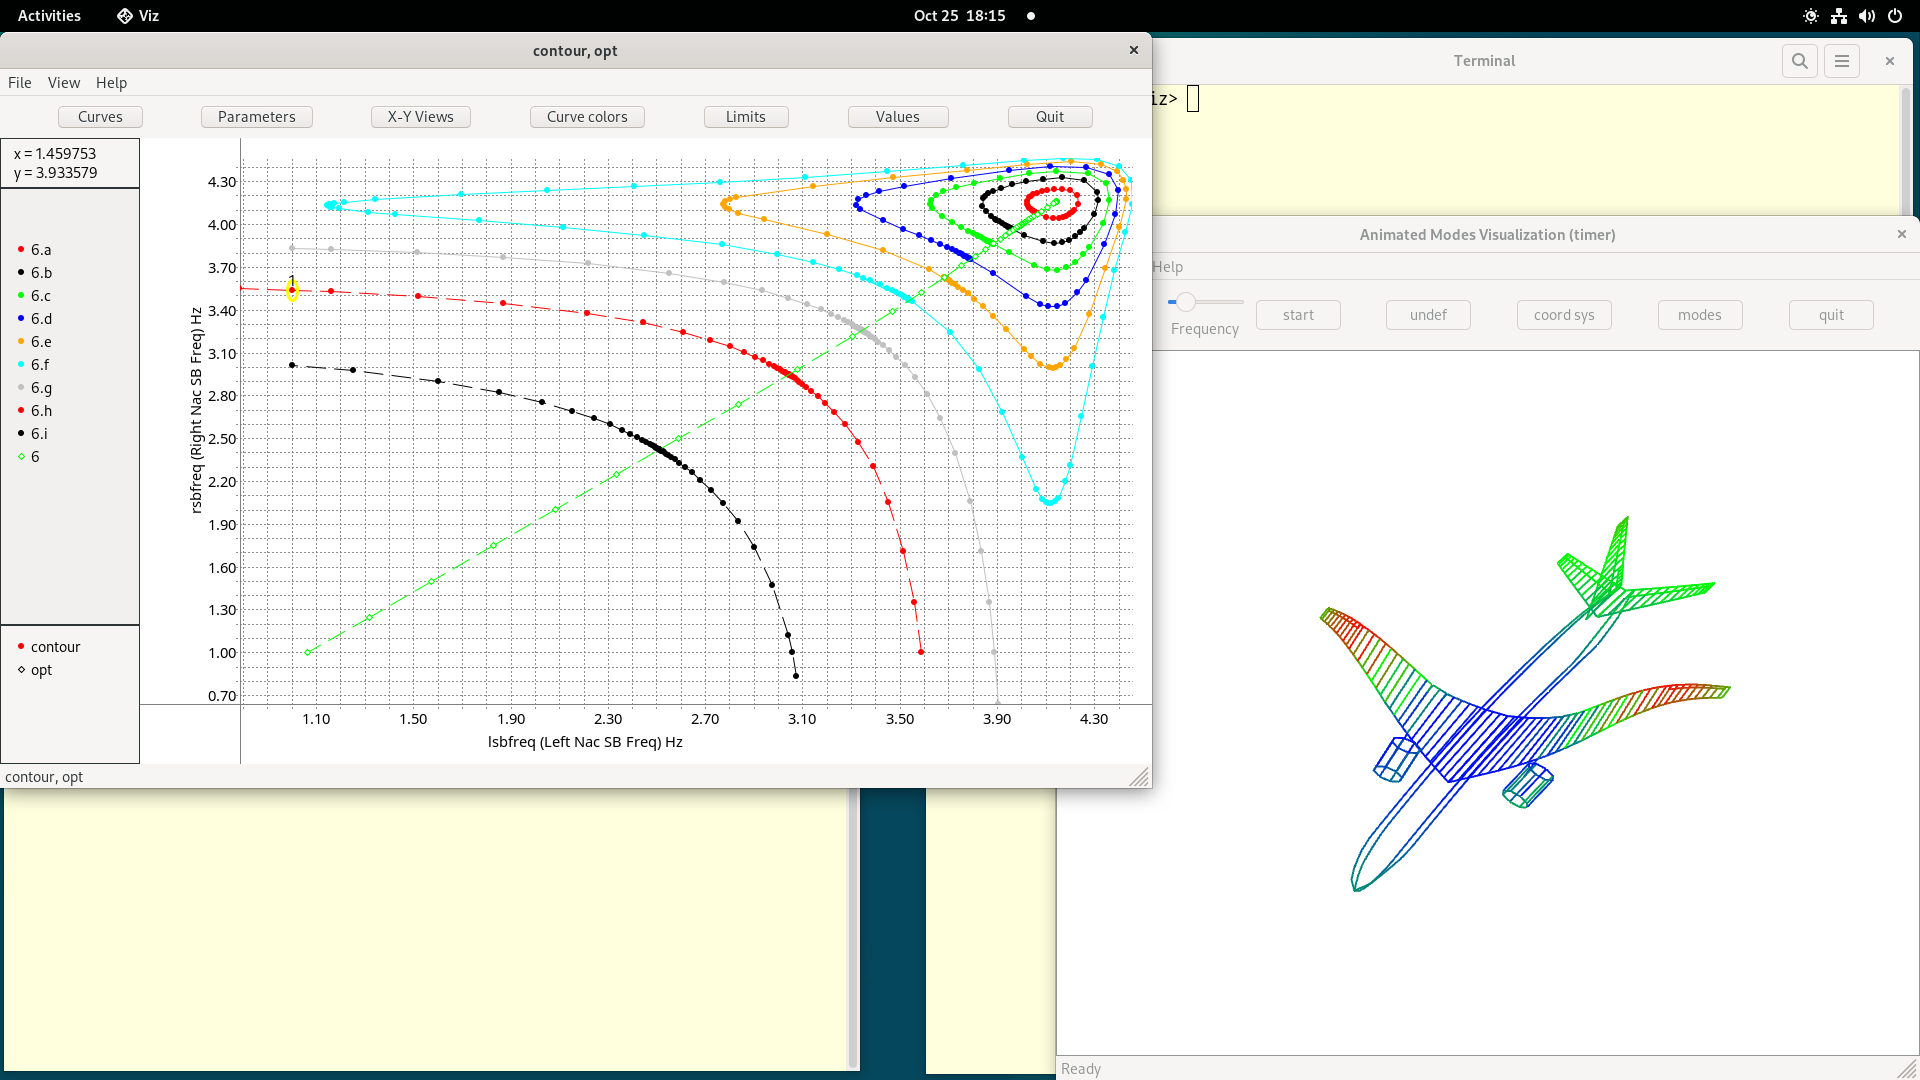
\includegraphics[height=9cm,width=16cm]{viz-amviz.png}
	\centering
\end{figure}
\vspace{2cm}

\Huge{Solving Flutter Equations}

\vspace{1cm}
\Large{Edward E. Meyer}

\vspace{1cm}
\Large{\ttfamily flapsconsulting@gmail.com}

\vspace{1cm}
\today

\vspace{3cm}
\small{Typeset by the author using the \LaTeX\ document processing system}
\end{center}

\author{Edward E. Meyer}

\chapter*{Preface}
\addcontentsline{toc}{chapter}{Preface}

This book grew out of a problem I faced when writing
my PhD thesis on flutter of windmill blades.
I needed to study the effects of varying properties such
as blade stiffness, mass properties, and aerodynamic properties,
but existing solution techniques made studies like these
very tedious.

A classmate suggested two techniques that seemed like a good
fit for my problem: continuation methods and automatic differentiation.
The key advantage continuation methods have over traditional
eigenvalue methods is the use of derivatives of the equations.
With these derivatives continuation methods can trace continuous curves,
in addition to solving flutter problems that are difficult or
impossible with traditional techniques.

When I joined Boeing after graduation I showed some results to
a senior flutter engineer who convinced me to let others
try the program I developed for my thesis.
It was an immediate success, largely due to its ability to
perform parameter studies.
During my 32 year career at Boeing I added numerous features,
but some of the more important ones had to wait until I retired.

In retirement I wrote a completely new implementation of the method in
modern C++, designed around nonlinear flutter, extensible plugins,
automatic differentiation, and parallel execution.
This program, called \emph{Fina}, serves as the computational foundation
for this book and is available as open-source software.
To generate the example problems, I added a small beam modeling capability,
which is ideal for demonstrating the solver's capabilities and providing
reproducible test cases for the journal articles I have written.

I have chosen to publish this book as open-access.
My ultimate goal is simply to share this knowledge and improve the
discipline of flutter analysis -- not to become fabulously wealthy.


\tableofcontents
\listoftables
\listoffigures

\mainmatter

% ------------------------------------------------------------------
% Introduction chapter
% ------------------------------------------------------------------
\chapter{Introduction}\label{chap:intro}

Flutter analysis, a critical discipline in aerospace engineering,
has historically relied on eigenvalue-based techniques for solving
its governing equations. This approach, while a natural evolution from
vibration analyses and well-suited for early aircraft designs with simpler
aerodynamics and limited degrees of freedom, has reached its limits in
the face of modern aerospace demands. Today's complex aircraft designs
often involve hundreds of degrees of freedom, intricate aerodynamic
interactions, and a burgeoning need to explore numerous configurations
to achieve optimal efficiency. The traditional eigenvalue framework
struggles to adequately capture these complexities and the multifaceted
influences on flutter behavior.

This book proposes and elaborates on a more robust and flexible approach
to flutter analysis: treating the flutter equations as a system of
nonlinear equations. This methodology not only offers a more accurate
representation of contemporary aerospace challenges but also fully
leverages the significant advancements in modern computer hardware
and software. By moving beyond the inherent constraints of eigenvalue
solvers, this nonlinear system approach empowers engineers to perform
more comprehensive and realistic flutter analyses.  This paradigm shift
enables the in-depth exploration of a wider range of design parameters and
environmental conditions, critical for developing the next generation of
high-performance and efficient aircraft.

\section{The Role of Flutter Analysis in Aircraft Design}
Throughout the design and certification of aircraft, rigorous flutter analyses
are essential to ensure a high degree of confidence in flight safety within
the defined \Newterm{flight envelope}. The flight envelope\index{flight envelope}
establishes the boundaries (e.g. velocity, altitude, payload) within which an
aircraft is certified safe to operate. Key tasks in this process include:
\begin{itemize}\label{sect:tasks}
	\item {\bf Neutral-stability search:}\index{neutral-stability}
			\index{stability!neutral} Identifying the boundary between decaying and growing
			oscillations, known as \Newterm{flutter speeds}. Due to its
			importance this is referred to as a \Newterm{core} analysis.
			\index{core flutter}\index{flutter!core analysis}
	\item {\bf Flight envelope coverage:} Repeating the flutter speed search across sufficient
	      points within the flight envelope to confirm the aircraft remains flutter-free.
	\item {\bf Parameter variations:} Investigating how flutter speeds change with various
	     design parameters (e.g. stiffness, control system) and flight-envelope
		  parameters (e.g. altitude, fuel loading, payload).
	\item {\bf Control system impact:} Evaluating the influence of control systems on
	      flutter characteristics.
	\item {\bf Nonlinear analysis:} Incorporating nonlinearities to make the analysis more
			realistic, changing the focus from flutter speeds
			to oscillations that either die out, increase until there is catastrophic
			damage to the structure, or are limited in amplitude due to the nonlinearities,
	     a phenomenon known as \Newterm{limit-cycle oscillation} or LCO.
		  \index{LCO|see {limit cycle oscillation}}\index{limit cycle oscillation|textbf}
		 	So analyses are further complicated by the need to account for amplitudes.
	\item {\bf Limit cycle stability determination:}
			determining what happens when the amplitude of an LCO is increased (or decreased);
			if the amplitude returns to the LCO amplitude the LCO is said to be \emph{stable},
			whereas if the amplitude continues to increase (decrease) it is said to be \emph{unstable}
			% assessing whether small perturbations in amplitude grow or decay to the limit cycle.
	     \index{limit cycle oscillation!stability}
\end{itemize}
Each of these tasks typically involves treating anywhere from one to hundreds
of aeroelastic modes.  As with any field involving extensive data analysis,
visualizing flutter data presents a significant challenge.

\section{A Numerical Continuation Approach}
Traditional flutter analysis methods formulate the problem as an eigenvalue
problem
\footnote{An excellent treatment of traditional methods is in \cite{demasi2024introduction}}.
While established, this approach presents several limitations:
\begin{itemize}
	\item {\bf Tedious Parameter Studies:} Parameter variations are cumbersome
		and time-consuming.
	\item {\bf Limited Scope:} Inability to directly incorporate control systems or
		nonlinearities.
	\item {\bf Inaccurate Mach Matching:} Solutions may not automatically compute with the
	    correct Mach number, requiring additional work if Mach fidelity is critical.
		extra work is required if that is important,
	\item {\bf Discontinuous Root Tracking:} While there have been attempts
		(\cite{desmarais1974automated}, \cite{eldred1995new}, \cite{chen2000damping})
		to automate the connection of the solutions comprising each mode,
		creating continuous curves is still largely a manual process
		\cite{demasi2024introduction}.
	\item {\bf Equation Manipulation:} Requires approximation and manipulation of the original
	   equations to fit the eigenvalue framework, obscuring their original form.
\end{itemize}
In contrast, treating the flutter equations as a system of nonlinear equations and
tracing the evolution of each mode in a continuous fashion with numerical
continuation avoids these drawbacks:
\begin{itemize}
	\item {\bf Unified Parameter Treatment:} All parameters---including
		generalized coordinates
	    and user-defined parameters---are treated equally. Consequently, every \Fina
		 analysis is inherently a parameter variation study.
	\item {\bf Broad Range of Formulations:} including nonlinearities,
		control systems, Laplace-domain aerodynamics, parametrized matrices,
		and gyroscopics.
	\item {\bf Accurate Mach Number:} Every solution point inherently possesses the
	     correct Mach number, provided the unsteady aerodynamic matrix is parametrized
		  with Mach in addition to reduced frequency.
	\item {\bf Continuous Solutions:} Solutions are computed using
	    numerical continuation, yielding continuous curves.
	\item {\bf Preserved Equations:} There is no need to manipulate the equations to
	     fit the continuation method, which simplifies the approach and makes it
		  significantly easier to explain and understand.
\end{itemize}

\section{How to Read This Book}
The basic idea behind using numerical continuation for solving flutter
equations is quite simple; as with most algorithms the programming details
are  what distinguish a computer program implementation from the basic
ideas. The first few chapters cover the basics of numerical continuation
and its application to flutter equations. Further chapters discuss
many of the details that went in to \Fina.

\begin{description}
	\item[\ref{chap:flutter-equations} Flutter Equations]
	Details the terminology, nomenclature, and equations used
	throughout this book.

	\item[\ref{chap:continuation} Numerical Continuation]
	Describes continuation methods in general and the particular type
	of continuation used in \Fina.

	\item[\ref{chap:AD} Automatic Differentiation]
	Describes a computer programming technique for computing exact derivatives
	automatically.

	\item[\ref{chap:application} Solving Flutter Equations]
	Details how numerical continuation can be used to solve flutter equations.

	\item[\ref{chap:nonlinear} Nonlinear Flutter]
	Shows how quasi-linear techniques like describing functions
	can be used to analyze nonlinear flutter.

	\item[\ref{chap:controls} Control Systems] Including control systems in
			the flutter equations.

	\item[\ref{chap:whirl} Whirl Flutter] Treating propeller-driven aircraft.

	\item[\ref{chap:tailoring} Customizing the Equations]
	Various methods are presented which allow customization of the
	flutter equations for particular applications: parameters, equations,
	and functions.

	\item[\ref{chap:substructuring} Substructuring for Flutter Analyses]
	Shows how substructuring techniques can be used in linear and nonlinear
	flutter analyses.

	\item[\ref{chap:examples} Example Problems] describes a few demonstration problems

	\item[\ref{chap:appendices} Appendices] gives various details
		regarding \Fina: obtaining, installing, using
                
\end{description}

% =================================================================
% Chapter Flutter Equations
% =================================================================
\newpage
\chapter{Flutter Equations}\label{chap:flutter-equations}
Over the years there have been a variety of formulations of the
linear flutter equation in the frequency domain (\Sectref{sect:formulations}.
The intent here is to present a very general formulation, making few
assumptions.

Flutter equations comprise a set of matrices, several parameters, compatible
\emph{generalized coordinates} (\Gc), and a transformation matrix
$\Phi$ that converts the generalized coordinates to physical
displacements:
\begin{displaymath}
\Vector{\chi} = \Matrix{\Phi}\Vector{q}
\end{displaymath}

Flutter equations can be characterized as \emph{nonlinear} or
\emph{linear} according to whether the matrices
are or are not dependent on displacement amplitudes.
In addition to the traditional mass, stiffness, and aerodynamic
matrices a few are included here that are awkward or impossible to include
in traditional methods.

\section{Nomenclature}\label{sect:flut-nomenclature}
\index{nomenclature!flutter equation}
A hat on a variable means that it is complex and has an
equivalent real representation of the variable without the hat
(\Sectref{sect:real-conversion}).  For example $\hat{\Vector{y}}$ and
$\Vector{y}$ are the complex and real representations of the eigenvector.
\begin{small}
\noindent\begin{longtable}{@{}lcl@{}}
$a$ & & sonic velocity \\
$c$ & & reference length for reduced frequency (default 2)
	\index{=c@$c$ (ref. length)} \\
$\mathbb{C}^n$, $\mathbb{C}^{m \times n}$ & & the complex $n$-vectors
   and $m$ by $n$ matrices \\
$\hat{\Matrix{D}}$, $\Matrix{D}$ & & complex ($n_e,n_e$) dynamic matrix
	and it's real equivalent (\Eqn{eqn:flut} \\
$\Matrix{M}$, $\Matrix{K}$, $\Matrix{G}$,
	&  & $(n_e,n_e)$ mass, stiffness, gyroscopic, viscous damping, \\
$\Matrix{C}$, $\Matrix{Q}$, $\Matrix{T}$ & & unsteady aero and
   user-defined matrices (\Eqn{eqn:flut}) \\
$M$ & & Mach number $V/a$ \\
$n_e$ & & the number of complex \Gc \\
$q$ & & dynamic pressure $\rho V^2/2$ \\
$\Vector{q}$ & & vector of $n_e$ complex \Gc\ 
	$\eta\Vector{\hat{y}}$ (\Eqn{eqn:gcsplit}) \\
$\Vector{\chi}$ & & real vector of physical motion of the structure
	at discrete points (\Eqn{eqn:motion}) \\
$s$ & & Laplace variable $\sigma + i\omega$ \\
$\bar{s}$ & & $sc/2V$, complex reduced frequency \\
$V$ & & velocity (true airspeed) \\
$\Vector{\hat{y}}$, $\Vector{y}$ & & complex eigenvector and its real
	equivalent (\Eqn{eqn:flut}) \\
$\eta$ & & 2-norm of the \Gc\ (\Eqn{eqn:normalization}) \\
$\omega$ & & oscillation frequency (imaginary part of the complex frequency) \\
$\bar{\omega}$ & & reduced frequency $\omega c/2V$ \\
$\Matrix{\Phi}$ & & transformation from generalized to physical coordinates (\Eqn{eqn:motion}) \\
$\rho$ & & fluid density \\
$\sigma$ & & stability factor (real part of the Laplace variable) \\
$\bar{\sigma}$ & & reduced stability factor $\sigma c/2V$ \\
$\|\Vector{y}\|_2$ & & 2-norm of vector $\Vector{y} =
   \sqrt{\Vector{y}^*\Vector{y}}$ \index{2-norm!complex}\\
$(\;)^T$ & & transpose \\
$(\;)^*$ & & conjugate transpose \\
\end{longtable}
\end{small}

\section{Matrices}
\subsection{Mass and Stiffness}
The starting point for most flutter analyses is a set of mass,
stiffness, and unsteady aerodynamics matrices, created by
a large finite-element program such as Nastran, a tiny beam-modeling
program such as in \Fina, or something in-between.
They are usually predicated on two equivalent assumptions:
\begin{itemize}
	\item they are valid only for infinitesimal displacements,
	\item they are not functions of displacements
\end{itemize}
in other words, they do not take into account the fact that deflections
of the structure can affect changes in stiffness and aerodynamics,
and flutter equations using them are called \emph{linear flutter equations}.

\subsection{Unsteady Aerodynamics}
Likewise, unsteady aerodynamic matrices, created for instance
with one of the many implementations of the doublet lattice method
\cite{demasi2024introduction}, make the small displacement assumption,
and are also called linear. Unsteady aerodynamics are also dependent
on the Mach number ($M$).
The widely-used doublet lattice method
is formulated in the frequency domain, resulting in matrices that
are functions of the so-called \emph{reduced frequency}
$\bar{\omega} = \frac{\omega c}{2V}$, and can be formulated to include
the reduced stability factor $\bar{\sigma} = \frac{\sigma c}{2V}$
\cite{cunningham1984generalization}.
In its most general form then the unsteady aerodynamic matrix is
a function of four parameters: $\omega$, $\sigma$, $M$, and $V$.

In practice, aerodynamic matrices are usually computed at several values
of reduced frequency, one or more values of Mach, and possibly
multiple values of reduced stability factor, then fitted with
1, 2, or 3 dimensional interpolation functions.
Unless there is interest in behavior of modes away from flutter
it is usually not necessary to interpolate with respect to reduced
stability factor since it will not change the flutter speed;
more important is the Mach number, which \emph{will} affect the flutter speed.

\subsection{Additional Matrices}
Other, less common matrices include:

\begin{description}
	\item[\bf gyroscopics] a structure may contain one or more spinning
	parts such as propellers represented in matrix $\Matrix{G}$
	\index{gyroscopics}; \Chapref{chap:whirl} has more details.

	\item[\bf viscous damping] $\Matrix{C}$, sometimes represented as
		proportional to the mass and stiffness matrices:
			\mbox{$\Matrix{C} = \alpha\Matrix{K} + \beta\Matrix{M}$}.
		like gyroscopics, viscous damping is dependent on $s$.
		\index{damping!viscous}

	\item[\bf control systems] are contained in a matrix $\Matrix{T}$,
		which in \Fina can be created as a custom function written by the user,
		or a linear, time invariant (LTI) control system designed, for
		example, in \Simulink. Chapter \ref{chap:controls} has more details.
\end{description}

\section{Parameters}
Flutter equations are traditionally presented in terms of just a few
parameters: $\sigma, \omega$, and $q$, with reduced frequency ($\bar\omega$)
and Mach number ($M$) often included. These and other parameters are
listed in \Tableref{table:params-eqns} together with some possible equations.


\begin{table}[ht]	% table:params-eqns
\centering
% \begin{scriptsize}
% \begin{footnotesize}
% \begin{small}
\begin{tabular}{|c|l|l|} \hline
Symbol			& \CCol{Description}					& \CCol{Equations}			\\ \hline \hline
$a$            & sonic velocity						& $a(z)$\dag							\\ \hline
$b$            & $\bar{\omega}$ reference length& \ddag									\\ \hline
$d$            & structural damping					& \ddag									\\ \hline
$\delta$			& pressure ratio						& $P(z)/P(0)$							\\ \hline
$\eta$         & amplitude of oscillation			&  \ddag									\\ \hline
$g$            & growth factor						& $2\sigma/\omega$          		\\ \hline
$M$            & Mach number							& $V/a $									\\ \hline
$\omega$       & frequency								& $\bar{\omega} V/b$				\\ \hline
$\bar{\omega}$ & reduced frequency					& $\omega b/V$						\\ \hline
$P$            & static pressure 					& $P(z)$\dag							\\ \hline
$P_t$          & total pressure 						& $P + q$								\\ \hline
$q$            & dynamic pressure					& $\rho V^2/2 = \rho(0) V_e^2/2$	\\ \hline
$q_c$          & calibrated dynamic pressure		& $P(1 + 0.2M^2)^{3.5} - 1$		\\ \hline
$\rho$         & fluid density						& $\rho(z)$\dag						\\ \hline
$\bar{\sigma}$ & reduced stability factor			&  $\sigma b/V$						\\ \hline
$\sigma$       & stability factor					& \ddag									\\ \hline
$V_c$          & calibrated airspeed				& $V_e[1+\frac{1}{8}(1-\delta)M^2+
										\frac{3}{640}(1-10\delta^2+9\delta^2)M^4]$			\\ \hline
$V_e$          & equivalent airspeed 				& $V \sqrt{ \rho(z)/\rho(0)}
																	= \sqrt{2q/\rho(0)}$				\\ \hline
$V$            & true airspeed 						& $Ma(z) = \omega b/\bar{\omega}
										= \sqrt{2q/\rho(z)} = V_e\sqrt{\rho(0)/\rho(z)}$	\\ \hline
$z$            & altitude 								& $z(\rho)$\dag						\\ \hline
\multicolumn{3}{|l|}{\dag \hspace{2mm}table lookup in std atmosphere tables}		\\
\multicolumn{3}{|l|}{\ddag \hspace{2mm}always either constant or independent}		\\ \hline
\end{tabular}
% \end{scriptsize}
% \end{footnotesize}
% \end{small}
\caption{Parameter equations} \label{table:params-eqns}
% index all symbols. Prefix them with an equals sign
% to force them to appear first.
\index{parameters!builtin}
\index{builtin!parameters}
\index{=a@$a$ (sonic velocity)}\index{sonic velocity}
\index{=b@$b$ (reference length)}\index{reference length}
\index{=d@$d$ (structural damping)}\index{structural damping}
\index{=eta@$\eta$ (\Gc\ norm)}\index{generalized coordinates!norm}
\index{=g@$g$ (growth factor)}\index{growth factor}
\index{=m@$M$ (Mach number)}\index{Mach number}
\index{=omega@$\bar{\omega}$ (reduced frequency)}\index{reduced frequency}
\index{=omega@$\omega$ (frequency)}\index{frequency}
\index{=ps@$P$ (static pressure)}\index{static pressure}\index{pressure!static}
\index{=p0@$P_{0}$ (ref. static pressure)}\index{reference static pressure}
\index{=qc@$q_c$ (calibrated dynamic pressure)}\index{calibrated dynamic pressure}\index{pressure!calibrated dynamic}
\index{=q@$q$ (dynamic pressure)}\index{dynamic pressure}\index{pressure!dynamic}
\index{=rho@$\rho $ (density)}\index{fluid density}\index{density}
\index{=rho0@$\rho_{0}$ (ref. density)}\index{reference density}\index{density!reference}
\index{=sigma@$\Rsf$ reduced stability factor}
\index{=sigma@$\sigma$ stability factor}
\index{=vc@$V_{c}$ (calib. airspeed)}\index{calibrated airspeed}\index{airspeed!calibrated}
\index{=ve@$V_{e}$ (equiv. airspeed)}\index{equivalent airspeed}\index{airspeed!equivalent}
\index{=vt@$V_{t}$ (true airspeed)}\index{true airspeed}\index{airspeed!true}
\index{=z@$z$ (altitude)}\index{altitude}
\end{table}



\section{Linear Flutter Equations}\label{sect:complexflutter}
Flutter equations in the frequency domain are based on
the assumption that the physical motion of the structure at discrete points
($\Vector{\chi}$) as a function of time
is related to a set of complex \Gc\
$\Vector{q}$ by complex exponentials
\begin{equation}
\Vector{\chi}(t) = \Re(\Vector{q}e^{st})
\end{equation}
or more commonly, by modal-reduction\index{modal reduction} \Gc:
\begin{align} \label{eqn:motion}
\Vector{\chi}(t) & =  \Re \left(\Matrix{\Phi}\Vector{q}e^{st}\right) \nonumber \\
              & =  \Re \left[\Matrix{\Phi}\Vector{q} e^{\sigma t}
				  			\left(\cos \omega t + i \sin \omega t \right) \right]
\end{align}
where $\Matrix{\Phi}$ \index{=Phi@$\Matrix{\Phi}$!modal reduction} is typically
a matrix of vibration modes and component modes (\Chapref{chap:substructuring}),
$t$ is time, $s = \sigma + i\omega$ is the complex frequency, $\omega$
is the frequency and oscillations are growing, neutral or decaying if the
\Newterm{stability factor} $\sigma$ is positive, zero or negative, respectively.\index{factor!stability}

It proves useful, especially when treating nonlinear flutter
(\Sectref{sect:separation})\index{GC!splitting}, to split the generalized
coordinate vector into an eigenvector $\hat{\Vector{y}}$
and a real scalar ($\eta$):
\begin{equation}\label{eqn:gcsplit}
	\Vector{q} = \eta \hat{\Vector{y}}
\end{equation}
and to require $\hat{\Vector{y}}$ always have unit magnitude in the 2-norm:
\begin{equation}\label{eqn:normalization}
	\|\hat{\Vector{y}}\|_2^2 = \hat{\Vector{y}}^*\hat{\Vector{y}} = \Vector{y}^T\Vector{y} = 1
\end{equation}
with one component constrained to be real to make the normalization unique:
\begin{equation}\label{eqn:phase}
 	\Im(\hat{y}_k) = 0
\end{equation}
Then $\eta$ determines the magnitude of oscillation and is the 2-norm
of the generalized coordinate vector.

Most traditional flutter solution techniques allow for only mass, stiffness,
and unsteady aerodynamic matrices. By treating the equations as a system
of nonlinear equations instead of an eigenvalue problem, that restriction
is removed and a much more general formulation is possible.
Including all the matrices discussed above the flutter equations can
be written as
\begin{equation}\label{eqn:flut}
	% \Vector{\hat{f}}_y &= \Vector{D\hat{y}} = \Vector{0}\;\;\in \mathbb{C}^{n_e} \nonumber \\
	\left[ s^2 \Matrix{M} + s \Matrix{G} + s \Matrix{C} +
		 \Matrix{K} - q \Matrix{Q} (\bar{s},M)
		 + \Matrix{T} \right] \hat{\Vector{y}} =
		 	\hat{\Matrix{D}}\hat{\Vector{y}} = \Vector{0}
\end{equation}

This is a system of $n_e$\index{ne@$n_e$} complex equations, homogeneous
in $\Vector{\hat{y}}$, and nonlinear in one or more parameters. In spite of
this, it is termed a \emph{linear} flutter equation if none of the matrices are
dependent on $\Vector{q}$.

In addition to allowing for more matrix types than usual, solving as nonlinear
equations allows the matrices to be nonlinear functions of user-defined parameters
and the standard parameter in \Tableref{table:params-eqns}.
This ability is very important for carrying out the many parameter studies
necessary for designing and certifying aircraft.
For example, the mass matrix might be a function of a user-defined fuel parameter;
the stiffness matrix might have structural damping applied to some elements;
and the gyroscopic matrix might be a function of one or more spin rates.

\section{Various Formulations}\label{sect:formulations}
Many different formulations
\footnote{although these are typically called ``methods'' they are really
	just different ways of formulating the equations to solve as an
	eigenvalue problem; numerical continuation could also be used to solve them.}
of flutter equations have been proposed
over the past 50 years, usually with the goal of increasing the accuracy
and/or decreasing the cost of solutions. A partial list includes
(\cite{demasi2024introduction} presents these in detail):
\begin{description}
	\item[V-g method] (also known as the k-method or American method)
		\cite{hassig1971approximate} the decaying (growing)
		of oscillations is approximated by adding positive (negative) structural
		damping, 
	\item[p-k method] (sometimes called the British method) solves for
		the Laplace variable $s = \sigma + i\omega$ as an eigenvalue problem
		\cite{hassig1971approximate}, iterating to get the correct reduced frequency,
	\item[non-iterative p-k method]\cite{pitt1999new} uses interpolation instead of
		iteration to get the correct reduced frequency,
	\item[g-method]  uses the derivative of unsteady aerodynamics with respect to
			reduced frequency and the Cauchy-Riemann equations to extend the
			aerodynamic matrix into the Laplace domain for small values of the real
			part of the complex reduced frequency $\bar{\sigma}$\cite{chen2000damping},
	\item[Generalized Aeroelastic Analysis method] uses modifications to the
			doublet-lattice method to create unsteady aerodynamics that are functions
			of complex reduced frequency ($\bar{s}$), i.e. Laplace-domain aerodynamics
			\cite{edwards2008flutter},
	\item[p-method] uses unsteady aerodynamics in the Laplace domain
			to improve the accuracy at non-zero values of $\sigma$.
			\cite{haddadpour2009true}
	\item[Complex Velocity] Using complex velocity squared as the eigenvalue,
		setting $\sigma=0$, and solving an eigenvalue problem at several
		reduced frequencies, a reduced frequency where the eigenvalue is
		real is a flutter point \cite{pitt2000complex}.
\end{description}
A significant limitation of traditional flutter solution methods stems
from their formulation as an eigenvalue problem. This approach inherently
restricts their application, precluding the direct incorporation of
control equations or nonlinearities. Furthermore, conducting comprehensive
parameter studies becomes a tedious endeavor. While some modifications
to the formulation may allow for the inclusion of gyroscopic terms,
this is not a universally straightforward capability.

While these formulations aim to improve solution accuracy under
non-flutter conditions, they yield identical flutter speeds, provided the
aerodynamics are at the same Mach number. However, this often overlooks
the critical fact that the chosen Mach number is usually incorrect for
the actual flutter condition.

In stark contrast, approaching the flutter equations as a system
of nonlinear equations overcomes these limitations entirely. The
flutter equation employed here offers far greater flexibility,
accommodating control systems, gyroscopic effects, viscous damping,
and nonlinearities. Crucially, it can incorporate unsteady aerodynamics
that are functions of both complex reduced frequency and Mach number,
eliminating the need for iterative Mach matching. Additionally, any
of the matrices within this framework can be quasi-linear functions of
discrete generalized coordinates.

Example problem \Code{methods.fp} \Sectref{ex:formulation-comp}
compares these methods using \Fina,
demonstrating the versatility of the approach. An interesting finding from
this example is the importance of using correct Mach numbers at each solution
point which is possible in \Fina by interpolating with respect to Mach in
addition to reduced frequency.\index{Mach number!matched}

% =================================================================
% Chapter Numerical Continuation
% =================================================================
\newpage
\chapter{Numerical Continuation}\label{chap:continuation}

\section{Nomenclature}\label{sect:pac-nomenclature}
\begin{small}
\index{numerical continuation!nomenclature}
\noindent\begin{longtable}{@{}lcl@{}}
$\Vector{f}$ & & vector of $n$ real, nonlinear equations \\
$\Vector{h}^i$ & & $i\text{th}$ corrector step (\Eqn{eqn:h}) \\
$\Matrix{J}$ & & Jacobian matrix of partial derivatives (\Eqn{eqn:jacobian}) \\
$\Matrix{Q}$, $\Matrix{R}$ & & QR factors of the transposed Jacobian (\Eqn{eqn:qr}) \\
$\mathbb{R}^n$, $\mathbb{R}^{m \times n}$ & & the real $n$-vectors and $m$ by $n$ matrices \\
$\Vector{t}$ & & tangent vector (\Eqn{eqn:Jt}) \\
$\|\Vector{x}\|_2$ & & 2-norm of vector $\Vector{x} =
   \sqrt{\Vector{x}^T\Vector{x}}$ \index{2-norm!real}\\
$\|\Vector{x}\|_\infty$ & & maximum-norm of vector $\Vector{x} = {\displaystyle \max_{i=1,\ldots n} |x_i|}$ \\
$\Vector{w}$ & & projection vector (\Eqn{eqn:project}) \\
$\Vector{x}$ & & independent variables \\
$\Vector{x}_j^i$ & & $i\text{th}$ corrector iteration at the $j\text{th}$
   continuation step (\Eqn{eqn:predictor}) \\
$x_i$ & & $i\text{th}$ element of vector $\Vector{x}$ \\
$\tau$ & & arclength along a curve (\Figref{fig:pac}) \\
$\Step$ & & stepsize in the continuation process (\Eqn{eqn:predictor}) \\
$()^T$ & & transpose \\
\end{longtable}
\end{small}
\index{numerical continuation!nomenclature}
\index{continuation|see {numerical continuation}}

\section{Background}\label{sect:background}
Continuation methods have been developed by mathematicians since the
mid-20th century as a means for solving nonlinear equations,
and simultaneously by engineers where they are known as \emph{incremental methods}
\cite{oden2006finite}.
The recognition that incremental methods belong to the class of methods
known as continuation methods put them on a more solid theoretical footing
\cite{rheinboldt1981numerical}.

Modern numerical continuation is a class of techniques for solving
underdetermined systems of nonlinear equations:
\begin{align}\label{eqn:fx}
\Vector{f}(\Vector{x}) = \Vector{0} & \in \mathbb{R}^{m} \nonumber \\
\Vector{x} & \in \mathbb{R}^{n}
\end{align}
where the number of equations $m$
is fewer than the number of independent variables $n$.
Because there are fewer equations than unknowns, there are an infinite
number of solutions.
Depending on the difference $n-m$, the solution space consists of
curves ($n-m = 1$), surfaces ($n-m = 2$), volumes ($n-m = 3$), and so on
\footnote{throughout this book, only curves are considered; with the
exception of \Sectref{sect:optim}, $n = m+1$}.

Most continuation methods use a predictor-corrector approach,
reminiscent of ordinary differential equation solvers.
For the predictor, many methods
(\cite{cardani1978continuation}, \cite{yu2020nonlinear},
\cite{rheinboldt1983algorithm},
\cite{allgower1990numerical} p. 3),
choose a particular parameter to increment throughout the tracing of curves,
but these methods can fail if the curve has \Newterm{limit points} in
this continuation parameter.
A limit point is where a curve reaches a minimum or maximum in the continuation
parameter, and the tangent to the curve has a zero component for that parameter,
so that incrementing that parameter does not increment the distance along the
curve. Locally parametrized continuation methods \cite{rheinboldt1983locally}
avoid this problem\index{numerical continuation!locally parametrized}
by choosing the best parameter (in some sense) to increment at each point.

For the corrector phase these methods either constrain the continuation parameter
to remain constant, or add a constraint to force corrections to be perpendicular to
the tangent. Either approach allows corrections to be computed by solving a
square system of equations using efficient linear equation solvers.

\section{Pseudo-Arclength Continuation}\label{sect:pseudo}
\index{numerical continuation!pseudo-arclength}
In contrast to most continuation methods, here all of the independent
variables ($\Vector{x}$) are treated equally -- there is no
``continuation parameter'', simplifying both the presentation and
programming of the method.

As with all continuation methods, tracing a curve starts from a known solution
$\Vector{x}_0$, computing points on the curve $\Vector{x}_1$, $\Vector{x}_2$, 
$\Vector{x}_3$,  ...  $\Vector{x}_n$.
At a converged solution $\Vector{x}_j$, the process for computing the
next point is shown in \Figref{fig:pac}.
\begin{figure}[ht] 	% complains if h
		\includegraphics[height=8cm,width=10cm]{pac.eps}
	\centering
	\caption{Continuation from $\Vector{x}_j$ to $\Vector{x}_{j+1}$}\label{fig:pac}
\end{figure}
where $\tau$ is a measure of distance along the curve (the \emph{arclength}),
$\Delta \tau$ is a
small  increment in $\tau$, which when multiplied by the tangent to
the curve at $\Vector{x}_j$ gives a prediction (
$\Vector{x}_{j+1}^0$) of the next solution. The fact that the stepsize
$\Delta\tau$ is an approximation to the arclength between
$\Vector{x}_j$ and $\Vector{x}_{j+1}$ gives rise to the name
\emph{pseudo-arclength continuation}.

Mathematically the next point is found by a 2-step process:
\begin{itemize}
	\item a solution is \emph{predicted} by multiplying the tangent to the curve
		by a small number, the stepsize $\Step$:
		\begin{equation}\label{eqn:predictor}
			\Vector{x}_{j+1}^0 = \Vector{x}_j + \Step \Vector{t} \nonumber
		\end{equation}
	\item the predicted solution is \emph{corrected} with a Newton-type iteration:
		\begin{align}
			\label{eqn:corrector}
			\Matrix{J}(\Vector{x}^{i})\Vector{h}^i &=
				-\Vector{f}(\Vector{x}^{i}) \nonumber \\
			\Vector{x}^{i+1} &= \Vector{x}^{i} + \Vector{h}^i \hspace{1cm}
				i=0, 1, 2, ...\;\text{convergence}
		\end{align}
		where $\Matrix{J}$ is the Jacobian, a matrix of derivatives
		of $\Vector{f}$ with respect to $\Vector{x}$.
\end{itemize}

\subsection{The Jacobian}
The most important term in the method is the \emph{Jacobian} matrix
$\Matrix{J}$, an $(m,n)$ matrix of derivatives of $\Vector{f}$ with
respect to $\Vector{x}$:
\begin{equation}\label{eqn:jacobian}
	\Matrix{J} = \Vector{f}'(\Vector{x}) =
		\frac{\partial \Vector{f}}{\partial \Vector{x}} =
		\left[\frac{\partial f_i}{\partial x_j}\right]
\end{equation}
The Jacobian is important because errors in computing it can make the
continuation process fail or take excessive computer time;
it is also used to predict the next solution in the tracking process.
The burden of computing these derivatives is made much easier by the use of
\emph{automatic differentiation}\index{automatic differentiation!in numerical continuation},
as detailed in \Chapref{chap:AD}.

\subsection{The Tangent}\label{sect:the-tangent}
Considering $\Vector{x}$ to be a function of the arclength ($\tau$) along the
curve, the tangent vector to the curve is the derivative of $\Vector{x}$
with respect to this distance: $\Vector{t} = d\Vector{x}/d\tau$.
Moreover, the tangent has unit length, since
	$d\tau^2 = d\Vector{x}^T d\Vector{x} = \|d\Vector{x}\|_2^2$,
\begin{displaymath}
\Vector{t}^T\Vector{t} =
	\left(\frac{d\Vector{x}}{d\tau}\right)^T \frac{d\Vector{x}}{d\tau}
	= \frac{d\Vector{x}^T d\Vector{x}}{d\tau^2} = 1
\end{displaymath}

Computing the tangent relies on the fact that the tangent is the null
vector of the Jacobian\footnote{although the focus here is on Jacobians with a single
null vector, multiple null vectors will be treated in \Sectref{sect:optim}.},
seen by differentiating \Eqn{eqn:fx} with respect to $\tau$:
\begin{equation}\label{eqn:Jt}
	\frac{d\Vector{f}}{d\tau} = \frac{\partial\Vector{f}}{\partial\Vector{x}}\frac{d\Vector{x}}{d\tau}
		= \Vector{Jt} = \Vector{0}
\end{equation}
There are many ways to compute the null vector; two are particularly efficient here:

\subparagraph{1)} Computing by solving a system of linear equations:
\begin{itemize}
	\item choose one component of the tangent to implicitly set to 1, 
		for convenience the last component,
	\item extract the last column of the Jacobian, call it $\Vector{b}$,
	\item extract the remaining columns into a matrix $\Matrix{A}$
	\item solve the linear system $\Matrix{A}\Vector{z} = \Vector{b}$ for
		$\Vector{z}$,
	\item then $\Vector{q}_2 =
		\left\{ \begin{array}{c}
			\Vector{z} \\
			-1
		\end{array} \right\}$ is the null vector.
\end{itemize}

\subparagraph{2)} If the corrector process uses a QR factorization
of the transposed Jacobian as this procedure does, the null  
vector is the vector $\Vector{Q}_2$ of the last factorization in the
corrector process.

The null vector must be normalized to 1 and the sign adjusted so that
$\Vector{t}_{j-1}^T \Vector{t}_j > 0$, that is, so that it points in roughly the
same direction as the previous step.

\subsection{The Predictor}
The stepsize $\Step$ must be chosen carefully. Too large a step,
and the corrector may not converge or may converge to the wrong root;
too small a step means extra work. Den Heijer and Rheinboldt
\cite{denheijer1981steplength} studied the problem of computing
step sizes, and Rheinboldt \cite{rheinboldt1983locally}
produced a continuation code using their algorithm, taking in to account
the curvature and the rate and quality of corrector convergence.
No attempt will be made to present the technique; a good summary is given
in \cite{rheinboldt1986numerical}, with FORTRAN source code in \cite{pcon61},
and translated into \Cpp in \Fina.
\index{numerical continuation!stepsize}

\subsection{The Corrector}
Because the Jacobian has more columns than rows the system of
linear equations in the corrector step \Eqn{eqn:corrector} is
an \emph{underdetermined} set of linear equations with an infinity
of solutions. The smallest solution is the one closest to the
predicted point; known as the \emph{minimum norm}
solution (\cite{golub2013matrix} \S 5.6.2), it can be computed with a
QR factorization of the transpose of $\Vector{J}$:
\begin{equation}
\label{eqn:qr}
\Matrix{J}^{t} = \Matrix{QR} = \left[ \Matrix{Q}_1 \;\; \Matrix{Q}_2 \right]
	\left[ \begin{array}{c}
		\Matrix{R}_1 \\
		\Matrix{0} \\
	\end{array}\right] = \Matrix{Q}_1 \Matrix{R}_1
\end{equation}
where $\Matrix{Q}$ is an $(n,n)$ orthogonal matrix, and $\Matrix{R}_1$
is an $(m,m)$ upper-triangular matrix. Because we are only considering
curves, $n = m+1$, $\Vector{Q}_2$ is a vector.

Substituting \Eqn{eqn:qr} into \Eqn{eqn:corrector} yields the
minimum-norm solution $\Vector{h}^i$:
\begin{equation}
\label{eqn:h}
\Vector{h}^i = - \Matrix{Q}_{1} \Matrix{R}_{1}^{-t} \Vector{f}(\Vector{x}^i)
\end{equation}
and substituting this into \Eqn{eqn:corrector} gives a closer approximation
to the solution.

Figure \Figref{fig:pacmn} compares the 2 traditional correction methods
with the minimum-norm method used here. In general the minimum-norm method
yields the closest correction, and should result in slightly fewer iterations.

Because computing the Jacobian and factorizing it is one
of the more expensive processes in any continuation method,
a cost-saving technique is to evaluate and factorize the Jacobian
at the beginning of the corrector step, then iterate using these factors
in \Eqn{eqn:h}. If convergence is not achieved within a few iterations,
re-evaluate the Jacobian and repeat the QR factorization.
\begin{figure}[ht] 	% complains if h
		\includegraphics[height=8cm,width=10cm]{pacmn.eps}
	\centering
	\caption{3 methods for the corrector process }\label{fig:pacmn}
\end{figure}

\subsection{Convergence}
\Eqn{eqn:corrector} with \Eqn{eqn:h} is repeated until some convergence criteria
are met. Following \cite{rheinboldt1981numerical}, convergence criteria are
divided into strong and weak acceptance criteria, using tolerances
\begin{description}
	\item[$\epsilon_m$,] machine epsilon: the largest number such that $1.0+\epsilon_m = 1.0$
	\item[$\epsilon_a$,] absolute tolerance: $\sqrt{\epsilon_m}$
	\item[$\epsilon_r$,] relative tolerance: $\sqrt{\epsilon_m}$
	\item[$\epsilon_h$,] correction tolerance: $\epsilon_a + \epsilon_r \|\Vector{x}^j\|_\infty$
	\item[$j_{\text{max}}$] maximum number of corrector iterations
\end{description}
\subsubsection{Strong acceptance:}
		$\|\Vector{f}^j\|_\infty < \epsilon_a$ and
		$\|\Vector{h}^j\|_\infty < \epsilon_r$
\subsubsection{Weak acceptance:}
	\begin{gather}
			\|\Vector{f}^j\|_\infty < 8\epsilon_m \nonumber \\
		\text{or}\;\; \|\Vector{f}^j\|_\infty +
				\|\Vector{f}^{j-1}\|_\infty < \epsilon_a
				\;\;\text{and}\;\; \|\Vector{h}^j\|_\infty < 8\epsilon_h
					\;\;\text{for some}\;\; j \ge 1 \nonumber \\
		\;\;\text{or}\;\; \|\Vector{f}^j\|_\infty \le 8\epsilon_a \;\;\text{and}\;\;
				 \|\Vector{h}^j\|_\infty + \|\Vector{h}^{j-1}\|_\infty
					\le \epsilon_h \;\;\text{for some}\;\; j \ge 2 \nonumber
	\end{gather}

On the other hand, nonconvergence is declared if one of the following
conditions are met:
\subsubsection{Nonconvergence:}
	\begin{gather}
		j \ge j_{\text{max}} \nonumber \\
		\|\Vector{f}_j\|_\infty \ge \|\Vector{f}_{j-1}\|_\infty \;\;\text{for some}\;\;j \ge 1 \nonumber \\
		\|\Vector{h}_j\|_\infty \ge \theta\|\Vector{h}_{j-1}\|_\infty \;\;\text{for some}\;\;j \ge 2 \nonumber
	\end{gather}

\section{Issues}\label{sect:issues}\index{numerical continuation!issues}
Several things can go wrong in a continuation procedure, including
\begin{itemize}
	\item nonconvergence of the corrector: retry the step with a smaller stepsize.
		If this does not cure the problem the Jacobian should be checked by finite
		differencing.
	\item large angle between consecutive tangents. This may indicate
		a discontinuity in the curve, mode switching, a bifurcation,
		or just a sharp change in the curve; retry the step with a smaller
		stepsize, monitoring the angle and the distance along the curve.
		When the distance exceeds the original stepsize there are 3 possibilities:
		\begin{enumerate}
			\item reducing the stepsize reduced the angle substantially so there
				is not a discontinuity or mode switching,
			\item the angle has not reduced substantially so there appears to
				be a discontinuity between two of the steps taken while monitoring,
			\item there is a bifurcation between two of the steps; the procedure
				outlined in \Sectref{sect:bifurcation} shows how to branch from
				the bifurcation point.
		\end{enumerate}
	\item a singular Jacobian indicates a bifurcation; very rare and
		a bifurcation is more likely to be discovered using the
		technique in \Sectref{sect:bifurcation}.
\end{itemize}

\section{Homotopy}\label{sect:homotopy}
\index{numerical continuation!homotopy}\index{homotopy}
One of the earliest applications of numerical continuation was solving a system
of $m$ nonlinear equations in $m$ unknowns
$\Vector{f}(\Vector{x})=\Vector{0}$ using a
technique known as a \Newterm{homotopy},
where an initial guess ($\Vector{x}_0$) to a solution is continuously
deformed to an actual solution by adding a variable and converting the
problem to numerical continuation.
Homotopy proceeds by creating a function of $m$ equations in $m+1$
unknowns
$\Vector{g}(\Vector{y})$
from 
$\Vector{f}$ and the additional variable $h$:
\begin{equation}
\Vector{y} = \left\{\begin{array}{c}
	\Vector{x} \\
	h \\
\end{array} \right\} \;\; \in \mathbb{R}^{m+1} \nonumber
\end{equation}
The function $\Vector{g}$ is defined so that when $h = 0$
$\Vector{x}_0$
is a solution to $\Vector{g}(\Vector{y})=0$, and when $h = 1$ it
yields the solution to $\Vector{f}(\Vector{x}) = \Vector{0}$:
\begin{equation*}
\Vector{g}(\Vector{y}) = \Vector{f}(\Vector{x})
	+ (h - 1)\Vector{f}(\Vector{x}_0) = \Vector{0}
\end{equation*}
So with
\begin{equation}
\Vector{y}_0 = \left\{\begin{array}{c}
\Vector{x}_0 \\
0 \\
\end{array} \right\} \;\; \in \mathbb{R}^{n+1} \nonumber
\end{equation}
as a start point, tracing with numerical continuation until
$h=1$ gives the desired solution.


\section{Targets}\label{sect:targets}
When tracing a curve it is usually necessary to stop tracing at the limits
of some parameter, and sometimes desirable to ensure that
certain values are included in the solution.\index{targets!computing}
For example,
points of neutral stability ($\sigma = 0$) are often needed precisely;
parameter limits may need to be reached exactly, and intermediate
parameter values may be necessary to start subsequent continuation processes.
This can be done by monitoring the predictor (\Eqn{eqn:predictor}) and
if it passes a target $\hat{p}$ for some parameter $p$, reduce the stepsize
($\Step$) to give the desired value:
\begin{align}
\hat{p} & = p + \Step \frac{dp}{d\tau}
	= p + \Step\sum_{j=1}^n \frac{\partial p}{\partial x_j}\frac{dx_j}{d\tau} \nonumber \\
	& = p + \Step \Vector{c} \Vector{t}  \nonumber \\
\Step & = \frac{\hat{p} - p}{\Vector{c}\Vector{t}} \nonumber \\
\Vector{c} & = \left[ \frac{\partial p}{\partial x_j} \right] 
\in \mathbb{R}^{1 \times n}
\end{align}
and add an equation to constrain the corrector to converge ``exactly''
to $\hat{p}$:
\begin{align}
f_{m+1} & = p - \hat{p} = 0  \nonumber \\
\frac{\partial f_{m+1}}{\partial x_j} & = \Matrix{J}_{m+1:} = \frac{\partial p}{\partial x_j}
	= \Vector{c}
\end{align}
If the parameter $p$ is a component of $\Vector{x}$, $\Vector{c}$ is all zeros
but a $1$ in the element corresponding to the parameter, i.e. a row of the identity matrix.


\section{Continuation-Optimization}\label{sect:optim}\index{numerical continuation!optimization}
Normally, to track curves with numerical continuation the number of unknowns
must be exactly one greater than the number of equations; two greater
yields surfaces, three volumes, and so on. Likewise, the tangent is a
vector for curves, a plane for surfaces, and so on for higher dimensions.
By restricting the tangent to being a vector in the higher dimensional
spaces, it is possible, and useful, to trace a curve.

The idea is simple: with more independent variables ($n > m+1$)
the tangent is a hyper-surface and we want choose the direction on it
which increases (or decreases) one particular independent variable most
rapidly. This is done by projecting a special vector onto the hypersurface:
\begin{equation} \label{eqn:project}
\bar{\Vector{t}} = \Matrix{Q}_2\Matrix{Q}_2^t\,\Vector{w} \;\; \in \mathbb{R}^n
\end{equation}
where $\Vector{w}$ is all zeros but plus or minus 1 in the spot for
the variable to be optimized.
The tangent is just $\bar{\Vector{t}}$ normalized with
$\Vector{t} = \bar{\Vector{t}}/\|\bar{\Vector{t}}\|_2$

This technique can be used as a type of unconstrained optimization.
\index{optimization}\index{numerical continuation!optimization}
For example, if we want to increase a flutter speed by changing some parameter values
we could include all the relevant parameters in the solution and choose
the vector $\Vector{w}$ to be all zeros except a $1$ in the element
corresponding to velocity. Computing the tangent with this $\Vector{w}$
then gives a path towards higher velocities with respect to all the
parameters that were included.

Another practical application of this technique is in searching for
start points for contours \Sectref{sect:contour-app}.

\section{Bifurcation}\label{sect:bifurcation}
\index{bifurcation}
Bifurcation, where a curve splits in two, is usually associated
with nonlinear equations. Because so-called linear flutter equations
are nonlinear in some parameters such as frequency and velocity
(just not \Gc),
it is possible to encounter bifurcation even with linear flutter
equations \cite{meyer2015continuation}.
Unfortunately, it is not always obvious when a bifurcation
has been passed and only one of the branches is traced, possibly
missing an important branch.
Alhough bifurcation is rare, the consequences of missing one can be
serious, so monitoring for bifurcation is done by default in \Cmd{flut}.
Fortunately, detecting bifurcation and tracing both branches is
inexpensive with this continuation method
\index{numerical continuation!bifurcation}

An easily computed method for detecting bifurcations
is to monitor the determinant of the Jacobian matrix augmented with
the tangent vector:
\begin{equation*}
	\mu(\Vector{x}) = \det \left[ \begin{array}{c}
		\Matrix{J} \\
		\Vector{t}^T
	\end{array} \right] =
	\det \left[
		\Matrix{J}^T \;\; \Vector{t}
	\right]
\end{equation*}
a change in sign indicates the orientation has changed and a
bifurcation has been passed (\cite{allgower1990numerical}, p. 81).
\par
Evaluating the determinant is simplified by recognizing that the
tangent came from the QR factorization, that the determinant of an
orthogonal matrix is $\pm 1$, and the determinant of a triangular matrix
is the product of the diagonals \cite{meyer2015continuation}.
Furthermore, the tangent and the QR factorization of the Jacobian
it was computed from are available from the last corrector iteration,
so the desired determinant is simply
\begin{align*}
	\det \left[
		\Matrix{J}^T \;\; \Vector{t}
	\right] &=
	\det \left[
		\Matrix{QR} \;\; \Vector{t}
		\right] =
	\det \left[ \Matrix{Q}_1 \;\; \Matrix{Q}_2 \right]
		\left[ \begin{array}{cc}
			\Matrix{R} & 0 \\
			         0   & \xi
		\end{array} \right]  \nonumber \\
	&= \xi \det \Matrix{Q} \det \Matrix{R} =
		(-1)^k \xi \prod_{i=1}^m R_{ii}
\end{align*}
where $\xi = \Sgn{\Matrix{Q}_2^T\Vector{t}}$ adjusts the sign of $\Matrix{Q}_2$
so it points in the proper direction,
and $k$ is the number of Householder reflections for Householder-based
QR factorizations as pointed out by Julien Langou in a posting to
the lapack-forum:
\begin{lstlisting}
 http://icl.cs.utk.edu/lapack-forum/viewtopic.php?f=2&t=1741
 Re: determinant in QR factorization
 Post by Julien Langou B; Sat Feb 06, 2010 2:01 pm
 For a QR factorization of an m-by-n matrix with m <= n,
 you have IN GENERAL n-1 Householder reflections (all the
 columns except the last), with m > n, you have IN GENERAL n
 Householder reflections. And that could be as simple as that.
 But it happens sometimes that we do not need to a Householder
 reflection for a given column (if it is already in the correct
 form). For LAPACK 3.1 and before, this was when the updated
 i-th column of A is already the column of the triangular
 matrix R (i.e. the zeros are already here, no need to apply
 a Householder reflection). For LAPACK 3.2 (and after), this
 is when the updated i-th column of A is already the column of
 the triangular matrix R (i.e. the zeros are already here) AND
 R(i,i) is real nonnegative (if we have the zeros but R(i,i)
 is negative (or has a nonzero imaginary part), we would
 do a reflection to get a real nonnegative diagonal element
 for R(i,i)).  All this to say that you should scan TAU from
 1 to n (m > n ) or 1 to n-1 (m <= n) and count the nonzero
 elements. Say you get k nonzeros in TAU.  Then $(-1)^k$.
\end{lstlisting}

To locate the bifurcation point more precisely the
continuation process could proceed with a smaller stepsize from
the point prior to the sign change; however the Newton corrector will
encounter numerical problems close to the bifurcation as the $\Matrix{R}$
matrix approaches singularity
and a final approximation ($\Vector{x}_b$)
must be obtained by interpolation:
\begin{equation}
\label{eqn:interpolation}
\Vector{x}_b \approx \Vector{x}_j - \frac{\mu_j}{\mu_{j+1}
	- \mu_j}\left( \Vector{x}_{j+1} - \Vector{x}_j\right),
\end{equation}
in which $\mu_j = \mu(\Vector{x}_j)$ and $\mu_j\mu_{j+1} < 0$.
Repeated application of \Eqn{eqn:interpolation} can be used to
improve the approximation in a secant-method fashion \cite{keller1987lectures},
however it is only necessary to approximate the bifurcation
point closely enough that the first points computed on the
branches converge as discussed below.
\par
If in addition to a change in orientation the 
Jacobian matrix has 1 rank deficiency at $\Vector{x}_b$, that is,
its rank is $m-1$,
then it is a simple bifurcation (\cite{allgower1990numerical}, p. 76).
Instead of passing over a bifurcation and detecting it by a determinant sign
change it is possible the continuation process might come close enough
that the Jacobian has a rank deficiency and the point may be considered
a possible bifurcation without a sign change.
\par
A singular value decomposition (SVD) (\cite{golub2013matrix} \S 2.4)
of the Jacobian at $\Vector{x}_b$,
\begin{equation}
\Matrix{J} = \Matrix{U}\Matrix{\Sigma}\Matrix{V}^T, \hspace{0.2in} 
	\Matrix{U} \in \mathbb{R}^{m \times m}, \;\;\;
	\Matrix{V} \in \mathbb{R}^{m+1 \times m+1}		\nonumber
\end{equation}
reveals the rank and is necessary for branching from the bifurcation.
$\Matrix{U}$ and $\Matrix{V}$ are the left and right orthogonal singular
vectors, respectively, and
$\Matrix{\Sigma} = \Diag (\sigma_1, \dots \sigma_m) \in \mathbb{R}^{m \times m+1}$
is a diagonal matrix with the singular values on the first $m$ diagonals
with $\sigma_{i+1} \le \sigma_i$,
and the last ($m+1$) column zero.
At regular points on the curve
the rank of $\Matrix{J}$ is $m$ and all singular values
are positive.
With one rank deficiency the last singular value is zero.
In practice the smallest singular value $\sigma_m$ will not be exactly zero
because the bifurcation point is only an approximation, but it
should be small relative to the largest:
\begin{equation*}
\sigma_m \leq \epsilon_r \sigma_1
\end{equation*}
for some small $\epsilon_r$, for example $\sqrt{\epsilon_m}$
where $\epsilon_m$ is the machine precision or machine epsilon
(\cite{golub2013matrix}, \S 2.7).

\subsection{Branching from Bifurcations}
At a regular point on the curve the last column of $\Matrix{V}$, $\Vector{v}_{m+1}$,
is a Jacobian null vector,
and (within a sign) is the tangent vector.
At a bifurcation point the last column of $\Matrix{U}$ ($\Vector{u}_m$),
and the last two columns of $\Matrix{V}$ are left and right null vectors, respectively:
\begin{align}
\Vector{u}_m^T\Matrix{J} &= \Vector{0} \nonumber \\
\Matrix{J}\Vector{v}_m &= \Matrix{J} \Vector{v}_{m+1} = \Vector{0},
\end{align}
and there are two tangents,
combinations of the right null vectors:
\begin{equation}
\label{eqn:tanb}
\Vector{t}_k = \alpha_k \Vector{v}_m + \beta_k \Vector{v}_{m+1}, \hspace{0.2in} k=1,2.
\end{equation}
The task is to find the scalars $(\alpha_k,\; \beta_k,\, k=1,2)$.

\par
Equation \ref{eqn:Jt}, the derivative of Eq. \ref{eqn:fx} with respect
to arclength $\tau$,
defines the tangent to the curve for a regular
point.
With two tangents at a simple bifurcation another procedure must
be used, starting with the
second derivative of Eq. \ref{eqn:fx}
with respect to arclength,
\begin{equation}
\Vector{f}''\dot{\Vector{x}}\dot{\Vector{x}} + \Vector{f}'\ddot{\Vector{x}} = 0.
\end{equation}
Multiplying
by the left null vector eliminates the second term,
resulting in a scalar equation both tangents must satisfy
\begin{equation}
\Vector{u}_m^T\Vector{f}''\dot{\Vector{x}}\dot{\Vector{x}} =
	\Vector{u}_m^T\Vector{f}''\Vector{t}\Vector{t} = 0.
\end{equation}
Substituting \Eqn{eqn:tanb}
\begin{align}
\Vector{u}_m^T\Vector{f}'' (\alpha_k\Vector{v}_m &+ \beta_k\Vector{v}_{m+1}) (\alpha_k\Vector{v}_m + \beta_k\Vector{v}_{m+1}) = \nonumber \\
 &     \Vector{u}_m^T\Vector{f}''\Vector{v}_m\Vector{v}_m \alpha_k^2 + 2\Vector{u}_m^T\Vector{f}''\Vector{v}_m\Vector{v}_{m+1}\alpha_k\beta_k + \Vector{u}_m^T\Vector{f}''\Vector{v}_{m+1}\Vector{v}_{m+1}\beta_k^2 \nonumber \\
    &= a_{11} \alpha_k^2 + 2a_{12}\alpha_k\beta_k + a_{22}\beta_k^2 = 0.
\end{align}
Solving for $\alpha_k$ in terms of $\beta_k$ if $a_{11} \ne 0$,
or $\beta_k$ in terms of $\alpha_k$
\begin{align}
\label{eqn:alpha}
 \alpha_k &= \frac{-a_{12} + (-1)^k\sqrt{a_{12}^2 - a_{11} a_{22}}}{a_{11}} \beta_k
 = \frac{c_k}{a_{11}} \beta_k  \nonumber \\
 \beta_k &= \frac{c_k}{a_{22}} \alpha_k \nonumber \\
 c_k &= -a_{12} + (-1)^k \sqrt{a_{12}^2 - a_{11} a_{22}}.
\end{align}
A necessary condition for a simple bifurcation point
is that the discriminant be positive (\cite{seydel1988equilibrium} p. 165)
\begin{equation*}
	a_{12}^2 - a_{11}a_{22} > 0.
\end{equation*}
\par
To complete the determination of $\alpha_k$ and $\beta_k$ another relationship is
necessary.
Tangent vectors must have unit length, and the singular vectors are
orthonormal, leading to
\begin{align*}
\Vector{t}_k^T\Vector{t}_k &= \alpha_k^2\Vector{v}_m^T\Vector{v}_m
	+ 2\alpha_k\beta_k\Vector{v}_m^T\Vector{v}_{m+1}
	+ \beta_k^2\Vector{v}_{m+1}^T\Vector{v}_{m+1} \nonumber \\
  &= \alpha_k^2 + \beta_k^2 = 1.
\end{align*}
Substituting \Eqn{eqn:alpha}
\begin{align*}
\alpha_k &= \frac{c_k}{\sqrt{c_k^2 + a_{11}^2}} = \frac{a_{22}}{\sqrt{c_k^2 + a_{22}^2}}, \nonumber \\
\beta_k &=  \frac{c_k}{\sqrt{c_k^2 + a_{22}^2}} = \frac{a_{11}}{\sqrt{c_k^2 + a_{11}^2}}.
\end{align*}
It remains to compute the scalars
\begin{align*}
 a_{11} &= \Vector{u}_m^T\Vector{f}''\Vector{v}_m\Vector{v}_m, \nonumber \\
 a_{12} &= \Vector{u}_m^T\Vector{f}''\Vector{v}_m\Vector{v}_{m+1}, \nonumber \\
 a_{22} &= \Vector{u}_m^T\Vector{f}''\Vector{v}_{m+1}\Vector{v}_{m+1},
\end{align*}
containing
second derivatives of $\Vector{f}(\Vector{x})$ which may not be
readily available and must be approximated numerically.
To this end let
\begin{equation*}
g(\xi_1,\xi_2) = \Vector{u}_m^T\Vector{f}(\Vector{x}_b
	+ \xi_1 \Vector{v}_m + \xi_2 \Vector{v}_{m+1}).
\end{equation*}
Second order central difference approximations of the second
derivatives with respect to arclength $\tau$ in the directions
$\Vector{v}_m$ and $\Vector{v}_{m+1}$ are
\begin{align*}
a_{11} = \frac{\partial^2g}{\partial \xi_1^2}
	&\approx \frac{1}{\epsilon^2} \left[ g(\epsilon,0)
	- 2g(0,0) + g(-\epsilon,0) \right] \nonumber \\
a_{12} = \frac{\partial^2g}{\partial \xi_1 \partial \xi_2}
	&\approx \frac{1}{4\epsilon^2} \left[ g(\epsilon,\epsilon)
	+ g(-\epsilon,-\epsilon) - g(\epsilon,-\epsilon)
	- g(-\epsilon,\epsilon \right] \nonumber \\
a_{22} = \frac{\partial^2g}{\partial \xi_2^2} &\approx
	\frac{1}{\epsilon^2} \left[ g(0,\epsilon) - 2g(0,0) + g(0,-\epsilon) \right].
\end{align*}
with $\epsilon$ a small number, for example $\sqrt[3]{\epsilon_m}$
(\cite{allgower1990numerical} p. 90).
As mentioned above, approximations in computing the tangents
are acceptable provided the first continuation step taken with
these tangents converges.
\par
One of the two tangents, the primary tangent ($\Vector{t}_c$),
is tangent to the curve being traced, the other ($\Vector{t}_b$) is tangent
to the intersecting curve. The intersecting tangent is used to trace
the two branches, first using it as calculated to start a continuation
process, then multiplied by $-1$ to start another.
The primary tangent is only needed to continue in tracing the same direction,
so it is necessary to determine which is which by comparing with
the previous tangent:
\begin{equation*}
t_1 = \left| \Vector{t}_j^T \Vector{t}_1 \right|, \hspace{0.2in}
t_2 = \left| \Vector{t}_j^T \Vector{t}_2 \right| \nonumber
\end{equation*}
\begin{equation*}
	\Vector{t}_c, \Vector{t}_b = \begin{cases}
		\Vector{t}_1, \Vector{t}_2 & \text{if} \;\;  t_1 > t_2 \\
		\Vector{t}_2, \Vector{t}_1 & \text{otherwise},
	\end{cases}
\end{equation*}
and ensure the primary tangent points in the right direction:
\begin{equation*}
\text{if} \;\; \Vector{t}_j^T \Vector{t}_c < 0 \;\; \text{then} \;\; \Vector{t}_c = -\Vector{t}_c.
\end{equation*}

% ------------------------------------------------------------------
% Automatic Differentiation chapter
% ------------------------------------------------------------------
\chapter{Automatic Differentiation}\label{chap:AD}
\index{automatic differentiation|textbf}
\par
A central requirement in scientific computing is the accurate
and efficient computation of function derivatives. In the field
of numerical continuation derivatives are particularly vital. They govern
the convergence rate of Newton's method and are necessary for the
accurate prediction of subsequent points on a solution curve.

While manually programming analytic expressions for derivatives is
often the preferred technique for its precision, it is frequently
impractical. Deriving analytic expressions can be laborious, error-prone,
and unsustainable as problem complexity grows. A further complication
arises in flexible frameworks like \Fina, where the user can provide
custom functions to modify the core flutter equations. If we wish to avoid
the burdensome requirement that users provide derivative code alongside
their custom functions, an automated differentiation method is essential.

Historically, this need has been met by two traditional
approaches: \emph{finite-differences} and \emph{symbolic differentiation}.
Each presents significant drawbacks:
\begin{itemize}
\item Finite-differences (numerical differentiation)
is inherently limited by truncation and round-off errors and scales
poorly in terms of computational cost.
\item Symbolic differentiation requires specialized software, such as
Mathematica or Maple, introducing a complex preprocessing step and
requiring the user to learn another programming system.
\end{itemize}

A less well-known, but in many cases superior alternative, is
Automatic Differentiation (AD) \cite{rall1981automatic,autodiff}. AD
is a programming technique that propagates derivatives alongside the
numerical evaluation of the original function; for example
a function like
\begin{displaymath}
	f(x) = \frac{1 + \sin x}{x^3 - x^2}
\end{displaymath}
with derivative
\begin{displaymath}
	\frac{df}{dx} = \frac{(x^3 - x^2)\cos x -
		(3x^2 - 2x)(1 + \sin x)}{(x^3 - x^2)^2}
\end{displaymath}
would traditionally be evaluated at $x = 3$ with code like
\begin{lstlisting}
   double f, x
   x = 3
   double x3mx2 = x*x*x - x*x
   f = (1.0 + sin(x))/x3mx2
   dfdx = (x3mx2*cos(x) - (3*x*x - 2*x)*(1 + sin(x)))/(x3mx2*x3mx2)
   print "f(3)=", f
   print "df/dx(3)=", dfdx
\end{lstlisting}
which violates the DRY principle: Don't Repeat Yourself.\index{DRY principle}
The definition of the function essentially occurs in 2 places.
In contrast, using AD this code might look like
\begin{lstlisting}
   Ad f, x
   x.value = 3
   x.der = 1
   f = (1.0 + sin(x))/(x*x*x - x*x);
   print "f(3)=", f.value
   print "df/dx(3)=", f.der
\end{lstlisting}
giving the derivative automatically with the value of $f$ with
the function defined only once.
This example also answers the question "derivative with respect to what?".
\emph{Assigning 1.0 to the derivative of x means derivatives are with respect
to x.}

AD combines the best features of finite differences and symbolic
differentiation:
\begin{itemize}
\item It does not require manual coding of derivatives.
\item It yields mathematically exact derivatives (accurate up to
machine precision).
\item It is computationally efficient, typically costing only
a small constant factor more than a simple function evaluation.
\end{itemize}

\section{Implementation}
AD relies on two features of modern programming languages: creating new
data types, and using these new types in arithmetic expressions.

% \subsection{New types}
New data types bundle existing data types into a \emph{class} or \emph{struct}.
An AD data type might be defined as
\begin{lstlisting}
   struct Ad {
      double value;
      double der;
   };
\end{lstlisting}
and used like this:
\begin{lstlisting}
   Ad a;
   a.value = 2.0;
   a.der = 1.0;
\end{lstlisting}
which declares the variable \Code{a} to have a value of \Code{2.0}
and a derivative of 1.  By setting the derivative
to \Code{1.0}, we simultaneously declare that the variable \Code{a} \emph{is}
the independent parameter.

Multiple independent variables require multiple derivatives, for example
\begin{lstlisting}
   struct Ad {
      double value;
      vector<double> der;
   };
\end{lstlisting}

The second programming language feature essential to AD is
the ability to define how arithmetic functions and operations treat this
new data type.
For instance, consider multiplication of two \Code{Ad} variables:
\begin{lstlisting}
   c = a * b;
\end{lstlisting}
The AD implementor must provide a function which is called to carry out
the multiplication. Using the chain rule of differentiation the code
would look something like
\begin{lstlisting}
   c.value = a.value * b.value;
   c.der = a.der * b.value + a.value * b.der;
\end{lstlisting}
This principle is applied across all arithmetic operators $(+,-,*,/)$
and mathematical functions. Functions like exponential (\Code{exp})
or square root (\Code{sqrt}) are handled via overloaded functions,
which have the same names as their standard math counterparts but
are called by the compiler when the argument is type \Code{Ad}.
The implementation includes the corresponding differentiation rule,
for example the overloaded exponential function \Code{exp}
could be defined like this:
\begin{lstlisting}
   Ad exp(Ad a) {
      b.value = exp(a.value)  // call the double version of exp
      // derivative of exp(u) is exp(u) * du/dx
      b.der = b.value*a.der;
      return b
   }
\end{lstlisting}
These overloaded operators and functions are the backbone of the
automatic differentiation system.

\section{Application to Numerical Continuation}\label{sect:AD-impl}
Often the most difficult step in setting up a problem to solve
with numerical continuation is computing the Jacobian matrix.
A simple example will demonstrate how AD can be used to not only
facilitate this computation, but make it safer and more accurate.

If we have a set of underdetermined nonlinear equations
\begin{align}
\Vector{f}(\Vector{x}) = \Vector{0} & \in \mathbb{R}^{m} \nonumber \\
\Vector{x} & \in \mathbb{R}^{n} \nonumber \\
n & \ge m	\nonumber
\end{align}
that can be evaluated using AD, then the Jacobian
\begin{displaymath}
\Matrix{J} = \left[ \frac{\partial f_i}{\partial x_j} \right]
\end{displaymath}
can be evaluated with code like
\begin{lstlisting}
   eval (x, f)
   for (i=0; i<m; i++)
      for (j=0; j<n; j++)
         J(i,j) = f(i).der(j)
\end{lstlisting}
Contrasting this with the three alternatives (manual coding, finite
differences, and symbolic differentiation) is revealing in terms of
safety, accuracy, and effort on the part of the user:
\begin{itemize}
	\item with the AD approach the problem is defined in only one place (coding
		the function), reducing the chances for errors,
	\item only manual coding and symbolic differentiation can match the accuracy
		of AD,
	\item much more effort is necessary to implement, test, and debug the
		alternatives.
\end{itemize}

% The Freudenstein-Roth equation (\cite{rheinboldt1986numerical})
% has been used as a test case by several authors. It is 2 equations
% in 3 unknowns:
% \begin{equation}
% \Vector{f}(\Vector{x}) = \left\{\begin{array}{c}
% 		x_1 - x_2^3 + 5x_2^2 - 2x_2 + 34x_3 -47 \\
% 		x_1 + x_2^3 + x_2^2 - 14x_2 + 10x_3 - 39
% 	\end{array} \right\}
% \end{equation}

% =================================================================
% Chapter Solving Flutter Equations
% =================================================================
\chapter{Solving Flutter Equations}\label{chap:application}

The idea of applying numerical continuation to the solution of
flutter equations is not a new one; it was first proposed in the 1970s in
\cite{cardani1978continuation}, and simultaneously in \cite{meyer1982aeroelastic}.
More recent papers include \cite{yu2020nonlinear}, \cite{meyer2016continuation}, 
\cite{meyer2015continuation}, \cite{meyer2014unified},
\cite{potkanski2008lco}, \cite{meyer1988application}.

Applying numerical continuation to the complex flutter
equations requires a few easy preparatory steps:
\begin{itemize}
	\item Convert the equations (\Eqn{eqn:flut}) to their real counterparts
		(\Eqn{eqn:real-conversion}),
	\item Append the necessary normalization conditions (\Eqn{eqn:normalization},
	\item Create a vector of unknowns,
	\item Set up equations for the parameters,
\end{itemize}
and a potentially difficult step:
\begin{itemize}
	\item compute the Jacobian matrix.
\end{itemize}

\section{Conversion to real}\label{sect:real-conversion}
For several reasons, it is necessary to convert the equations to the
equivalent set of real equations:
\begin{itemize}
	\item all of the parameters (except $s$) are real,
	\item numerical algorithms are written in homogeneous terms,
		either all real or all complex, never mixed,
	\item if instead, the real parameters were converted to complex
		their values would be meaningless except where the imaginary parts
		were zero,
	% \item literature and software for the solution of nonlinear complex
	% 	equations in real variables seems to be nonexistant,
	\item conversion to real avoids questions of analyticity, necessary
		for complex Newton's method
	% \item derivatives of the equations, necessary for Newton's method,
	% 	require analyticity in the complex equations but not in
	% 	the real equivalents,
	% \item normalization equations
\end{itemize}
This conversion is trivial if we recognize that all that is required
is conversion of the complex vectors $\Vector{\hat{y}}$ and $\Vector{\hat{D}\hat{y}}$
-- the matrices do not need to be converted, so the vector $\Vector{\hat{D}\hat{y}}$
is first computed in complex arithmetic, then the residual vector
\begin{align}\label{eqn:residual}
	\hat{\Vector{r}} &= \Vector{\hat{D}\hat{y}}
		= \left[ s^2 \Matrix{M} + s \Matrix{G} + s \Matrix{C} +
			 \Matrix{K} - q \Matrix{Q} (\bar{s},M)
			 + \Matrix{T} \right] \hat{\Vector{y}} = \Vector{0} \nonumber \\
	\hat{\Vector{r}} &\Leftrightarrow \Vector{r}
\end{align}
is converted to it's real equivalent $\Vector{r}$. This simplifies programming greatly.

Any complex vector can be converted to real by using the recipe
\begin{equation}\label{eqn:real-conversion}
\Vector{\hat{z}} = \Vector{u} + i\Vector{v}
	\Leftrightarrow \Vector{z} = \left\{ \begin{array}{c}
			u_1 \\
			v_1 \\
			\vdots \\
			u_{n} \\
			v_{n}
		\end{array} \right\}
\end{equation}
and because this is how complex numbers are usually stored in memory, only
a change in declaration from $n_e$-complex to $2n_e$-real is
theoretically possible.

Converting complex matrices to real is a little more complex, but it is only
needed in computing the Jacobian.
The real equivalent of a complex $(n,n)$ matrix consists of $n^2$ $(2,2)$
blocks forming a $(2n,2n)$ real matrix:
\begin{align}
	\Matrix{D} &= \left[\Matrix{D}_{ij} \right], \hspace{5mm}
			i, j = 1, 2, \ldots, n \nonumber \\
	\Matrix{D}_{ij} &= \left[ \begin{array}{cc}
		\Re(\hat{D}_{ij}) & -\Im(\hat{D}_{ij}) \\
		\Im(\hat{D}_{ij}) & \Re(\hat{D}_{ij})
	\end{array}\right]
\end{align}

\section{A System of Real Equations}
Combining the real residual vector \Eqn{eqn:residual} and the normalization conditions
\Eqna{eqn:normalization}{eqn:phase}
the set of real equations to be solved are
\begin{equation}\label{eqn:realeqn}
	\Vector{f}(\Vector{x}) = \left\{\begin{array}{c}
		\Vector{r} \\
		\Vector{y}^T\Vector{y} - 1 \\
		y_{2k} \\
	\end{array} \right\} = \Vector{0} \hspace{0.2in} \in \mathbb{R}^{2n_e+2} \nonumber \\
\end{equation}

To compute curves (see \Sectref{sect:background})
there needs to be one more unknown than equations or $2n_e+3$ unknowns.
The components of the eigenvector $\Vector{y}$ account for $2n_e$ unknowns;
the remaining 3 are chosen from the parameters comprising the flutter equation:
\begin{equation}
	\Vector{x} = \left\{\begin{array}{c}
		\Vector{y} \\
		\Vector{p} \\
	\end{array} \right\} \hspace{0.2in} \in \mathbb{R}^{2n_e+n_p}
\end{equation}
where $\Vector{p}$ is a $n_p$-vector of 3 independent
real parameters which determine what type of analysis is to be performed.
The choice of parameters is not entirely arbitrary; it must be possible to
obtain values for all parameters comprising the flutter equation,
either through appropriate equations or by setting them constant.

\section{The Jacobian Matrix}
As a very important part of the continuation process, the Jacobian
matrix needs extra care to ensure accuracy. Minor errors in the
Jacobian can cause extra iterations in the corrector and poor starting
points in the predictor due to inaccurate tangents.

For linear flutter equations
$\partial \Matrix{D}/\partial \Vector{y} = \Vector{0}$,
so
\begin{align}
	\Matrix{J} &= \frac{\partial \Vector{f}}{\partial \Vector{x}} =
		\left[\frac{\partial f_i}{\partial x_j}\right]
		= \left[ \begin{array}{cc}
			\Matrix{D} & \frac{\partial \Vector{r}}{\partial \Vector{p}} \\
			\Vector{y}^T & 0 \\
			\Matrix{I}_{2k:} & 0
		\end{array}\right]		\nonumber \\
			&= \left[ \begin{array}{cccc}
				\Matrix{D} & \frac{\partial \Matrix{D}}{\partial p_1}\Vector{y}
					& \frac{\partial \Matrix{D}}{\partial p_2}\Vector{y}
					& \frac{\partial \Matrix{D}}{\partial p_3}\Vector{y}	\\
				\Vector{y}^T & 0 & 0 & 0	\\
				\Matrix{I}_{2k:} & 0 & 0 & 0
		\end{array}\right]
\end{align}
The majority of terms in this matrix are from the dynamic matrix $\Vector{D}$,
but they are the easiest to insert. More difficult are the last 3 columns
of derivatives with respect to the independent variables. Consider
the derivative with respect to $\omega$, an independent variable in most
flutter analyses.
\begin{equation}\label{eqn:jac-omega}
	\frac{\partial \Matrix{r}}{\partial \omega} \Leftrightarrow
		\left[ 2is\Matrix{M} + i\left(\Matrix{G} + \Matrix{C}\right)
			- q\frac{c}{2V}\frac{\partial \Matrix{Q}}{\partial \bar{\omega}}
			+ \frac{\partial \Matrix{T}}{\partial \omega} \right]\hat{\Vector{y}}
\end{equation}
where here again the computation is done in complex then converted to
the real equivalent.
If a $\Matrix{T}$ matrix is included the user must
also provide it's derivative with respect to $\omega$.

If the flutter equations are nonlinear
($\partial \Matrix{D}/\partial \Vector{y} \ne \Vector{0}$),
\begin{align}
	\Matrix{J} &= \frac{\partial \Vector{f}}{\partial \Vector{x}} =
		\left[\frac{\partial f_i}{\partial x_j}\right]
		= \left[ \begin{array}{cc}
			\frac{\partial \Matrix{D}}{\partial \Vector{y}}\Vector{y}+\Matrix{D}
				& \frac{\partial \Vector{r}}{\partial \Vector{p}} \\
			\Vector{y}^T & 0 \\
			\Matrix{I}_{2k:} & 0
		\end{array}\right]		\nonumber \\
			&= \left[ \begin{array}{cccc}
				\frac{\partial \Matrix{D}}{\partial \Vector{y}}\Vector{y}+\Matrix{D}
					& \frac{\partial \Matrix{D}}{\partial p_1}\Vector{y}
					& \frac{\partial \Matrix{D}}{\partial p_2}\Vector{y}
					& \frac{\partial \Matrix{D}}{\partial p_3}\Vector{y}	\\
				\Vector{y}^T & 0 & 0 & 0	\\
				\Matrix{I}_{2k:} & 0 & 0 & 0
		\end{array}\right]
\end{align}
which adds the complication of computing $\frac{\partial \Matrix{D}}{\partial \Vector{y}}$.
For each element of $\Vector{y}$ that $\Matrix{D}$ depends, on the calculation looks
similar to the last 3 columns: compute $\frac{\partial \Matrix{D}}{\partial y_j}\Vector{y}$
and insert this vector in the column corresponding to $y_j$.

Programming the calculation of the Jacobian is made much simpler using
automatic differentiation.

\subsection{Automatic Differentiation}
An alternative to coding derivatives like \Eqn{eqn:jac-omega}, is
automatic differentiation (AD) (\Chapref{chap:AD}).
\index{automatic differentiation!in flutter equations}
Taking advantage of AD in a continuation flutter solver requires
\begin{itemize}
	\item evaluating parameterized matrices with AD
	\item evaluating parameter equations (\Tableref{table:params-eqns}) in AD
\end{itemize}
but among the benefits are
\begin{itemize}
	\item eliminates the need for code to compute derivatives of matrices
		and parameters which violates the Don't Repeat Yourself (DRY) principle:
		such code effectively means two definitions to keep in sync,
		\index{DRY princple}
	\item avoid the requirement that users of the program provide
		not only code to evaluate modifications to matrices or
		creation of new matrices, but also code to evaluate the
		relevent derivatives,
	\item less code to maintain
\end{itemize}

With an AD implementation, computations like \Eqn{eqn:jac-omega} are avoided,
and as in \Sectref{sect:AD-impl} the derivative could be taken
from $\hat{\Matrix{D}}\hat{\Vector{y}}$ with code like:
\begin{lstlisting}
   eval (x, rhat)
   int j = 1  // if omega is der[1]
   for (i=0; i<ne; i++) {
      J(2*i,j) = rhat(i).real.der(j)
      J(2*i+1,j) = rhat(i).imag.der(j)
   }
\end{lstlisting}

\section{Parametric Curves}\label{sect:gpset}\index{parametric curves}
The \Newterm{parametric curves} computed by numerical continuation can be classified according to
their origin. A \Newterm{core} curve is started from a free-vibration solution at
low or zero dynamic pressure, while a \Newterm{branch} curve starts from another parametric
curve.

\subparagraph{Core curves}\label{sect:app-core}
are what have traditionally been used to find ``the'' flutter point,
a few of which were discussed in \Sectref{sect:formulations}.
While the flutter point is the end result for these methods, it is
only the beginning for the flutter analyst who faces many more analyses
exploring the flight envelope or design options.
Here it is also the basis for other parameter variations to aid
the analyst.

Three independent variables which give this type of solution are
$\omega$, $\sigma$, and $V$, at a constant altitude:
\begin{displaymath}
	\Vector{p} = \left\{ \begin{array}{c}
		\omega \\
		\sigma \\
		V
	\end{array}\right\}_{z=\text{constant}}
\end{displaymath}
and 3 views of these curves in \Figref{fig:core-views} will look familiar
to the flutter analyst.
\begin{figure}[ht] 	% complains if h
		\includegraphics[height=1in,width=5.00in]{core.eps}
	\centering
	\caption{Core flutter solution views}\label{fig:core-views}
\end{figure}

These are not the only 3 parameters which can produce these same curves.
Dynamic pressure ($q$), altitude ($z$), equivalent airspeed ($V_e$),
or reduced frequency ($\bar{\omega}$) could replace $V$; growth factor ($g$),
reduced stability factor ($\bar{\sigma}$) or structural damping ($d$)
could replace $\sigma$; and reduced frequency ($\bar{\omega}$) could
replace $\omega$.
Since all parameters are evaluated at each solution point
there is usually no reason to do any of these substitutions, with one
exception---using reduced frequency instead of true airspeed ensures that all curves
are within the range of reduced frequencies. A few of the example problems do this.

\subparagraph{Branch curves}\label{sect:pv-app}
as the name implies, branch off from other parametric curves,
the \Newterm{source} curve, with a new set of independent variables. One parameter,
the \Newterm{branch parameter}, specifies a point or points on the source curve for
the branch to begin.
For example, using a branch parameter $\sigma = 0$, one point is found on the example
in \Figref{fig:core-views}. With a new set of variables,
\begin{displaymath}
	\Vector{p} = \left\{ \begin{array}{c}
		\omega \\
		\text{fuel} \\
		V
	\end{array}\right\}_{\sigma=0}
\end{displaymath}
a fuel variation is traced, shown in \Figref{fig:fuel}
\begin{figure}[ht] 	% complains if h
		\includegraphics[height=2.0in,width=2.70in]{fuel.eps}
	\centering
	\caption{Fuel variation}\label{fig:fuel}
\end{figure}


\subparagraph{Contours}\label{sect:contour-app}\index{contours}
have the potential to present
much more information on a plot, simulating 3 dimensional surfaces.
To do this requires
a parametric curve in which the \Newterm{contour parameter} varies throughout
the desired range of contours. For example, to compute velocity contours
for the example above, the fuel variation of \Figref{fig:fuel} could be used
to start branches at various velocities with variables
\begin{displaymath}
	\Vector{p} = \left\{ \begin{array}{c}
		\omega \\
		\text{fuel} \\
		\text{alt}
	\end{array}\right\}_{V=\text{constant}, \sigma=0}
\end{displaymath}
giving a plot like \Figref{fig:contour1}.

\begin{figure}[ht] 	% complains if h
		\includegraphics[height=2.5in,width=4.0in]{contour1.eps}
	\centering
	\caption{Velocity contours branched from a fuel variation}\label{fig:contour1}
\end{figure}
Unfortunately this does not cover the entire altitude range because the
curve used to branch from does not intersect all contours. Using fuel
variations at multiple altitudes would capture more contours, but a
more direct method is to branch from a continuation-optimization curve.


\subparagraph{Continuation-Optimization (CO)\Sectref{sect:optim}}
\index{numerical continuation!optimization|textbf}
can be a shortcut method for obtaining contour branches. The idea behind
CO is to take the steepest ascent
(or descent) on a surface. Considering the example again and \Figref{fig:contour1},
a CO process would use
\begin{displaymath}
	\Vector{p} = \left\{ \begin{array}{c}
		\omega \\
		\text{fuel} \\
		\text{alt} \\
		V
	\end{array}\right\}_{\sigma=0, \text{optimize } V}
\end{displaymath}

\begin{figure}[ht] 	% complains if h
		\includegraphics[height=2.5in,width=4in]{contour2.eps}
	\centering
	\caption{Velocity contours branched from a CO curve}\label{fig:contour2}
\end{figure}
As all curves computed in \Fina, this CO curve is traced in both directions
from its origin until one of its parameter limits are reached.
\Figref{fig:contour2} shows the CO curve and the contours that branched
from it, a more complete set than in \Figref{fig:contour1}.

\section{Start Points}\label{sect:startpts}
A key requirement of any continuation method is having a good start
point, either an exact solution to the equations or a close enough
approximation that the first Newton corrector converges.
\index{numerical continuation!start points}
Many analyses start from a previous analysis by simply interpolating between
2 solution points; in theory any type of analysis
could start from an existing analysis of the same or different type.
For example, a core (\OSV) curve could start from an
LCO (\EOV) curve and work backward to see what the mode looks like at zero velocity.
While this may seem like going in a circle, it is not necessarily because
the core curve a point on an LCO curve (or any parameter variation for that matter)
evolved from can change at various points on the curve.
\par
\subparagraph{Core start points.}
At least one analysis (referred to here as a \Newterm{core} analysis)
will not have a previous analysis to start from and a good start point must
be computed by other means.

A free-vibration eigensolution at zero (or small) velocity, possibly
including structural damping, viscous damping, gyroscopics, and a
small amount of aerodynamics, can in many cases provide a close enough
approximation to start the continuation process.
\begin{equation*}
\left[ s^2 \Matrix{M} + s \left(\Matrix{G} + \Matrix{C}\right) +
 (1 + id) \Matrix{K} - q \Matrix{Q} (\bar{s}_{max},M) \right]
  \hat{\Vector{y}} = \Vector{0} \; \; \in \mathbb{C}^{n_e},
\end{equation*}
which is a complex polynomial eigenvalue problem of the form
\begin{equation}
\left[ s^2 \Matrix{C}_2 + s \Matrix{C}_1 +
	\Matrix{C}_0 \right] \Vector{y} = \Vector{0}		\nonumber
\end{equation}
where
\begin{align}
\Matrix{C}_2 &= \Matrix{M} \nonumber \\
\Matrix{C}_1 &= \Matrix{G} + \Matrix{C} \nonumber \\
\Matrix{C}_0 &= (1 + id)\Matrix{K} - q\Matrix{Q}
\end{align}
and can be put in the form of the complex generalized eigenvalue problem
\begin{equation}
\Matrix{A}\Vector{x} = \lambda \Matrix{B}\Vector{x} \nonumber
\end{equation}
where
\begin{align}
\Matrix{A} &= \left[ \begin{array}{cc}
			-(1+id)\Matrix{K} + q\Matrix{Q}  & \Matrix{0} \nonumber \\
	   \Matrix{0}  & \Matrix{I}
		\end{array} \right], \\
\Matrix{B} &= \left[ \begin{array}{cc}
			\Matrix{G} + \Matrix{C}  & \Matrix{M} \nonumber \\
	   \Matrix{I}  & \Matrix{0}
		\end{array} \right], \\
\Vector{x} &= \left\{ \begin{array}{c}
			\Vector{y} \\
	   	s\Vector{y}
		\end{array} \right\}, \text{ and } \lambda = s
\end{align}
\par
Cases where the eigensolution is not sufficiently close to a true solution
include: when a user-defined matrix ($\Matrix{T}$ in \Eqn{eqn:flut}) is
included; non-zero velocity; non-zero $\eta$.
Provided these effects are small enough, the homotopy process in
\Sectref{sect:homotopy} is a very direct way to get start points.

\subparagraph{Branch curve start points}\label{sect:pv-start}
Finding a start point for a branch curve, including parameter variations,
contours, continuation-optimization, and LCO,
is very straightforward; they are usually
taken from a core flutter analysis (\Sectref{sect:app-core}) or another
branch by interpolation. Because the eigenvector is interpolated
along with the parameters, this is extremely reliable.

More precise start points can be computed using \Newterm{targets}
\Sectref{sect:targets}. For example studying the effect of a parameter
on flutter speed is a common parameter variation where the start point is
taken from a \OSV analysis by searching for 2 points bracketing $\sigma=0$.
By including the \Code{target\{sigma=0\}} option in the \OSV analysis the
start point will be computed precisely.


\section{Units}\label{sect:units}
The two major systems of units are the United States Customary System (USCS)
used predominantly in the United States,
and the International System of Units (SI) everywhere else.
The choice of unit system in aeroelasticity is more than a mere
bookkeeping exercise; it fundamentally impacts how data is prepared,
processed, and interpreted. When establishing an analysis framework,
the aeroelastician must carefully navigate the realities of the following
principles:

\subparagraph{The Reality of the Industrial Supply Chain} The practicing
engineer rarely has the luxury of choosing their preferred unit
system. The global nature of the aerospace industry often dictates a
hybrid approach. For instance, while modern commercial aircraft may be
conceptually designed using the International System of Units (SI) to
facilitate international collaboration, they are frequently manufactured
using the United States Customary System (USCS). This is largely
driven by the entrenched legacy supply chain of raw materials, standard
fastener threads, and tooling. Within the United States, USCS remains
the dominant, unavoidable standard across both defense and commercial
aerospace sectors.

\subparagraph{The Strict Requirement for Consistency}
A fundamental requirement of structural dynamics and aeroelastic
analysis is that all system matrices (mass, damping, stiffness, and
aerodynamic) and their underlying parameters must be defined using a
strictly consistent set of units. The units for force, mass, length,
and time must mathematically align such that Newton's second law ($F =
ma$) holds true without the need to introduce artificial gravitational
conversion constants (such as $g_c$) into the governing equations.

\subparagraph{The Dichotomy of USCS (Equation vs. Output Units)} When operating
within the USCS framework, analysts are typically forced to employ two
distinct sets of units: \emph{equation units} and \emph{output units}.
Equation units are the strictly consistent units required
    for the numerical continuation or eigenvalue solver to function
    correctly. For example, if lengths are in inches and forces in
    pounds, structural density must be expressed in the consistent
    mass unit of $\text{lbf}\cdot\text{s}^2/\text{in}^4$ (colloquially
    known as "snails" or "slinches"), and velocity must be calculated
    in inches per second.  Output units are the practical units
    expected by engineers, certification authorities, and pilots. Because
    "inches per second" is not an intuitive metric for flight speed, the
    solver's results must be converted into output units, such as knots,
    for presentation in the form of plots and printed reports.

\subparagraph{The Simplicity of SI} Conversely, the SI system is inherently
consistent for standard engineering variables, meaning the equation
units and output units are generally identical, minimizing the risk of
conversion errors. The singular exception—which applies equally to
both SI and USCS—is frequency. In the formulation of the equations,
frequency must be expressed in radians per second to satisfy the
mathematics of oscillatory motion, but it is almost universally converted
to Hertz ($\text{Hz}$) for output plots and flight-test correlation.

\subparagraph{Defining and Bounding Parameters} Because the human interface
of the analysis relies on standardized reporting, setting the values or
establishing the search limits for an analysis parameter must be done
using output units. Similarly, if an analyst defines new parameters for
the continuation code, these must also be specified in the more intuitive
output units to ensure clear, error-free communication across different
engineering disciplines.


Matrix units are listed in \Tableref{table:matrix-units} and parameter
units in \Tableref{table:params-units}.
The default units for the right and left sides of \Eqn{eqn:flut} in
\Gc\ are $N\text{-}m$ (SI) or $lb_f\text{-}in$ (USCS).

\begin{table}[hbt] % table:matrix-units
\begin{center}
\begin{sloppypar}
\begin{tabular}{|c|c|c|c|} \hline
{\bf Matrix}       & {\bf SI }   & {\bf USCS}  & {\bf SI/USCS}     \\ \hline \hline
$\rule{0mm}{4mm} \Matrix{D}, \Matrix{K}$ or $\Matrix{T}$ & $N\text{-}m$ & $lb_f\text{-}in$ & $0.112984829 \: N\text{-}m/lb_f\text{-}in$  \\ \hline
$\rule{0mm}{4mm} \Matrix{M}$  & $N\text{-}m\text{-}s^2$         & $lb_f\text{-}in\text{-}s^2$ & $0.112984829 \: N\text{-}m/lb_f\text{-}in$  \\ \hline
$\rule{0mm}{4mm} \Matrix{G}$ or $\Matrix{C}$ & $N\text{-}m\text{-}s$ &
		$lb_f\text{-}in\text{-}s$ & $0.112984829 \: N\text{-}m/lb_f\text{-}in$ \\ \hline
$\rule{0mm}{4mm} \Matrix{Q}$     & $m^3$ & $in^3$ & $1.6387064 \times 10^{-5} \: m^3/in^3$     \\ \hline
$\rule{0mm}{4mm}\Vector{q}$ & \multicolumn{3}{c|}{dimensionless}                             \\ \hline
\end{tabular}
\end{sloppypar}
\caption{Units for matrices in \Gc} \label{table:matrix-units}
\end{center}
\end{table}
\index{units!matrix}
\index{matrix!units}
\index{aerodynamics!units}


% table:params-units
\begin{table}[ht]
\centering
% \begin{scriptsize}
% \begin{footnotesize}
% \begin{small}
\begin{tabular}{|c|l|l|l|l|} \hline
Symbol			& \CCol{Description}				& \CCol{SI}			& \CCol{USCS}		& USCS output			\\ \hline
$z$            & altitude ($m$)					& m					& $ft$				& $ft$					\\ \hline
$\eta$         & amplitude of oscillation		&  -					& -					& -						\\ \hline
$q_c$          & calibrated dynamic pressure	& $N/m^2$ ($Pa$)	& $lb_f/in^2$		& $lb_f/ft^2$			\\ \hline
$\delta$			& pressure ratio					& -					& -					& -						\\ \hline
$q$            & dynamic pressure				& $N/m^2$ ($Pa$)	& $lb_f/in^2$		& $lb_f/ft^2$			\\ \hline
$\omega$       & frequency							& $rad/s$ \dag		& $rad/s$			& $Hz$					\\ \hline
$g$            & growth factor					& -					& -					&							\\ \hline
$M$            & Mach number						& -					& -					&							\\ \hline
$\bar{\omega}$ & reduced frequency				& -					& -					&							\\ \hline
$\rho$         & fluid density					& $kg/m^3$			& $lb_f s^2/in^4$	& $slug/ft^3$			\\ \hline
$\bar{\sigma}$ & reduced stability factor		&  -					& -					&							\\ \hline
$d$            & structural damping				&  -					& -					&							\\ \hline
$\sigma$       & stability factor				& $rad/s$			& $rad/s$			& $Hz$					\\ \hline
$P$            & static pressure					& $Pa$				& $lb_f/in^2$		& $lb_f/ft^2$			\\ \hline
$P_t$          & total pressure					& $Pa$				& $lb_f/in^2$		& $lb_f/ft^2$			\\ \hline
$V_c$          & calibrated airspeed			& $m/s$				& $in/s$				& $knots$				\\ \hline
$V_e$          & equivalent airspeed 			& $m/s$				& $in/s$				& $knots$				\\ \hline
$a$            & sonic velocity					& $m/s$				& $in/s$				& $knots$				\\ \hline
$V$            & true airspeed					& $m/s$				& $in/s$				& $knots$				\\ \hline
\multicolumn{5}{|l|}{\dag frequency is always converted to Hz for output}												\\ \hline
\end{tabular}
% \end{scriptsize}
% \end{footnotesize}
% \end{small}
\caption{Parameter units: SI, USCS, and USCS output} \label{table:params-units}
% index all symbols. Prefix them with an equals sign
% to force them to appear first.
\index{parameters!builtin}
\index{builtin!parameters}
\index{=z@$z$ (altitude)}\index{altitude}
\index{=qc@$q_c$ (calibrated dynamic pressure)}\index{calibrated dynamic pressure}\index{pressure!calibrated dynamic}
\index{=q@$q$ (dynamic pressure)}\index{dynamic pressure}\index{pressure!dynamic}
\index{=omega@$\omega$ (frequency)}\index{frequency}
\index{=eta@$\eta$ (\Gc\ norm)}\index{generalized coordinates!norm}
\index{=g@$g$ (growth factor)}\index{growth factor}
\index{=m@$M$ (Mach number)}\index{Mach number}
\index{=omega@$\bar{\omega}$ (reduced frequency)}\index{reduced frequency}
\index{=rho@$\rho $ (density)}\index{fluid density}\index{density}
\index{=rho0@$\rho_{0}$ (ref. density)}\index{reference density}\index{density!reference}
\index{=sigma@$\Rsf$ reduced stability factor}
\index{=d@$d$ (structural damping)}\index{structural damping}
\index{=sigma@$\sigma$ stability factor}
\index{=ps@$P$ (static pressure)}\index{static pressure}\index{pressure!static}
\index{=p0@$P_{0}$ (ref. static pressure)}\index{reference static pressure}
\index{=vc@$V_{c}$ (calib. airspeed)}\index{calibrated airspeed}\index{airspeed!calibrated}
\index{=ve@$V_{e}$ (equiv. airspeed)}\index{equivalent airspeed}\index{airspeed!equivalent}
\index{=a@$a$ (sonic velocity)}\index{sonic velocity}
\index{=vt@$V_{t}$ (true airspeed)}\index{true airspeed}\index{airspeed!true}
\end{table}



The default system of units used in \Fina for solving the flutter
equations (\Newterm{equation units})\index{units!equation} is the International
System of Units (SI),\index{units!SI} which assumes the matrices are all in SI units.
If the matrices are all in the United States Customary System (USCS)
\cite{handbook2002specifications}\index{units!USCS},
the parameter units must be changed using the \Code{units=USCS}
option in the \Fina \Cmd{import} command.

Because the flutter equation is homogeneous with no right-hand-side, a set
of matrices in USCS units can be converted to SI units by multiplying the unsteady
aerodynamic matrix by
$1.6387064\times10^{-5}/0.112984829 = 1.45037737766 \times 10^{-4}$;

% =================================================================
% Chapter Nonlinear flutter
% =================================================================
\chapter{Nonlinear Flutter}\label{chap:nonlinear}
Nonlinear flutter analysis\index{nonlinear flutter}
provides a more realistic assessment of flutter behavior because it incorporates
the effects of displacement, a crucial factor that linear analysis
inherently neglects by assuming infinitesimal displacements.
Due to its non-sinusoidal motion, nonlinear flutter analyses are often
done in the time domain, a very tedious process compared with linear analysis.
However, many nonlinear flutter problems can be approximated by assuming
sinusoidal motion and deriving an equivalent set of forces through
integration over an oscillation cycle. This powerful technique, known
as \Newterm{describing functions},\index{describing function}
has a long and successful history in various
scientific and engineering applications \cite{gelb1968multiple}.

Describing functions, also known as \Newterm{quasi-linear} functions,
take an oscillation amplitude and produce a factor that in some sense
approximates the real behavior. Applying the factor to a matrix in
the flutter equation means the amplitude is then a parameter in the
solution and can be fixed or used in parameter variations like any
other parameter. With multiple describing functions this is not possible
since the relationship between degrees of freedom is an intrinsic
property of the equations. The solution is to separate the intrinsic
relationship from the amplitude of oscillation.

\section{Separating the intrinsic from amplitude}\label{sect:separation}
In order to control the oscillation amplitude, the complex vector of
generalized coordinates ($\Vector{q}$) is split into a complex vector
and a real scalar:
\begin{equation}\label{eqn:eta-def}
	\Vector{q} = \eta \Vector{\hat{y}}
\end{equation}
A few things should be noted about this splitting:
\begin{itemize}
	\item $\Vector{\hat{y}}$ is an eigenvector of $\hat{\Matrix{D}}$:
		$\hat{\Matrix{D}}\hat{\Vector{y}} = \Vector{0}$,
			intrinsic to $\hat{\Matrix{D}}$,
	\item $\Vector{\hat{y}}$ is always be normalized to 1:
		$||\Vector{y}||_2 = 1.0$, so that
	\item $\eta$ is a measure of the amplitude of oscillation:
		$||\Vector{q}||_2 = \sqrt{\Vector{q}^*\Vector{q}} =
			\eta\sqrt{\Vector{\hat{y}}^*\Vector{\hat{y}}} = \eta$,
	\item $\eta$ can be used like any other parameter in treating nonlinear
		flutter equations with describing functions, including multiple
		nonlinearities, and tracing LCO boundaries.
\end{itemize}

\section{Limit cycle oscillation}
This new parameter $\eta$ can help answer the question ``what happens
when an aircraft reaches the flutter speed?''. The possibilities are
\begin{itemize}
	\item the oscillations reach a small amplitude and grow no further,
		with no more consequence than ride-comfort issues,
	\item oscillation amplitudes grow large enough that would eventually
		cause structural damage,
	\item catastrophic damage to the aircraft results from large
		oscillations
\end{itemize}
The first 2 scenarios are \emph{limit cycle oscillations} or LCO,
where changes in the structure due to nonlinearities prevent the
oscillations from growing beyond a certain point.

Among the goals in nonlinear flutter analysis, the most basic is
determining where in the flight envelope LCO will occur, how large
are the amplitudes, and what frequency are the oscillations.
The combination of numerical continuation, describing functions,
and the parameter $\eta$ make these tasks not unlike linear flutter
solutions and parameter variations:
\begin{itemize}
	\item do a core flutter solution at constant $\eta$
		\begin{equation}
			\Vector{p} = \left\{ \begin{array}{c}
				\omega \\
				\sigma \\
				V
			\end{array}\right\}_{\eta=\text{constant}} \nonumber
		\end{equation}
	\item starting from each point where $\sigma=0$, trace the LCO
			boundary varying $\eta$
		\begin{equation}
			\Vector{p} = \left\{ \begin{array}{c}
				\eta \\
				\omega \\
				V
			\end{array}\right\}_{\sigma=0} \nonumber
		\end{equation}
\end{itemize}

\Figref{fig:lco} shows 3 numerical continuation processes on
a nonlinear flutter model:
\begin{description}
	\item[{\bf A}] is a core flutter solution with $\eta=0$, often but not
		always the same as a linear model - for example freeplay
		nonlinearities have zero stiffness with $\eta=0$, not necessarily
		the same as a linear model,
	\item[{\bf B}] traces $\sigma=0$ through a range of amplitudes, giving
		the velocity, frequency, and amplitude of the LCO,
	\item[{\bf C}] traces the change in $\sigma$ over a range of amplitudes
		starting from a stable point (a) well below the flutter point and
		holding the velocity constant.
		The curve encounters LCO ($\sigma=0$) at 2 points, matching the
		points on {\bf B} where $V=a$. {\bf C} will be used to help
		explain LCO stability in \Sectref{sect:lcostab}.
\end{description}
\newpage
\begin{figure}[ht] 	% complains if h 14,14
		\includegraphics[height=10cm,width=10cm]{lco.eps}
	\centering
	\caption{{\bf A}: core flutter; {\bf B}: LCO boundary; {\bf C}: sub-critical LCO}\label{fig:lco}
\end{figure}

The goal in nonlinear flutter analysis it to determine where in the flight
envelope LCO will occur, how large are the amplitudes, what frequency
are the oscillations, and perhaps most important is the stability
of the LCO.

\section{LCO stability}\label{sect:lcostab}\index{limit cycle oscillation!stability}
If a structure is undergoing limit cycle oscillations, a state of
dynamic equilibrium with amplitudes neither growing nor decaying,
what happens if the system is perturbed slightly, causing the amplitudes
to increase? Two possibilities are 1) the amplitudes continue to increase,
or 2) the amplitudes decrease, returning to the dynamic equilibrium.
Mathematically, $\sigma=0$ at LCO and if $\sigma$ increases with the
increase in amplitudes, the amplitudes will continue to grow and the
LCO is said to be \emph{unstable}.  On the other hand, if an increase
in amplitude causes $\sigma$ to go negative, the amplitudes will decrease,
the system returns to the dynamic equilibrium, and the LCO is said to
be \emph{stable}. Thus the derivative of $\sigma$ with respect to $\eta$
determines the stability; not just any derivative but along a solution
curve in which $\sigma$ and $\eta$ are variables.
\Figref{fig:lco}{\bf C} is such a curve with 2 LCO points, corresponding
to 2 points on the curve in \Figref{fig:lco}{\bf B}. At the lower
LCO $d\sigma/d\eta$ is positive so the LCO is unstable,
whereas the derivative is negative at the upper point, indicating a stable
LCO.

What this means for this aircraft is this: flying at velocity `a'
\Figref{fig:lco}{\bf A} indicates it is stable; however if a disturbance
were to cause amplitudes to reach point `b' in
\Figref{fig:lco}{\bf B}
the aircraft would undergo oscillations at that amplitude. But because
that LCO is unstable, a small decrease in amplitude would cause the
oscillations to die out completely, but an increase in amplitude would
cause the amplitudes to increase until they reached point `c', the
upper LCO. That LCO is stable so any pertubation in amplitude would
die out and the system would return to `c'.

While this thought experiment helps explain LCO stability, what is
needed is a practical way to compute stability at every solution point on
LCO curves like
\Figref{fig:lco}{\bf B}
without tracing a \EOS curve like \Figref{fig:lco}{\bf C}.
All that is needed is the tangent to a \EOS curve at the desired point,
then the stability is determined by the sign of
$t_{\sigma}/t_{\eta}$,
the ratio of tangent components corresponding to $\sigma$ and $\eta$.

The tangent can be computed by changing the variables from \EOV\ to \EOS,
compute the Jacobian, factorize it, and extract the tangent
(\Sectref{sect:the-tangent}); two methods for doing this more economically
are:\index{limit cycle oscillation!computing stability}

\subparagraph{During the tracing}
At each point in the continuation process, after the corrector has
converged on a solution, a QR-factorized Jacobian is available and
can be modified to reflect the change in variables.
A \emph{rank-one update} (\cite{golub2013matrix}) to the Jacobian which was
used to compute the solution:
\begin{equation}
\Matrix{\hat{J}} = \Matrix{J} + \Vector{u}\Vector{v}^t
\end{equation}
where
\begin{align}
\Vector{u} &= \frac{d\Vector{f}}{d\sigma} - \Matrix{J}_{:j_v} \;\; \in \mathbb{R}^m \nonumber \\
\Vector{v} &= \Matrix{I}_{:j_v} \;\; \in \mathbb{R}^n
\end{align}
where $\Matrix{I}$ is the identity,
effectively replacing the velocity column $j_v$ of the Jacobian with the derivative
of $\Vector{f}$ with respect to the stability factor $\sigma$.
It is not necessary to actually make this replacement; only the vectors
$\Vector{u}$ and $\Vector{v}$ are of interest because with them,
the QR factorization of the Jacobian can be updated
(\cite{golub2013matrix} \S 6.5, \cite{qrupdate}),
and from that the vector $\Matrix{Q}_2$
(\Eqn{eqn:qr})
is the desired tangent (within an irrelevant sign).

\subparagraph{After tracing}
When all \EOV curves have been traced, the independent variables are
changed from \EOV to \EOS\ as if a \EOS branch is going to be traced.
Then for each solution point on each curve, the following procedure will
give $t_{\sigma}/t_{\eta}$.
\begin{itemize}
	\item set all parameters to the solution values,
	\item compute the Jacobian at these solution values,
	\item extract the column of the Jacobian corresponding to
		$d\Vector{f}/d\eta$, call it $\Vector{b}$,
	\item extract the remaining columns into a matrix $\Matrix{A}$
	\item solve the linear system $\Matrix{A}\Vector{z} = \Vector{b}$ for
		$\Vector{z}$,
	\item because $t_\eta$ is implicitly 1.0, the desired ratio is
		the component of $\Vector{z}$ corresponding to $\sigma$.
\end{itemize}

\section{Describing functions}\label{sect:desc-fun}\index{describing function}
Describing functions are a type of quasi-linear approximation to a
nonlinear function. Such an approximation is {\em quasi}-linear because
although they are functions of the amplitude of oscillation, the 
form of the nonlinear function in the time domain matches the
assumption of \Eqn{eqn:motion}, allowing for solutions with linear
flutter codes.

Two ways of thinking about describing functions are
\begin{enumerate}
	\item as a projection of a nonlinear function onto $\sin \omega t$
	\item as the fundamental harmonic term in the Fourier series
			expansion of the function
\end{enumerate}

An analytic expression can be derived for
many types of nonlinearities by evaluating the projection integral
\begin{equation}\label{eqn:df-defn}
f_{p} (t) = \frac{\omega}{\pi} \sin \omega t
	\int_{0}^{2\pi/\omega} f(q_j \sin \omega t) \sin \omega t dt
\end{equation}
where $q_j$ is the oscillation amplitude, $f(t)$ is the nonlinear force,
and $f_p$ is the linear approximation.

Two nonlinearities that are important for flutter are \Newterm{freeplay},
(or \Newterm{gap} or \Newterm{dead zone}),
which is always present in control surfaces, and bilinear stiffness,
which affects wing-mounted engines.
The force-displacement curve and its describing function approximation
for freeplay are shown in \Figref{fig:gap-force}.
\begin{figure}[ht] 	% complains if h
		\includegraphics[height=2.5in,width=3.2in]{gap-force.eps}
	\centering
	\caption{Describing Function Approximation of Freeplay}\label{fig:gap-force}
\end{figure}
Evaluating the integral leads to
\begin{align}
\label{eqn:gap}
c_j(\gamma_j)  & = 
	\begin{cases}
		1 - (\xi + \sin{\xi})/\pi &
			\text{if} \; q_j/\delta_j > 1 \nonumber \\
		0 & \text{otherwise}
	\end{cases} \\
	\xi & = 2\sin^{-1}(\delta_j/q_j)
\end{align}
for a gap $\delta_j$. Another common nonlinearity is bilinearity,
illustrated in \Figref{fig:bilinear-force}.
\begin{figure}[!ht]	% complains if !h
		\includegraphics[height=2.5in,width=3.2in]{bilinear-force.eps}
	\centering
	\caption{Describing Function Approximation of Bilinear Force}\label{fig:bilinear-force}
\end{figure}
with describing function
\begin{align}
\label{eqn:bilinear}
b_j(\gamma_j,r_j) & =
	\begin{cases}
		r_j + \frac{2}{\pi} (1 - r_j) \left[ \xi + \gamma_j^{-2} \sqrt{\gamma_j^2 - 1} \right] & \text{if} \; \gamma_j = |q_j|/\delta \ge 1 \\
		1 & \text{otherwise}
	\end{cases} \\
	\xi & = \sin^{-1}(1/\gamma_j)
\end{align}
Figure \ref{fig:df} shows the factors $c$ and $b$; note the transitions
at $\delta$ have been smoothed to avoid numerical problems with the
continuation method.
\begin{figure}[!ht]	% complains if !h
	\includegraphics[height=2.4in,width=3.2in]{df.eps}
\centering
\caption{Describing functions}\label{fig:df}
\end{figure}

Analytical forms of many other describing functions have been 
derived \cite{gelb1968multiple}; if an appropriate one is not
found, it may be possible to derive the analytical form using
\Eqn{eqn:df-defn}.

%------------------------------------------------------------------
% controls chapter
%------------------------------------------------------------------
\chapter{Control Systems}\label{chap:controls}
The theory of control systems is a vast topic, too large for
this presentation. Here, and in \Fina it is assumed that a control
system with $n_s$ states will be represented by a matrix
$\Matrix{T}$ with the form
	\begin{equation}
		\Matrix{T} = \left[ \begin{array}{cc}
			\Matrix{T}_{11}      & \Matrix{T}_{12}   \\
			\Matrix{T}_{21}  &  \Matrix{T}_{22}		\nonumber
		\end{array} \right]
\end{equation}
where
$\Matrix{T}_{21}$ 
is $(n_s,n_e)$, the input,
$\Matrix{T}_{12}$ 
is $(n_e,n_s)$, the output, and
$\Matrix{T}_{22}$ is an $(n_s,n_s)$ matrix of controls equations,
and $n_e$ is the size of the structural matrices.

\Fina has 2 ways of providing matrix $\Matrix{T}$:
\begin{itemize}
	\item a custom \Cpp function written by the user \Sectref{sect:custom-functions},
	\item a linear, time-invariant (LTI) control system designed, for
		example in \Simulink.
\end{itemize}

\section{Linear Time-Invariant Controls}\label{sect:lti}
An LTI control system can be represented by the
block diagram in \Figref{fig:abcd-block}
\begin{figure}[ht]
		\includegraphics[height=6.5cm,width=12cm]{lti-block.eps}
	\centering
	\caption{Linear control system block diagram}\label{fig:abcd-block}
\end{figure}
and mathematically in frequency-domain state-space form
(\cite{brogan1982modern} p. 367):
\begin{align}
\label{eqn:abcd}
s{\Vector{v}} &= \Vector{Av} + \Vector{Bu_i} 	\nonumber \\
\Vector{u_o} &= \Vector{Cv} + \Vector{Du_i}
\end{align}
where the input and output, $\Vector{v}_i$ and $\Vector{v}_o$,
are vectors of length $n_i$ and $n_o$ respectively, and
$\Vector{v}$ is an $n_s$-vector of states.
Thus the matrices must have dimensions
\begin{equation*}
\Matrix{A}  : (n_s, n_s), \hspace{5mm}
\Matrix{B}  : (n_s, n_i), \hspace{5mm}
\Matrix{C}  : (n_o, n_s), \hspace{5mm}
\Matrix{D}  : (n_o, n_i)
\end{equation*}

\subsection{Creating the $\Matrix{T}$ Matrix}
A simple control system with an actuator driving a control surface
is shown schematically in \Figref{fig:lti-schematic}.
\begin{figure}[ht]
		\includegraphics[height=6.5cm,width=12cm]{lti-schematic.eps}
	\centering
	\caption{Simple control surface with control system}\label{fig:lti-schematic}
\end{figure}
\index{LTI control system!creating $\Matrix{T}$}

Input to the control system, $\Vector{u_i}$, can come from an external signal,
for instance an angle-of-attack sensor, or from structural displacements like
control-surface motions.
Input from an external signal leads to a forcing function on the right-hand
side of the flutter equation, \Eqn{eqn:flut}, a dynamic response problem.
Since the interest here is on the aeroelastic stability of the structure with
a control system, only systems with input due to structural motion will be considered.
Furthermore, restricting to linear flutter, the input is related to the
eigenvector by an $(n_i,n_e)$ transformation
\begin{equation}\label{eqn:abcd-ui}
	\Vector{u_i} = \Matrix{\Phi}_i \Vector{y}
\end{equation}
\index{=Phi@$\Matrix{\Phi}_i$!LTI}
% where $\Matrix{\Phi}_i$ is an $(n_i,n_e)$ transformation matrix,
% usually consisting of rows of the modes matrix (the basis for the \Gc).
% and $\Matrix{S}$ is an $(n_i,n_i)$ diagonal matrix whose elements are either 1,
% $s$ or $s^2$ depending on whether the corresponding element of $\Vector{u_i}$ is
% a displacement, velocity or acceleration.

Substituting \Eqn{eqn:abcd-ui} into \Eqn{eqn:abcd}
\begin{equation*}
s\Vector{v} = \Vector{Av} + \Matrix{B\Phi}_i \Vector{y}
\end{equation*}
or
\begin{equation}\label{eqn:lti-T2}
\Matrix{B\Phi}_i \Vector{y} + \left( \Matrix{A} - s\Matrix{I} \right) \Vector{v} = 0
\end{equation}
Assuming the output from the control system affects one or more generalized
coordinates, that motion can be transformed into forces on structural
nodes with an equation like
\begin{equation}\label{eqn:lti-f}
\Vector{f}_o = \Matrix{K}_o\Vector{u}_o
		= \Matrix{K}_o\left(\Vector{Cv} + \Vector{Du}_i\right)
		= \Matrix{K}_o\left(\Vector{Cv} + \Vector{D\Phi}_i\Vector{y}\right)
\end{equation}
where $\Matrix{K}_o$ is an ($n_e, n_o$) transformation matrix.

% Substituting \Eqn{eqn:abcd} and \Eqn{eqn:abcd-ui} into \Eqn{eqn:lti-f}
% \begin{equation*}
% \Vector{f}_o = \Matrix{K\Phi}_o \left( \Vector{Cv} + \Matrix{D}\Vector{u}_i \right) = \Matrix{K\Phi}_o \left( \Vector{Cv} + \Matrix{D\Phi}_i \Vector{y} \right)
% \end{equation*}
When added into the flutter equation, \Eqn{eqn:flut},
\footnote{$\hat{\Matrix{D}}$ is the dynamic matrix, \Eqn{eqn:flut}, not to be
confused with $\Matrix{D}$ in \Eqn{eqn:abcd}}
\begin{equation}\label{eqn:lti-force}
\hat{\Matrix{D}}\hat{\Vector{y}} + \Vector{f}_o = \left(\hat{\Matrix{D}} +
		\Matrix{K}_o\Matrix{D\Phi}_i\right)\hat{\Vector{y}}
		+ \Matrix{K}_o\Matrix{Cv} = 0
\end{equation}
\Eqn{eqn:lti-T2} and \Eqn{eqn:lti-force} can be combined into:
\begin{equation}\label{eqn:abcd-combtd}
	\left[ \begin{array}{cc}
		\hat{\Matrix{D}} & 0   \\
			0  &  0
	\end{array} \right] +
	\left[ \begin{array}{cc}
		\Matrix{K}_o\Matrix{D\Phi}_i
		& \Matrix{K}_o\Matrix{C}   \\
		\Matrix{B\Phi}_i  &  \Matrix{A} - s\Matrix{I}
	\end{array} \right]
	\left\{ \begin{array}{c}
		\hat{\Vector{y}} \\
		\Vector{v}
	\end{array} \right\} = \Vector{0}
\end{equation}

The $\Matrix{T}$ matrix is therefore
\begin{equation}
\Matrix{T} = \left[ \begin{array}{cc}
	\Matrix{K}_o\Matrix{D\Phi}_i & \Matrix{K}_o\Matrix{C} \\
	\Matrix{B\Phi}_i  &  \Matrix{A} - sI
\end{array} \right]
\end{equation}

The eigenvector has an additional $n_s$ elements, the control system
state vector $\Vector{v}$, and $n_s$ rows and columns of zeros must
be added to the dynamic matrix.

% =================================================================
% Chapter Whirl Flutter
% =================================================================
\chapter{Whirl Flutter}\label{chap:whirl}
\index{flutter!whirl}\index{whirl flutter}
Whirl flutter is a phenomenon which can occur with propeller-driven aircraft
and windmills.
The combination of gyroscopics and unsteady aerodynamics of the blades
results in
precession-type (\Sectref{sect:precession})
motions, where the spin axis orientation rotates, describing a cone, either
in the same direction as the spin (forward precession)\index{precession!forward} or in
the opposite direction (reverse precession)\index{precession!reverse}.
These can be seen in example problems \Code{reed.fp}, \Code{whirl.fp} and \Code{whirlnl.fp}.

Whirl flutter is when this precessional motion becomes unstable,
which like other flutter phenomena can result in anything from
ride comfort issues to catastrophic damage.
One of the most disastrous cases of whirl flutter was in the Lockheed
Electra resulting in a few fatal crashes before the cause was
determined\cite{lockheedcrash}.

In addition to the usual core flutter parameters (\OSV) the propeller spin rate
$\Omega$, and blade angle $\beta$ \index{=beta@$\beta$ (blade angle)}
are important for whirl flutter, so extra analyses must be done to
ensure propeller-driven aircraft are flutter-free.  A simple 2 dof
propeller example is in \Code{reed.fp}
(\Sectref{ex:whirl}), using unsteady aerodynamics discussed in \Sectref{sect:whirl-aero}.
More realistic whirl flutter examples are in \Code{whirl.fp} and
\Code{whirlnl.fp}.

The past decade has seen a tremendous amount of interest in
propeller-driven vertical take-off and landing (VTOL) aircraft,
especially electric (eVTOL) aircraft, so whirl flutter
will be an important consideration in the design and certification.

\section{Gyroscopics}
\index{gyroscopics}
A structure may contain one or more spinning parts such as propellers
represented in matrix $\Matrix{G}$. In terms of a finite-element model,
a rigid body spinning at a rate $\Omega$ about an axis $\Vector{r}$,
undergoing small displacements given by 3 angles at a node,
\begin{equation}
\Vector{\theta} = \left\{ \begin{array}{c}
			\theta_{1} \\
	      \theta_2 \\
			\theta_3
		\end{array} \right\},		\nonumber
	\hspace{10mm}
\Vector{r} = \left\{ \begin{array}{c}
			r_{1} \\
	      r_2 \\
			r_3
		\end{array} \right\}		\nonumber
\end{equation}
will produce moments
about the $x$, $y$, and $z$ axes as illustrated in \Figref{fig:gyro}.
\begin{figure}[ht]
		\includegraphics[height=7.5cm,width=8.5cm]{gyro.eps}
	\centering
	\caption{Coordinate system for gyro} \label{fig:gyro}
\end{figure}\index{coordinate system!gyro}
The angular momentum vector of the rigid body is $\Vector{h} = I\Omega\Vector{r}$
where $I$ is the moment of inertia. Moments at the node are due to the rate of
change of the angular momentum vector
\begin{displaymath}
\Vector{m} = \dot{\Vector{h}} = \dot{\Vector{\theta}} \times \Vector{h}
	= - \Vector{h} \times \dot{\Vector{\theta}}
	= -I\Omega\Vector{r} \times \dot{\Vector{\theta}}
\end{displaymath}
In matrix notation the cross product is
\begin{equation}
\Vector{m} = -I\Omega\left[ \begin{array}{ccc}
			0     &   -r_3  &  r_2  \\
	      r_3  & 0     &   -r_1   \\
	      -r_2  & r_1     &   0
		\end{array} \right]
		\left\{ \begin{array}{c}
			\dot{\theta_1} \\
			\dot{\theta_2} \\
			\dot{\theta_3}
		\end{array} \right\}		\nonumber
\end{equation}
so the gyro matrix is
\begin{equation}
\Matrix{G} = I\left[ \begin{array}{ccc}
			0     &    r_3  &  -r_2  \\
	      -r_3  & 0     &   r_1   \\
	       r_2  & -r_1     &   0
		\end{array} \right]
\end{equation}
with units $kg\text{-}m^2/s = N\text{-}m\text{-}s$.

\section{Unsteady aerodynamics for rigid propellers}\label{sect:whirl-aero}
\par
Unsteady aerodynamics are sometimes derived for small displacements
in terms of derivatives of forces and moments with respect to displacements,
times the displacement; in other words, linearized forces and moments.
Ribner \cite{ribner1943propellers} derived derivatives for rigid
propellers oscillating in pitch and yaw. Reed and Bland \cite{reed1961analytical}
used these to analyze the whirl flutter characteristics of rigid propellers
following crashes of the Lockheed Electra.
The model used in \cite{reed1961analytical} is a simple 2 degree-of-freedom
rigid propeller spinning with a rigid shaft attached with pitch and yaw
springs at the origin. The 2 dof are pitch ($\theta$) and yaw ($\psi$)
as shown in Fig. \ref{fig:whirl-gaf}.

\begin{figure}[hbt!]
	\includegraphics[height=6.0cm,width=8.0cm]{whirl-gaf.eps}
%	\includegraphics[height=6.0cm,width=8.0cm]{whirl-gaf.pdf}
\centering
\caption{Local coordinate system}\label{fig:whirl-gaf}
\end{figure}\index{coordinate system!local}

With minor changes in notation
equation 10 in \cite{reed1961analytical} can be written
\begin{align}
\label{eqn:10}
F_z &= qa(c_{z\theta}\bar{\theta} + c_{z\psi}\bar{\psi} + c_{zr}\frac{r}{V}\dot{\bar{\psi}}) \nonumber \\
M_{yp} &= 2qar(c_{m\psi}\bar{\psi} + c_{mq}\frac{r}{V}\dot{\bar{\theta}}) \nonumber \\
F_y &= qa(c_{y\psi}\bar{\psi} + c_{y\theta}\bar{\theta} + c_{yq}\frac{r}{V}\dot{\bar{\theta}}) \nonumber \\
M_{zp} &= 2qar(c_{n\theta}\bar{\theta} + c_{nr}\frac{r}{V}\dot{\bar{\psi}})
\end{align}
where $M_{yp}$ and $M_{zp}$ are moments at the propeller,
$r$ is the propeller radius, $a = \pi r^2$ is the area of the swept disc,
$q = \rho V^2/2$ is the dynamic pressure, and
\begin{align}
\label{eqn:effaoa}
\bar{\theta} &= \theta - \frac{l}{V}\dot{\theta},\hspace{10mm}
	\dot{\bar{\theta}} = \dot{\theta} - \frac{l}{V}\ddot{\theta} \nonumber \\
\bar{\psi} &= \psi - \frac{l}{V}\dot{\psi}, \hspace{10mm}
	\dot{\bar{\psi}} = \dot{\psi} - \frac{l}{V}\ddot{\psi}
\end{align}
are the angles between the propeller axis and the freestream velocity vector.

The coefficients ($c_{z\theta}$, etc) in \Eqn{eqn:10} are derivatives of the
forces and moments with respect to apparent pitch and yaw angles between the
propeller axis and the freestream airflow.
Due to symmetry the number of coefficients in \Eqn{eqn:10} can be reduced:
\begin{align}\label{eqn:symm}
c_{y\psi} &= -c_{z\theta} \nonumber \\
c_{n\theta} &= -c_{m\psi} \nonumber \\
c_{y\theta} &= c_{z\psi} \nonumber \\
c_{nr} &= c_{mq} \nonumber \\
c_{yq} &= c_{zr}
\end{align}

Substituting \Eqn{eqn:effaoa} and \Eqn{eqn:symm} into \Eqn{eqn:10}
\begin{align}
\label{eqn:10a}
F_z/qa &= c_{z\theta}(\theta - \frac{l}{V}\dot{\theta} + c_{z\psi}(\psi - \frac{l}{V}\dot{\psi}) + c_{zr}\frac{r}{V}(\dot{\psi} - \frac{l}{V}\ddot{\psi}) \nonumber \\
M_{yp}/2qar &= c_{m\psi}(\psi - \frac{l}{V}\dot{\psi}) + c_{mq}\frac{r}{V}(\dot{\theta} - \frac{l}{V}\ddot{\theta}) \nonumber \\
F_y/qa &= -c_{z\theta}(\psi - \frac{l}{V}\dot{\psi}) + c_{z\psi}(\theta - \frac{l}{V}\dot{\theta}) + c_{zr}\frac{r}{V}(\dot{\theta} - \frac{l}{V}\ddot{\theta}) \nonumber \\
M_{zp}/2qar &= -c_{m\psi}(\theta - \frac{l}{V}\dot{\theta}) + c_{mq}\frac{r}{V}(\dot{\psi} - \frac{l}{V}\ddot{\psi})
\end{align}

Assuming harmonic motion, with physical displacements in the time domain $\Vector{\chi}(t)$,
complex \Gc\ $\Vector{q}$, and transformation $\Matrix{\Phi}$ related by
\begin{align} % eqn:motion
\Vector{\chi}(t) & =  \Re \left(\Matrix{\Phi}\Vector{q}e^{st}\right) \nonumber \\
              & =  \Re \left[\Matrix{\Phi}\Vector{q} e^{\sigma t}
				  		\left(\cos \omega t + i \sin \omega t \right) \right]	\nonumber
\end{align}
where $s = \sigma + i\omega$, $\omega$ is the frequency, and the
oscillation amplitudes are increasing, constant, or decreasing if the
sign of the stability factor $\sigma$ is positive, zero, or negative.
Time derivatives then become
\begin{equation}
\dot{\Vector{\chi}}(t) \rightarrow s\Vector{\chi}	\nonumber
\end{equation}

Now let $\hat{\theta}$ and $\hat{\psi}$ be complex \Gc\ associated with
$\theta$ and $\psi$ in the time domain, so that \Eqn{eqn:10a} in the frequency
domain is
\begin{align*}
\label{eqn:10b}
F_z/qa &= c_{z\theta}l^*\hat{\theta} + \left( c_{z\psi}l^* + c_{zr}r^*l^*\right)\hat{\psi} \nonumber \\
M_{yp}/2qar &= c_{m\psi}l^*\hat{\psi} + c_{mq}r^*l^*\hat{\theta} \nonumber \\
F_y/qa &= -c_{z\theta}l^*\hat{\psi} + \left(c_{z\psi}l^* + c_{zr}r^*l^*\right)\hat{\theta} \nonumber \\
M_{zp}/2qar &= -c_{m\psi}l^*\hat{\theta} + c_{mq}r^*l^*\hat{\psi}
\end{align*}
where $r^* = sr/V$ and $l^* = 1 - sl/V$ are complex reduced-frequency-like
variables related to the complex reduced-frequency of
\Sectref{sect:flut-nomenclature} by
\begin{align}
r^* &= 2\bar{s}r/c \nonumber \\
l^* &= 1 - 2\bar{s}l/c
\end{align}
The moments at the gimbals are
\begin{align}
M_y &= M_{yp} - lF_z = q(Q_{11}\hat{\theta} + Q_{12}\hat{\psi}) \nonumber \\
M_z &= M_{zp} + lF_y = q(Q_{21}\hat{\theta} + Q_{22}\hat{\psi})	\nonumber
\end{align}
where
\begin{align}
	Q_{11} &= a\left[2rc_{mq}r^*l^* - lc_{z\theta}l^*\right] \nonumber \\
	Q_{12} &= a\left[2rc_{m\psi}l^* - l\left(c_{z\psi}l^* + c_{zr}r^*l^*\right)\right] \nonumber \\
	Q_{21} &= a\left[-2rc_{m\psi}l^* + l\left(c_{z\psi}l^* + c_{zr}r^*l^*\right)\right] \nonumber \\
	Q_{22} &= a\left[2rc_{mq}r^*l^* - lc_{z\theta}l^*\right]	\nonumber
\end{align}
and the unsteady aero matrix,
\begin{equation}
\Matrix{Q}(\bar{s}) = \left[ \begin{array}{cc}
		Q_{11}  &  Q_{12} \\
		Q_{21}  &  Q_{22}
	\end{array} \right]	\nonumber
\end{equation}
is a function of $\bar{s}$ in addition to structural parameters $a$, $r$, and $l$.
The derivatives $c_{z\theta}$, $c_{m\psi}$, $c_{z\psi}$, $c_{mq}$, and $c_{zr}$
are linear functions of blade angle, as shown in Fig. 5 of \cite{reed1961analytical}.

This unsteady aerodynamic matrix is then used in the linear flutter equation
\Eqn{eqn:flut}

\section{Precession}\label{sect:precession}
In the absence of aerodynamics the simple 2 dof system in \Figref{fig:whirl-gaf}
will undergo steady precessional motion in 2 modes: forward precession
where the shaft moves in a cone-shaped pattern in the same direction as
the propeller, and backward precession where it moves in the opposite
direction; forward precession is higher frequency than backward
precession.\index{precession!forward,backward}
With aerodynamics these modes are either stable,
neutrally-stable, or unstable.

The direction of the precession can be determined by considering the motion
of a point ``a'' on the spin axis ($\boldsymbol{\Omega}$), shown in
\Figref{fig:gyro-precession}, and given by the cross-product of the precession
spin vector ($\boldsymbol{\Omega}_p$)
and a vector $\Vector{a}$ from the spin axis to the point:
\begin{equation}
\dot{\Vector{a}} = \Vector{\Omega}_p \times \Vector{a}	\nonumber
\end{equation}
It can be shown (ICBS) that
\begin{equation}
\Vector{\Omega}_p = \Vector{a} \times \dot{\Vector{a}}/(\Vector{a}\cdot\Vector{a})	\nonumber
\end{equation}
\index{precession!computing direction}

The direction of the spin vector relative to the object spin vector can be
computed by taking the dot product of the two:
\begin{align}\label{eqn:scalar-triple-product}
p &= \Vector{\Omega} \cdot \Vector{a} \times \dot{\Vector{a}} \nonumber \\
  &= (\Vector{\Omega} \times \Vector{a}) \cdot \dot{\Vector{a}}
\end{align}

\begin{figure}[ht]
\centering
	\includegraphics[height=4.8cm,width=5.6cm]{gyro-precession.eps}
\caption{Precession of a spinning object}\label{fig:gyro-precession}
\end{figure}

Switching to matrix-vector notation, the term $\Vector{\Omega}\times$ is
recognized as (within a positive scale factor) the gyroscopic matrix.
Furthermore, the physical motion of points on the structure is given by
\Eqn{eqn:motion} and \Eqn{eqn:eta-def}
\begin{align} % eqn:motion
\Vector{\chi}(t) & =  \Re \left(\Matrix{\Phi}\Vector{q}e^{st}\right) \nonumber \\
              & =  \Re \left[\Matrix{\Phi}\Vector{q} e^{\sigma t}
				  			\left(\cos \omega t + i \sin \omega t \right) \right]	\nonumber
\end{align}
\begin{equation}
\Vector{q} = \eta \Vector{y} = \eta \left(\Vector{y}_r + i\Vector{y}_i \right) \nonumber
\end{equation}
where $\Vector{y}_r = \Re(\Vector{y})$ and $\Vector{y}_i = \Im(\Vector{y})$. Then
\begin{equation}
\Vector{\chi}(t) = \eta e^{\sigma t} \Matrix{\Phi}\left(\Vector{y}_r \cos \omega t
			- \Vector{y}_i \sin \omega t \right) \nonumber
\end{equation}

and assuming steady motion ($\sigma=0$), the motion at $t=0$ is
\begin{align}
\Vector{\chi}(0) &= \Vector{\chi}_0 = \eta\Matrix{\Phi}\Vector{y}_r \nonumber \\
\dot{\Vector{\chi}}(0) &= \dot{\Vector{\chi}}_0 =
		-\eta \Matrix{\Phi} \Vector{y}_i	\nonumber
\end{align}
The scalar triple product \Eqn{eqn:scalar-triple-product} then is
\begin{equation}
t = \Vector{y}_i^t\Matrix{G}\Vector{y}_r
\end{equation}
and the sign of $t$ tells the type of precession: positive if forward,
negative if backward.



% =================================================================
% Customizing Chapter 
% =================================================================
\chapter{Customizing the Equations}\label{chap:tailoring}
While the flutter equations, as presented in \Eqn{eqn:flut}, provide
a fundamental framework, they often lack the necessary features for
practical application.
This chapter introduces facilities that enable
the customization of these equations by introducing new parameters, and
allowing matrices to become functions of parameters, thereby tailoring them
for specific analytical tasks.

\section{Parameters}\label{sect:parameters}
Many flutter analyses can be done using only the basic parameters
listed in \Tableref{table:params-eqns}. To refer to parameters in
a computer program they need short, descriptive names. \Fina uses
the names listed in \Tableref{table:params-names} and candidate equations
in \Tableref{table:params-eqns}.

These, and a few more, can be referred to by name, for example
when specifying which parameters are independent in \Cmd{flut}.
Each of the standard parameters has one or more equations
for calculating its value in terms of the other standard parameters
when it is derived.
\Tableref{table:params-names} lists the builtin parameter names with
the units used in computations, and
\Tableref{table:params-eqns} the currently available equations; which equation is
used depends on which parameters are independent or fixed. Normally the
user specifies which parameters are independent or fixed and the program
decides which equation to use.
Fluid properties (pressure, density, temperature) have default equations taken
from the U.S. Standard Atmosphere as described in \cite{united1976us}.
\index{atmospheric properties}
Calibrated airspeed and dynamic pressure are from
``Measurement of Aircraft Speed and Altitude'' \cite{gracey1980measurement}.


% table:params-names
\begin{table}[ht]
\centering
% \begin{scriptsize}
% \begin{footnotesize}
% \begin{small}
\begin{tabular}{|c|l|l|} \hline
Symbol			& \CCol{Description}						& \CCol{Name}			\\ \hline
$a$            & sonic velocity							& \Code{vsound} 		\\ \hline
$b$            & $\bar{\omega}$ reference length	& \Code{bref}    		\\ \hline
$d$            & structural damping						& \Code{sdamp}  		\\ \hline
$\delta$			& pressure ratio							& \Code{delta}  		\\ \hline
$\eta$         & amplitude of oscillation				& \Code{amp}    		\\ \hline
$g$            & growth factor							& \Code{growth} 		\\ \hline
$M$            & Mach number								& \Code{mach}   		\\ \hline
$\omega$       & frequency									& \Code{freq}   		\\ \hline
$\bar{\omega}$ & reduced frequency						& \Code{rf}     		\\ \hline
$P$            & static pressure							& \Code{spress} 		\\ \hline
$P_t$          & total pressure							& \Code{tpress} 		\\ \hline
$q_c$          & calibrated dynamic pressure			& \Code{cdpress}		\\ \hline
$q$            & dynamic pressure						& \Code{dpress} 		\\ \hline
$\rho$         & fluid density							& \Code{rho}    		\\ \hline
$\bar{\sigma}$ & reduced stability factor				& \Code{rsf}    		\\ \hline
$\sigma$       & stability factor						& \Code{sigma}  		\\ \hline
$V_c$          & calibrated airspeed					& \Code{vcas}   		\\ \hline
$V_e$          & equivalent airspeed 					& \Code{veas}   		\\ \hline
$V$            & true airspeed							& \Code{vtas}   		\\ \hline
$z$            & altitude									& \Code{alt}    		\\ \hline
\end{tabular}
% \end{scriptsize}
% \end{footnotesize}
% \end{small}
\caption{Parameter names} \label{table:params-names}
% index all symbols. Prefix them with an equals sign
% to force them to appear first.
\index{parameters!builtin}
\index{builtin!parameters}
\index{=z@$z$ (altitude)}\index{altitude}
\index{=b@$b$ (reference length)}\index{bref}
\index{=qc@$q_c$ (calibrated dynamic pressure)}\index{calibrated dynamic pressure}\index{pressure!calibrated dynamic}
\index{=q@$q$ (dynamic pressure)}\index{dynamic pressure}\index{pressure!dynamic}
\index{=omega@$\omega$ (frequency)}\index{frequency}
\index{=eta@$\eta$ (\Gc\ norm)}\index{generalized coordinates!norm}
\index{=g@$g$ (growth factor)}\index{growth factor}
\index{=m@$M$ (Mach number)}\index{Mach number}
\index{=omega@$\bar{\omega}$ (reduced frequency)}\index{reduced frequency}
\index{=rho@$\rho $ (density)}\index{fluid density}\index{density}
\index{=rho0@$\rho_{0}$ (ref. density)}\index{reference density}\index{density!reference}
\index{=sigma@$\Rsf$ reduced stability factor}
\index{=d@$d$ (structural damping)}\index{structural damping}
\index{=sigma@$\sigma$ stability factor}
\index{=ps@$P$ (static pressure)}\index{static pressure}\index{pressure!static}
\index{=p0@$P_{0}$ (ref. static pressure)}\index{reference static pressure}
\index{=vc@$V_{c}$ (calib. airspeed)}\index{calibrated airspeed}\index{airspeed!calibrated}
\index{=ve@$V_{e}$ (equiv. airspeed)}\index{equivalent airspeed}\index{airspeed!equivalent}
\index{=a@$a$ (sonic velocity)}\index{sonic velocity}
\index{=vt@$V_{t}$ (true airspeed)}\index{true airspeed}\index{airspeed!true}
\end{table}



\subsection{Defining New Parameters}\label{sect:newpar}
\index{parameters!user-defined}
\index{parameters!creating}
In addition to the standard parameters available automatically,
new parameters can be defined and used just like the standard parameters,
and any parameter can be modified.
New parameters are defined in the \Fina \Cmd{parameters} command, for example
\begin{lstlisting}
   parameters{rsbfreq(Right Nacelle SB Freq)[1:6]<radps2Hz> = 4}
\end{lstlisting}
defines a new parameter to be used in nacelle side-bending frequency
variations.

\par
The syntax used to define new parameters is the same
as that used for standard parameters.  These user-defined parameters can
be defined with arbitrary equations in terms of existing standard
and user-defined parameters.

\subparagraph{Format.}\label{sect:parformat}
\index{parameters!format}
All parameters in \Fina are defined (and displayed) using a
a common syntax referred to throughout this book as a \Newterm{parameter-defn}
\vspace{1.5ex}
\begin{center}
\fbox{ \Subst{name}(\Subst{description})[\Subst{min:max}]$<$\Subst{conversion}$>$ = \Subst{equation}}
\end{center}
\vspace{1.5ex}

The components of a parameter are
\begin{description}
	\item[\Subst{name}] Parameters are always referred to by name. There is
		no limit on the length of the name, but it may contain only letters
		(a-z and A-Z) or numbers (0-9).
	\index{parameters!name}
                
	\item[\Subst{description}] arbitrarily long description of the parameter,
			 enclosed in parentheses. The description is never used to identify
			 the parameter, only in printed output and plot files.
	\index{parameters!description}
                
	\item[\Subst{min:max}]
	Minimum and maximum acceptable values for the parameter in output units.
	Two floating-point numbers separated by a colon and enclosed in square
	brackets. If either number is missing the default is assumed.
	\index{parameters!limits}
	\index{=bracket@[l:h] (parameter limits)}
                
	\item[$<$\Subst{conversion}$>$]
	\index{parameters!conversion}
	determines the units used within \Fina for computations (\emph{equation units},
	the units used for input or output in printout or plotfiles (\emph{output units}),
	and the conversion factor between the two.
                
	\item[\Subst{equation}]
	\index{parameters!equation}
	\index{equation!parameter}
	The right-hand-side can be one or more values in output units, 
	or an equation. Standard parameters have multiple builtin
	equations (\Tableref{table:params-eqns}) which are chosen by \Fina commands to give
	a consistent set of equations.  User-defined equations (\Sectref{sect:pareqns})
	may consist of matrix elements, parameter names, scalars, builtin constants
	\index{builtin!constants}
	(\Sectref{sect:scalars}), +-*/, square root (sqrt), exponential (exp)
	and power (pow).
                
\end{description}
\par
All the items except \Subst{name} are optional; however some
contexts may require more than just a name. For example, it may
be necessary to include a value or equation on the right-hand-side.
\par
The parameter name is case sensitive: \Code{vtas}, \Code{Vtas}, and \Code{VTAS}
are all different parameters.
\index{case sensitivity!parameter names}
This implies that any parameter names in the right-hand-side equation
are also case sensitive.
The description and conversion units are only used for output
purposes and are not case sensitive.

\subparagraph{Conversion.}\label{sect:parunits}
Parameter units are determined by the optional
$<$\Subst{conversion}$>$\/ portion of a parameter
definition, which in general consists of a \Newterm{conversion factor},
\index{units!parameter}
\index{factor!conversion}
a string describing the output units.
\index{units!output}
followed by a slash (/),
followed by a string describing the equation units.
\index{units!equation}
\index{=anglebracket@$<$$>$ (conversion factor)}
The factor is a floating-point number which when multiplied by a number
in equation units yields a number in output units for
printed output and plot files; the units are
only used for output---no dimensional analysis is done.
The general format of a conversion is
\vspace{1.5ex}
\begin{center}
\fbox{$<$ \Subst{factor}\ (\Subst{output units})/(\Subst{equation units})$>$}
\end{center}
\vspace{1.5ex}
\par
The strings describing the equation and output units should be enclosed
in parentheses if the string contains a slash.
These units descriptions are used in printout and plot files
for information only; no magic here.
\par
All computations are done in equation (SI or USCS) units, and parameter
values are converted to output units by  multiplying by the
conversion factor for printed output and plotfiles.
\index{units!conversion factors}
\index{conversion factor!units}
\par
All but a set of units may be left off, in which case the factor is 1.0
and both set of units are the same; for example \Code{<degrees>} and
\Code{<1.0 degrees/degrees>} are equivalent.

Some examples of valid conversion factors:
\begin{lstlisting}
   <0.062429767 (lbf/ft^3)/(kg/m^3)>
   <0.159154943 Hz/(rad/sec)>
   <6012.885 (furlong/fortnight)/(m/s)>
   <m/s>
\end{lstlisting}
\par
Standard \Fina constants (\Sectref{sect:scalars})
may be used as conversion factors, with the added convenience
\index{conversion factor!builtin}\index{builtin!conversion factors}
that default units descriptions will be used. For example
the default definition of frequency is
\begin{lstlisting}
   freq(Frequency)[.01:50]<radps2Hz> = 0
\end{lstlisting}
which uses the builtin conversion \Code{radps2Hz}: Hz/(radian/second).

\subparagraph{State.}\label{sect:parstate}
\index{parameters!state}
\index{parameters!independent}Independent parameters are the independent variables
in an analysis; for example, in a stability analysis velocity, frequency and
sigma might be independent.
\par
Fixed parameters
\index{parameters!fixed}\index{fixed parameters}
have a value assigned
by the user, usually in the specs to the program. For example,
including the spec \Code{mach=0.6} in a \Cmd{flut}
run sets the Mach number to 0.6.
\par
All other parameters are derived
\index{parameters!derived}
from the independent and fixed parameters. The user is responsible for
ensuring that the combination of fixed and independent parameters is
such that there is an equation for each derived parameter.
For example, in a stability analysis if \Code{vtas},
\Code{freq}, and \Code{sigma} are independent, then
\Code{alt} must be fixed in order to use the equation
for \Code{mach} $M = V/a(z)$.
Currently available builtin equations for the standard parameters
are listed in \Tableref{table:params-eqns}.

\subparagraph{Equations.}\label{sect:pareqns}
\index{parameters!equation}
\index{equation!parameter}
To the right of the equals sign in an equation definition is
the parameter equation.
A parameter equation can be as simple as a value (which makes
the parameter state fixed),
multiple values separated
by commas and enclosed in parentheses, for example
\begin{lstlisting}
   gain = (0.5, 1, 1.5, 2, 2.5, 3)
\end{lstlisting}
or equivalently
\begin{lstlisting}
   gain = (0.5 : 0.5 : 3)
\end{lstlisting}
(which makes the parameter state \Newterm{multiple-valued fixed}),
\index{parameters!multiple-valued}
or it can be a fairly arbitrary function of scalars, other parameters,
builtin functions, and matrix elements,
making the parameter state \Newterm{derived}.
\par

\subparagraph{Examples.} \label{sect:par-examples}
New parameters are created with the
\Cmd{parameter} command,\index{parameters!creating} for example
\begin{lstlisting}
   parameter{pratio(Pressure ratio) = "pow(1 + 0.2*mach\^2, 3.5)" }
\end{lstlisting}
creates a new parameter called \Code{pratio} and gives it an equation
(enclosed in quotes to protect the comma), which will be included by
default in plot files produced by \Cmd{flut}.

Another example,
\begin{lstlisting}
   parameter{rudder(Rudder amplitude) = rudrow*gc}
\end{lstlisting}
will create a new parameter called \Code{rudder} and
define it as the product of a row vector (\Code{rudrow}) times
the current vector of \Gc\ (\Code{gc}), giving the
amplitude of the oscillation of the rudder. The row vector \Code{rudrow}
might be the row of a modes matrix corresponding to a physical point
on the rudder. This is an example of an \Newterm{output transformation}.
This new parameter could then be included in the plot file
output by \Cmd{flut}, where it will have the plot title "Pressure Ratio".
\par
Parameters in \Fina are \Newterm{persistent} in the
\index{parameters!persistence}
sense that once defined they can be referenced by name in subsequent
commands; the parameter's description, limits, conversion,
and value are preserved until reset; that is, all parameters in
\Fina are global.\index{parameters!global}

\subsection{Changing existing parameters}\label{sect:changing-par}
The definition of existing parameters can be modified in the
same way with one important difference: using \Cmd{parameter}
to change an existing parameter will replace the existing
definition with the new definition exactly as it is given;
changing parts of a definition in \Cmd{flut} or \Cmd{pz}
will only affect those parts that change. For example
\begin{lstlisting}
   parameter{vtas[0:500]<6012.885 (furlong/fortnight)/(m/s)>}
\end{lstlisting}
will change the global definition of \Code{vtas} to display
values in \Code{furlong/fortnight} with no description.
The same definition in \Cmd{flut} or \Cmd{pz} would only
modify the limits and conversion factor; the description
would stay the same.
In either case the modification will propagate to all subsequent
uses of the parameter.

The output units can be changed to anything, but the
equation units must remain compatible with the other
parameters used in an analysis. Thus the equation units
in the example above are the default equation units, \Code{m/s}.

\section{Equations}\label{sect:equations}
Equations are used in \Fina to evaluate builtin and user-defined parameters
and to parametrize specific elements of matrices.
All the builtin parameters have one or more candidate equations; the equation actually
used depends on the independent and fixed parameters chosen for an analysis.

An equation in \Fina is a string which must be parsed to
give a value at the current values of the builtin and user-defined
parameters. Like parameters, equations have only real values, not
complex. Complex values must be treated in custom evaluation functions
(\Sectref{sect:functions}) or with the \Fina \Cmd{octlab} command.

\begin{description}
\item[{\bf Parameter equations}]\label{sect:parameter-eqns} are stored with
the parameter so that they are available throughout \Fina. Multiple candidate
equations are stored so that each command can choose the best
equation with the given fixed and independent parameters.
Candidate equations for the builtin parameters are
listed in \Tableref{table:params-eqns}.\index{equation!parameter}
\item[{\bf Matrix equations}]\label{sect:matrix-eqns} modify individual elements
of a matrix, are created and assigned in the \Cmd{pz} command, and stored
with the matrix so they are available in subsequent commands. Since parameter
values are real numbers, if a matrix equation is complex it must be applied
with a custom evaluation function.\index{equation!matrix}
\index{function!custom}
\end{description}

\Fina equations are made up of scalars,
constants,
operators,
other parameters,
matrix elements,
standard mathematical functions, and
builtin specialized functions.

\subsection{Scalars}\label{sect:scalars}
Scalars are simply real numbers, e.g. 2.0 or 4e-5; included in this
are several builtin constants: \index{builtin!constants}

\index{constants!builtin}

\begin{description}
\item[\Code{radps2Hz}] $2\pi$ $(\text{radian}/\text{sec})/\text{Hz}$
\index{conversion factor!radps2Hz}\index{radps2Hz@\Code{radps2Hz}}
                
\item[\Code{radps2rpm}]
$2\pi/60$ $(\text{radian}/\text{sec})/\text{rpm}$
\index{conversion factor!radps2rpm}\index{radps2rpm@\Code{radps2rpm}}
                
\item[\Code{mps2knot}] \SI{1.9438445}{\knot \per (\m \per \s)}
\index{conversion factor!mps2knot}\index{mps2knot@\Code{mps2knot}}
                
\item[\Code{Pa2psf}] \SI{0.02088543423}{(\lb \per \square \ft) \per \Pa},
\si{\Pa} = \si{\N \per \square \m}.
\index{conversion factor!Pa2psf}\index{Pa2psf@\Code{Pa2psf}}
                
\item[\Code{pi}] $\pi = 3.1415926535897932384626433.... $
\index{pi@\Code{pi} ($\pi$)(builtin constant)}
\index{constants!$\pi$}
                
\end{description}

\subsection{Operators} \label{sect:operators}
The usual arithmetic operators can be used:
* (multiply), / (divide), + (add) and - (subtract).
Unary minus: \Code{-1.0/pi}, exponentiation (\Code{pi}\^{}2 = \Code{pi}*\Code{pi}).
Parentheses are often useful for disambiguation:
\begin{equation}
\text{is}\;\;1/3*6 = 1/(3*6)=1/18 \;\;  \text{or} \;\; (1/3)*6 = 2?
\end{equation}



\subsection{Other Parameters}\label{sect:otherpar}
Parameters are included in the equation by giving the parameter
name (\Tableref{table:params-names}). When the equation is evaluated the current values of
any parameters are used, so they may in turn be functions
of other parameters. All parameters, builtin and user-defined have
real values in an automatic differentiation data type, meaning that
a parameter's value and its derivatives with respect to the independent
variables are computed simultaneously.\index{automatic differentiation!in \Fina equations}
\par
It is important to note that {\bfseries the value of a parameter used in
an equation is always in equation units\/} (\Sectref{sect:units}).
\index{units!equation}

\subsection{Mathematical Functions}\label{sect:bifcn}
Several functions may be used in equations, including the
standard trigonometric functions, logarithmic and exponential,
and a few describing-functions which can be used to approximate
nonlinearities.
In the following table \Code{x} and \Code{y}
are real scalar expressions, for example \Code{pi*freq/vtas}.
\index{builtin!functions}

\subsection{Standard functions}
\begin{description}
	\item[\Code{abs(x)}] Absolute value of x \index{abs}
	\item[\Code{acos(x)}] arc cosine of x \index{acos}
	\item[\Code{asin(x)}] arc sine of x \index{asin}
	\item[\Code{atan(x)}] arc tan of x \index{atan}
	\item[\Code{cos(x)}] cosine of x \index{cos}
	\item[\Code{sin(x)}] sine of x \index{sin}
	\item[\Code{tan(x)}] tan of x \index{tan}
	\item[\Code{exp(x)}] exponential of x: $e^x$ \index{exp}
	\item[\Code{log(x)}] natural logarithm of x \index{log}
	\item[\Code{log10(x)}] base 10 logarithm of x \index{log10}
	\item[\Code{pow(x,y)}] x raised to the y power: $x^y$ \index{pow}
	\item[\Code{sqrt(x)}] square root of x \index{sqrt}
\end{description}

\subsection{Describing functions}\label{sect:eqn-df}
Currently these are the only describing functions available for
writing equations, usually used in matrix element equations:

\begin{description}
\item[\Code{freeplay(double delta, int dof)}]
   returns the factor which a matrix element must be multiplied
	by to give the equivalent element when the element has a gap
	\Code{delta} ($\delta_j$ in \Eqn{eqn:gap}) and the amplitude of
	generalized-coordinate \Code{dof}. 
\item[\Code{bilinear(double x0, double ratio, int dof)}]
returns the factor which a matrix element must be multiplied by to give
a bilinear distribution with transition \Code{delta} and ratio \Code{ratio}
($\delta_j$ and $r_j$ in \Eqn{eqn:bilinear}) and the amplitude of
generalized-coordinate \Code{dof}.
\end{description}

The arguments to these function may be any valid expression, for example
\begin{lstlisting}
[2,3] *= freeplay(2*pi*tabangle, 2)
\end{lstlisting}
where \Code{tabangle} has been created in \Cmd{pz} or with \Cmd{parameter}.

% =================================================================
% Section Functions
% =================================================================
\newpage
\section{Functions}\label{sect:functions}
Two types of functions are available in \Fina for creating or modifying
matrices: builtin and custom. Custom functions are usually written by the
user, for example, to create control-system equations or to modify matrices.

\subsection{Builtin functions} \index{builtin!functions}\index{function!builtin}
Currently there are only 2 builtin functions: \Code{freeplay} and \Code{bilinear},
which implement freeplay and bilinear describing functions. They may be called
from within a custom function or included in parameter equations
(\Sectref{sect:parameter-eqns}) or matrix equations (\Sectref{sect:matrix-eqns})
\Sectref{sect:eqn-df}

\subsection{Custom functions}\label{sect:custom-functions}\index{custom functions}
The ability to add custom code to \Fina increases the types
of problems that can be solved. Three types of code can be included
in a \Fina input file: custom \Cpp code to create or modify a matrix;
\Cpp code to create a describing function; and \Octlab
scripts to manipulate \Fina matrices.
Any of these may be included in the input file as named-sections
which are split from the input file, written to temporary files, and
if containing \Cpp code, compiled and made available to all \Fina
commands.

\subsubsection{Matrix functions}\label{sect:matrix-functions}
\index{function!matrix modification}
\index{function!matrix creation}
\index{matrix!custom function}
Any matrix may be created or modified by custom \Cpp functions
which must adhere to certain rules:
\begin{itemize}
	\item the following datatypes must be used in place of standard \Cpp
		datatypes:
		\begin{description}
			\item[\Code{Real}] in place of \Code{double}
			\item[\Code{Complex}] in place of \Code{complex<double>}
			\item[\Code{RealMatrix}] is a representation of a real matrix with
				\Code{double} values. Elements are accessed with 1-based row
					and column indices, much like FORTRAN.
			\item[\Code{ComplexMatrix}] is a representation of a complex matrix with
				\Code{complex<double>} values. Elements are accessed with 1-based row
					and column indices, much like FORTRAN.
		\end{description}
	\item The file or named-section may contain
		multiple functions but must have one with the same name as the named-section
		or the base name of the path, i.e. without directories or extensions. This
		special function is the \Newterm{entry point}.
	\item the entry point function must have a specific set
		of arguments; for example if the function is in a file called \Code{myfcn.cpp}
		the entry point must be
\begin{lstlisting}
   int myfcn (Pset& pset, Mset& mset, ComplexMatrix& ca) {
      // operations on ca
      return 0;
   }
   // possibly more functions
\end{lstlisting}
and if it is a named-section of the input file it must be
\begin{lstlisting}
myfcn {{
   int myfcn (Pset& pset, Mset& mset, ComplexMatrix& ca) {
      // operations on ca
      return 0;
   }
   // possibly more functions
}}
\end{lstlisting}
\end{itemize}

The names \Subst{myfcn, pset}, and \Subst{ca} are arbitrary, only
\Code{Pset\&, Mset\&, ComplexMatrix\&} are required.

The arguments are:
\begin{description}
\item[\Code{Pset\& pset}] a collection of all parameters currently defined, normally
   only used to get the values of parameters with \Code{parval} (see below).
\item[\Code{Mset\& mset}] a collection of all matrices currently defined.
	The most common use for this argument is to access elements of another matrix
	using the 'element' member function,
	\begin{lstlisting}
	template<typename T>
	void mset.element(string const& role, int row, int col, std::complex<T>&)
	\end{lstlisting}
	for example, from example problem nacpv.cpp:
	\begin{lstlisting}
	Complex rmass;
	mset.element("mass",k1b,k1b,rmass);
	\end{lstlisting}
\item[\Code{ComplexMatrix\& ca}] the matrix to be modified. If this is a
new matrix, e.g. a control-system matrix, this array will be all zeros,
otherwise it will be the matrix after evaluating all other parametrizations,
e.g. interpolation, and cast to complex if necessary. Elements may be accessed
with statements like
\begin{lstlisting}
   ca(i,j) = ...
\end{lstlisting}
where $i$ and $j$ are the row and column indexes which are 1-based---that is,
$i$ may range from $1$ to $nr$ and $j$ may range from $1$ to $nc$.
\end{description}
\par
Parameter values are accessed with a member function of \Code{pset}, \Code{parval},
like this:
\begin{lstlisting}
   Real vtas;
   plt.parval("vtas", vtas);
\end{lstlisting}
Real variables can be treated like \Cpp doubles
(arithmetic, trig functions, etc), and can be mixed with \Cpp
doubles and complex.

\begin{lstlisting}
   Real sigma;
   plt.parval("sigma", sigma);
   Real freq;
   plt.parval("freq", freq);
   Complex s{sigma,freq};
\end{lstlisting}

Other builtin functions\index{builtin!functions} that may be called
from custom functions depend on generalized-coordinate amplitudes,
hence result in a nonlinear flutter analysis:
\begin{description}
\item[\Code{df::freeplay(pset\& pl, Real const\& delta, int dof)}]
   returns the factor which element (dof,dof) must be multiplied by to give
   the equivalent element with respect to the amplitude of
	generalized-coordinate \Code{dof}.
\item[\Code{df::bilinear(pset\& plt, Real const\& x0, Real const\& ratio, int dof)}]
returns the factor which element (dof,dof) must be multiplied by to give
a bilinear distribution with respect to the amplitude of generalized-coordinate
``dof''.
\end{description}

\subsubsection{Processing targets}\label{sect:target-proc}
\index{targets!processing}\index{custom!target processing}
The \Cmd{flut} command allows inclusion of a custom function for processing
any targets found, for example flutter crossings. Like matrix functions code
may be included in the \Fina script or a separate file. Unlike matrix
functions, custom code for processing targets is only specified in the
\Cmd{flut} command.
Example problem \Code{methods.fp} \Sectref{ex:formulation-comp} shows the
use of this feature.

The entry point function for target processing must have the following
definition:
\begin{lstlisting}
   int myfcn (const pset& plt) {
      // operations with plt
      return 0;
   }
   // possibly more functions
\end{lstlisting}
As with matrix functions, \Code{pset} is a set of all the available
parameter, accessed with \Code{parval} and \Code{findp}.
Target values for each parameter are in the \Code{solns} member,
accessed like this:
\begin{lstlisting}
   Par* freqp = plt.findp("freq");
   for (int i=0; i<plt.nsolns(); i++) {
      double freq = freqp->solns[i];
         ...
\end{lstlisting}


\section{Matrix Parametrizations}\label{sect:pz}
The matrices in \Eqn{eqn:flut} may be functions of various parameters, directly
or indirectly related to the parameters $\Vector{p}$ in \Eqn{eqn:realeqn} by
matrix parametrizations.
The \Fina \Cmd{pz} command provides several ways to
parametrize matrices, including
\begin{itemize}
\item assigning an arbitrary equation to a matrix element
\item interpolating a set of matrices with respect to 1, 2, or 3 parameters
\item modifying an existing matrix or creating a new matrix
      with a custom function (\Sectref{sect:functions})
\end{itemize}

\subparagraph{Matrix element equations} are the simplest way
to parametrize a matrix. The \Cmd{pz} command allows assigning
an equation (\Sectref{sect:equations}) to a matrix element,
for example a stiffness matrix might be given the equation
\begin{lstlisting}
[3,3] *= freeplay(0.05, 3)
\end{lstlisting}
which multiplies the $(3,3)$ diagonal of the matrix by the value
returned by builtin function \Code{freeplay} to give
the equivalent stiffness according to the amplitude of dof 3.
Equations may contain parameter names, constants, and builtin
standard math functions like \Code{sin}, \Code{cos}, etc,
the same as when defining new parameters (\Sectref{sect:newpar}).

\subparagraph{Interpolation} in 1, 2, or 3 independent variables
requires a set of matrices sufficient to give accurate interpolated
values.
For example, it is common practice to compute
the unsteady aerodynamic matrix $\Matrix{Q}$ at several values of
reduced frequency \Code{rf} (and possibly reduced stability factor
\Code{rsf} and Mach number) and interpolate to get the
intermediate values necessary for continuation. The aerodynamic matrix is
then indirectly dependent on velocity and frequency.
\index{aerodynamics!interpolation}

Another common interpolation is to make the mass matrix a function
of the amount of fuel on the aircraft, allowing continuous variations
in fuel loading to demonstrate stability throughout the flight envelope.
This type of parametrization can be done by forming finite-element
mass matrices at several fuel loadings, reducing them using the
$\Phi$ matrix (\Eqn{eqn:motion}), and interpolating with respect to
\index{=Phi@$\Matrix{\Phi}$!parametrizing with}
fuel percent.

\subparagraph{Custom evaluation functions}\index{function!custom} are a
powerful way to parametrize a matrix either to generate a new matrix
or modify an existing matrix,
but require caution and some programming experience (\Sectref{sect:functions}).
\index{custom function!matrix parametrization}
A matrix modified in this manner can be an almost arbitrary function
of parameters. The main restrictions are: 1) functions must be written in \Cpp;
and 2) the function must have a specific argument list and return value.
For example, a small function that modifies the (3,3) term of a stiffness matrix
\begin{lstlisting}
int mystif(Pset& pset, Mset& mset, ComplexMatrix& ca) {
   Real gap;
   pset.parval("gap", gap);
   ca(3,3) *= df::freeplay(pset, gap, 3);
   return 0;
}
\end{lstlisting}
where \Code{pset} is the current set of parameters, builtin and user-defined,
\Code{mset} is the list of matrices available in \Cmd{flut},
\Code{parval} is a function whos first argument is the name of a parameter,
and returns the current value of the parameter in the second argument.
In the example \Code{parval} returns the current value of the
user-defined parameter \Code{gap}.
\Code{df::freeplay} is a builtin function which returns a factor between
zero and 1 that accounts for the current amplitude of dof 3.
Note two differences between the use of builtin function \Code{freeplay}
here and in equations (\Sectref{sect:eqn-df}): here \Code{freeplay} is
in namespace \Code{df} so it must be prefixed with \Code{df::}, and
it has an additional argument, the set of parameters \Code{pset}.

\subparagraph{Control-system equations}
\index{control systems}
can be implemented by writing a custom function
\index{custom function!control-system}
\index{function!custom}
with the control-system equations
and using it to parametrize a new matrix in
\Cmd{pz} which is then used in \Cmd{flut} as matrix $\Matrix{T}$.

The control-system matrix usually has more rows and columns than the
mass matrix. The extra rows and columns correspond to control-system
degrees of freedom. $\Matrix{T}$ typically has the form:
\begin{equation}
\Matrix{T} = \left[ \begin{array}{cc}
			\Matrix{T}_{11}     &   \Matrix{T}_{12} \\
	      \Matrix{T}_{21}     &   \Matrix{T}_{22}
		\end{array} \right]
\end{equation}
where $\Matrix{T}_{11}$ is the size of the mass matrix,
$\Matrix{T}_{21}$ transforms \Gc\ to physical sensor motions,
$\Matrix{T}_{22}$ contains control-system equations, and $\Matrix{T}_{12}$ provides
feedback to the structure from the control-system degrees of freedom.
The extra control-system degrees of freedom must be accounted for when
forming the dynamic matrix.
\par
The \Fina \Cmd{lti} command creates the $\Matrix{T}$ matrix
from a state-space linear time-invariant (LTI) control system from Simulink;
details of the conversion from a state-space
representation to the frequency-domain $\Matrix{T}$ matrix are in
\Sectref{sect:lti}.\index{LTI control system}
\index{ABCD control system|see{LTI control system}}

\section{Matlab or Octave scripts}
\index{matlab@\Octlab!scripts}
\Matlab scripts may be included as sections in the input file or
in read-accessible files; in either case the section name or file
name must end in .m. These scripts are run in either \Matlab or
Octave\index{octave} by executing the \Fina \Cmd{octlab} command

For example, a \Fina input file like this:
\begin{lstlisting}
   import{lco.op4}
   octlab{script=reduce.m, i=mass}
   viz{mass}

reduce.m {{
ext = [1:40 46:51];
mass = mass(ext,ext);
}}
\end{lstlisting}
will read a \Nastran output4 file,
then \Fina command \Cmd{octlab} will copy all the imported matrices
to \Matlab (or Octave, depending on which is available), execute
reduce.m in \Matlab to extract rows and columns from matrix \Code{mass},
and copy the matrices back
to \Fina. Then the reduced mass matrix is displayed graphically.

% ------------------------------------------------------------------
% Substructuring chapter
% ------------------------------------------------------------------
\chapter{Substructuring for Flutter Analyses}\label{chap:substructuring}
\index{substructuring}
Substructures are, as the name implies, pieces of a finite-element
model which are assembled to form the structure being modeled.
Depending on your point of view, the equivalent term
\Newterm{superelement} might be preferred:
a \Ss\ is a piece of a larger structure or
a superelement is a collection of finite-elements.
Here we use the terms interchangeably.

In dynamic analysis
\Sss\ are used to break a large structure into smaller pieces to:
\begin{itemize}
\item make the solution more economical by reducing the size of the model
	and allowing modifications to be carried out on only part of the model,
\item allow the design and analysis of a structure to be split
	among different groups
\end{itemize}
More important for flutter equations is isolating certain substructures to allow for:
\begin{itemize}
\item stiffness parameter studies
\item nonlinearities with describing functions
\item control-systems
\end{itemize}
Isolating a substructure for these requirements means eliminating stiffness
coupling between its dof and those of other substructures.

With these flutter requirements in mind we
give a brief summary of substructuring methods, starting with static
substructures, Guyan reduction, Branch Mode Analysis (BMA), and Component Mode
Synthesis (CMS).

Throughout this section substructures are partitioned into dof that \emph{attach}
to other substructures, and all other dof, the \emph{interior} dof. These are denoted
by subscripts a and i, respectively. Another subscript used is m, the number of
modal dof.

\subsection{\label{sect:static-ss}Static Substructuring}
\par
Static superelements are merged by creating a matrix of the correct size
and inserting the matrix elements in the appropriate spot with
overlapping elements accumulating.
For example if the mass and stiffness matrices for \Ss\ A have the form
\begin{equation}
\Matrix{A} = \left[
\begin{array}{cc}
   \Matrix{A}_{ii} & \Matrix{A}_{ia} \\
   \Matrix{A}_{ai} & \Matrix{A}_{aa}
\end{array}
\right]	\nonumber
\end{equation}
where the $i$ subscripts refer to interior dof and the $a$
subscripts refer to dof common with B, and \Ss\ B has
\begin{equation}
\Matrix{B} = \left[
\begin{array}{cc}
   \Matrix{B}_{aa} & \Matrix{B}_{ai} \\
   \Matrix{B}_{ia} & \Matrix{B}_{ii}
\end{array}
\right]	\nonumber
\end{equation}
The merged \Ss\ C will have
\begin{displaymath}
\Matrix{C} = \left[
\begin{array}{ccc}
   \Matrix{A}_{ii} & \Matrix{A}_{ia} & \Matrix{0} \\
   \Matrix{A}_{ai} & \Matrix{A}_{aa} + \Matrix{B}_{aa} & \Matrix{B}_{ai} \\
   \Matrix{0} & \Matrix{B}_{ia} & \Matrix{B}_{ii}
\end{array}
\right]
\end{displaymath}
In general there is mass and stiffness coupling between the
interior and boundary dof of a static \Ss, hence
there is also mass and stiffness coupling between
merged \Sss.

\subsection{\label{sect:guyan-red}Guyan Reduction}
A common technique in static substructuring is to reduce the
model size with static condensation, where the equations of
static equilibrium are divided into dof to be eliminated and to be
retained; here we use static condensation to lump the interior stiffness 
to the attachment dof:
\begin{equation}
\Matrix{K} = \left[
\begin{array}{cc}
   \Matrix{K}_{aa} & \Matrix{K}_{ai} \\
   \Matrix{K}_{ia} & \Matrix{K}_{ii}
\end{array}
\right]
\left\{
\begin{array}{c}
   \Vector{x}_a \\
   \Vector{x}_i
\end{array}
\right\} =
\left\{
\begin{array}{c}
   \Vector{f}_a \\
   \Vector{f}_i
\end{array}
\right\}		\nonumber
\end{equation}
Assuming $\Vector{f}_i$ is negligible, these 2 equations result in
\begin{displaymath}
\left[\Matrix{K}_{aa}
	- \Matrix{K}_{ai}\Matrix{K}_{ii}^{-1}\Matrix{K}_{ia}\right]
		\Vector{x}_a = \Vector{f}_a
\end{displaymath}
and the condensed stiffness matrix
\begin{equation}\label{eqn:condensedK}
\Matrix{\bar{K}}_{aa} = 
	\Matrix{K}_{aa} - \Matrix{K}_{ai}\Matrix{K}_{ii}^{-1}\Matrix{K}_{ia}
\end{equation}
is equivalent to the transformation
$\Matrix{\bar{K}}_{aa} = \Matrix{G}_a^t\Matrix{K}\Matrix{G}_a$
where
\begin{equation} \label{eqn:static-ss}
\Matrix{G}_a = \left[
	\begin{array}{c}
		\Matrix{I}_a \\
		-\Matrix{K}_{ii}^{-1}\Matrix{K}_{ia}
	\end{array} \right] =
	\left[\begin{array}{c}
		\Matrix{I}_a \\
		\Matrix{G}_{ia}
	\end{array} \right]
\end{equation}
reduces to the $a$ dof, and $\Matrix{I}_a$ is the identity order $a$.

Guyan reduction \cite{guyan1965reduction}
applies this transformation to the mass matrix
\begin{equation}\label{eqn:guyanM}
\Matrix{\bar{M}}_{aa} = \Matrix{G}_a^t\Matrix{M}\Matrix{G}_a =
	\Matrix{M}_{aa} + \Matrix{M}_{ai}\Matrix{G}_{ia}
		+ \Matrix{G}_{ia}^t \Matrix{M}_{ia}
			+ \Matrix{G}_{ia}^t\Matrix{M}_{ii}\Matrix{G}_{ia}
\end{equation}
In the past Guyan reduction was used extensively prior to solving
the vibration eigenvalue problem; vibration modes were then used to
reduce the size of the flutter equation.
These days vibration problems are solved with sparse eigenvalue solvers,
so Guyan reduction, which destroys sparsity, is not used as much.
It is useful however in developing some substructuring techniques.

\subsection{Branch Mode Analysis}\label{sect:bma}\index{branch bodes (BMA)}
\index{substructuring!branch mode analysis (BMA)}
Branch Mode Analysis (BMA) (\cite{gladwell1964branch}) is a modeling technique that
works well for structures with appendages, such as control surfaces,
wing-mounted engines, or landing gears.  An example shows how the method
works.

Aircraft often have engines mounted on the wings; call the wing
substructure A, or the \Newterm{root} substructure in BMA terminology,
and the engine substructure B, or the \Newterm{branch} substructure.
Two vibration solutions are performed: 1) the wing with the engine rigidly attached,
and 2) the engine cantilevered at the attachment to the wing. Merging these two
sets of modes and reducing the structure with it results in generalized mass and
stiffness matrices shown in \Figref{fig:bm-km}.  What is notable about this figure is
although there is mass coupling between the root and branch, there
is no stiffness coupling, satisfying the requirements in \Chapref{chap:substructuring}.
\begin{figure}
\centering
	\includegraphics[height=6cm,width=12cm]{bmodes.eps}
\caption{Example BMA reduced mass and stiffness}\label{fig:bm-km}
\end{figure}

\subsection{Component Mode Synthesis}\label{sect:cms}
\par
The terms Component Mode Synthesis (CMS) or \Newterm{Modal Synthesis}
\index{component mode synthesis (CMS)} \index{substructuring!component mode synthesis (CMS)}
\index{CMS|see {component mode synthesis}}
refer to a number of similar methods;
among these the method of Craig and Bampton \cite{craig1968coupling}
is probably the most straightforward and popular.
\par
Unlike BMA, CMS treats all substructures the same: all attachment dof
with other substructures are retained, while the interior dof are reduced using
vibration modes with the attachment supported. This leads to generalized mass
and stiffness matrices with the form shown in \Figref{fig:ss-cms}.
\begin{figure}
	\centering
	\includegraphics[height=4.0cm,width=9.0cm]{cms.eps}
	\caption{Merged A and B CMS mass and stiffness}\label{fig:ss-cms}
\end{figure}

Two characteristics of this method make it particularly attractive
for many structural-dynamics analyses:
\begin{itemize}
	\item {\bfseries They can be treated like static superelements\/}.
		Because the attachment dof are left as nodal dof, the dynamic superelement
		can be merged with other (static or dynamic) superelements
		as though it were a static superelement.
	\item {\bfseries No stiffness coupling.} The other important
		characteristic of Craig and Bampton CMS is that there is no
		stiffness coupling between the interior dof and the attachment
		dof so when the \Ss\ is merged with other \Sss\ there is no
		stiffness coupling between the interior dof and other \Sss.
		Nor is there stiffness coupling between interior dof
		(the interior portion of the stiffness matrix is diagonal).
		This property makes it easy to do parameter studies of the
		influence of stiffness of a \Ss\ on, for example flutter speed.
\end{itemize}
Disadvantages to this method include
\begin{itemize}
	\item Once a CMS structure is assembled the attachment dof are no longer
		of interest and just add to the cost of a flutter analysis.
	\item the vibration modes for the interior dof with the attachment dof
			supported are not as realistic for some structures as branch modes,
			as illustrated in the following example.
\end{itemize}

\subsection{Example: comparison of BMA and CMS modes}
An airplane wing with 2 propeller engines can be split into 3 substructures:
the wing, and the 2 engines. Calling the wing the root substructure and the engines
the branches, a BMA analysis gives the first 3 modes shown in \Figref{fig:bma-modes}.
\begin{figure}
	\centering
	\includegraphics[height=8.0cm,width=6.0cm]{bma_modes.eps}
	\caption{First 3 BMA modes}\label{fig:bma-modes}
\end{figure}
In contrast, a CMS reduction of the model gives the first 3 modes in \Figref{fig:cms-modes}.
\begin{figure}
	\centering
	\includegraphics[height=8.0cm,width=6.0cm]{cms_modes.eps}
	\caption{First 3 CMS modes}\label{fig:cms-modes}
\end{figure}
Clearly the BMA modes are more representative of the low-frequency modes of the
structure.

Figure \Figref{fig:ss-phi} compares the structure of BMA and CMS modes;
with the same numbers of modes from the interior vibration solutions the BMA 
modes are smaller due to the CMS constraint modes (ia).
\begin{figure}
	\centering
	\includegraphics[height=6.0cm,width=9.0cm]{ss_phi.eps}
	\caption{Merged A and B substructure modes}\label{fig:ss-phi}
\end{figure}

\subsection{Mathematical Details}
\subsubsection{BMA}

Conceptually branch-modes is simple: with one \Ss\ as the
root, and the other the branch, two free-vibration eigenvalue problems
are solved:
\begin{enumerate}
	\item the root \Ss\ (A) with the branch (B) rigidly attached using a
		Guyan transformation ($\Matrix{G}_a$) to the attachment
		\begin{align}
			\Matrix{K}^A\Matrix{\Phi}_m & = \Matrix{\Lambda}^A\Matrix{M}^{A+}\Matrix{\Phi}_m \\
			\Matrix{M}^{A+} &= \left[\begin{array}{cc}
				\Matrix{M}^A_{ii}  &  \Matrix{M}^A_{ia} \nonumber \\
				\Matrix{M}^A_{ai}  &  \Matrix{M}^A_{aa} + \Matrix{G}^t_a\Matrix{M}^B\Matrix{G}_a
			\end{array}\right]
		\end{align}
		for $m$ eigenvectors
		\begin{equation}
			\Matrix{\Phi}_m = \left\{\begin{array}{c}
				\Matrix{\Phi}_{im}	\nonumber \\
				\Matrix{\Phi}_{am}	\nonumber
			\end{array}\right\}
		\end{equation}
		and the motion of the interior of B due to the attachment:
		\begin{equation}
			\Matrix{\Phi}_{jm} = \Matrix{G}_{ja}\Matrix{\Phi}_{am}	\nonumber
		\end{equation}
	\item the branch \Ss\ (B) clamped at the attachment
	\begin{equation}
		\Matrix{K}^B_{jj}\Matrix{\Phi}_{jp} = \Matrix{\Lambda}^B\Matrix{M}^B_{jj}\Matrix{\Phi}_{jp}
	\end{equation}
	for $p$ eigenvectors $\Matrix{\Phi}_{jp}$.
\end{enumerate}
The 2 sets of eigenvectors are combined to form a transformation
matrix
\begin{equation*}
\Matrix{\Phi} = \left[
	\begin{array}{cc}
		\Matrix{\Phi}_{im} & \Matrix{0} \\
		\Matrix{\Phi}_{bm} & \Matrix{0} \\
		\Matrix{\Phi}_{jm} & \Matrix{\Phi}_{jp}
	\end{array} \right]
\end{equation*}
\index{=Phi@$\Matrix{\Phi}$!branch modes}
Applying this transformation to the static-merged mass and stiffness
matrices gives the branch-mode mass and stiffness:
\begin{equation}
	\Matrix{\bar{M}} = \Matrix{\Phi}^t \Matrix{M} \Matrix{\Phi},\hspace{0.5cm}
	\Matrix{\bar{K}} = \Matrix{\Phi}^t \Matrix{K} \Matrix{\Phi},
\end{equation}
illustrated in \Figref{fig:bm-km}. What is notable about this figure is
although there is mass coupling between the root and branch, there
is no stiffness coupling.

\subsubsection{CMS}
\par
A CMS substructure is formed from an (n,n) static \Ss\
by the coordinate transformation

\begin{equation}\label{eqn:dsstrans}
\begin{split}
\Matrix{\bar{K}} & \, = \, \Matrix{\Phi}^T \Matrix{K} \Matrix{\Phi} \\
\Matrix{\bar{M}} & \, = \, \Matrix{\Phi}^T \Matrix{M} \Matrix{\Phi}
\end{split}
\end{equation}
where $\Matrix{\Phi}$ is the $(n,n_k )$ CMS modes matrix,
$\Matrix{M}$ and $\Matrix{K}$
are the $(n,n)$ static substructure mass and stiffness matrices, and
$\Matrix{\bar{M}}$ and $\Matrix{\bar{K}}$ are the $(n_k , n_k)$
CMS generalized mass and stiffness matrices.
The CMS modes matrix consists of free-vibration
modes with the attachment freedoms supported and so-called
\Newterm{constraint modes}.
Constraint modes are the displacement pattern resulting
from  giving each attachment freedom in turn a unit displacement while
the remaining attachment freedoms are fixed.
Mathematically this is equivalent to solving the linear equations

\begin{equation}\label{eqn:dsslineqn}
\Matrix{K}\Matrix{\Phi}_a = \left[
\begin{array}{cc}
   \Matrix{K}_{aa} & \Matrix{K}_{ai} \\
   \Matrix{K}_{ia} & \Matrix{K}_{ii}
\end{array}
\right] \left[
\begin{array}{c}
   \Matrix{I}_{aa} \\
   \Matrix{\Phi}_{ia}
\end{array}
\right] = \left[
\begin{array}{c}
   \Matrix{F}_{aa} \\
   \Matrix{0}_{ia}
\end{array}
\right]
\end{equation}
\index{=Phi@$\Matrix{\Phi}$!modal synthesis}
where $\Matrix{F}_{aa}$ are the forces necessary to produce the unit
displacements. These forces are of no interest so we simply need to solve
for the constraint modes
\begin{equation}\label{eqn:constraint}
	\left[ \begin{array}{c}
		\Matrix{I}_{aa} \\
		\Matrix{\Phi}_{ia}
	\end{array} \right] =
	\left[ \begin{array}{c}
		\Matrix{I}_{aa} \\
		-\Matrix{K}_{ii}^{-1} \Matrix{K}_{ia}
	\end{array} \right]
\end{equation}
which is the static condensation (\Eqn{eqn:static-ss}) of the interior to the attachment.

Free-vibration modes are computed using the interior
partitions of the mass and stiffness matrices:
\begin{equation}\label{eqn:cms-eig}
\Matrix{K}_{ii} \Matrix{\Phi}_{im} = \Matrix{M}_{ii} \Matrix{\Phi}_{im} \Matrix{\Lambda}_{mm}
\end{equation}
where $\Matrix{\Lambda}_{mm}$ is an $(m,m)$ diagonal matrix
of eigenvalues, and the number of computed modes $0 \leq m \leq i$.
The $m$ computed modes are a basis for the \Gc\ representing the interior degrees-of-freedom.

The assembled CMS transformation matrix is
\begin{equation}
\Matrix{\Phi} = \left[
\begin{array}{cc}
   \Matrix{\Phi}_{im} & \Matrix{\Phi}_{ia} \\
   \Matrix{0} & \Matrix{I}_{aa}
\end{array}
\right]			\nonumber
\end{equation}
Substituting \Eqn{eqn:dsslineqn} and \Eqn{eqn:cms-eig} into \Eqn{eqn:dsstrans}:
\begin{equation}
\begin{split}
\Matrix{\bar{K}} & \, = \, \left[
        \begin{array}{cc}
                \Matrix{\Phi}_{mk} & \Matrix{\Phi}_{ia} \\
                \Matrix{0} & \Matrix{I}_{aa}
        \end{array}
        \right]^T \left[
        \begin{array}{cc}
                \Matrix{K}_{ii} & \Matrix{K}_{ia} \\
                \Matrix{K}_{ai} & \Matrix{K}_{aa}
        \end{array}
        \right]^T \left[
        \begin{array}{cc}
                \Matrix{\Phi}_{im} & \Matrix{\Phi}_{ia} \\
                \Matrix{0} & \Matrix{I}_{aa}
        \end{array}
        \right]                                 \\
 & \, = \, \left[
\begin{array}{cc}
   \Matrix{\Phi}_{im}^T \Matrix{K}_{ii} \Matrix{\Phi}_{im} & symmetric \\
   \Matrix{\Phi}_{ia}^T \Matrix{K}_{ii} \Matrix{\Phi}_{im} + \Matrix{K}_{ai} \Matrix{\Phi}_{im} &
                        \Matrix{\Phi}_{ia}^T \Matrix{K}_{ii} \Matrix{\Phi}_{ia} +
                        \Matrix{K}_{ai} \Matrix{\Phi}_{ia} + \Matrix{\Phi}_{ia}^T \Matrix{K}_{ia} + \Matrix{K}_{aa}
\end{array}
\right]
\end{split}		\nonumber
\end{equation}
Using the fact that $\Matrix{K}_{ai} = \Matrix{K}_{ia}^T$ (symmetry)
and the definition of constraint modes (\Eqn{eqn:constraint})
\begin{equation}
\Matrix{\Phi}_{ia}^T \Matrix{K}_{ii} \Matrix{\Phi}_{im} + \Matrix{K}_{ai} \Matrix{\Phi}_{im} =
                \left( \Matrix{K}_{ii} \Matrix{\Phi}_{ia} + \Matrix{K}_{ia} \right)^T \Matrix{\Phi}_{im} = \Matrix{0}		\nonumber
\end{equation}
shows that there is no coupling between interior and boundary freedoms.

Again using the definition of constraint modes,
\begin{equation}
\Matrix{\Phi}_{ia}^T \Matrix{K}_{ii} \Matrix{\Phi}_{ia} =
                - \Matrix{K}_{ai} \Matrix{\Phi}_{ia} = - \Matrix{\Phi}_{ia}^T \Matrix{K}_{ia}		\nonumber
\end{equation}
and
\begin{equation}
\Matrix{\bar{K}}_{kk} = \Matrix{\Phi}_{im} \Matrix{K}_{ii} \Matrix{\Phi}_{im}	\nonumber
\end{equation}
is diagonal due to \Eqn{eqn:cms-eig}.
Using these relations the generalized stiffness matrix $\Matrix{\bar{K}}$
can be written as
\begin{equation}
\begin{split}
\Matrix{\bar{K}} & \, = \, \left[
\begin{array}{cc}
   \Matrix{\bar{K}}_{kk} & \Matrix{0} \\
   \Matrix{0} & \Matrix{K}_{aa} + \frac{1}{2} \left( \Matrix{K}_{ia}^T \Matrix{\Phi}_{ia} + \Matrix{\Phi}_{ia}^T \Matrix{K}_{ia} \right)
\end{array}
\right]         \\
 & \, = \, \left[
\begin{array}{cc}
   \Matrix{\bar{K}}_{kk} & \Matrix{0} \\
   \Matrix{0} & \Matrix{K}_{aa} - \Matrix{\Phi}_{ia}^T \Matrix{K}_{ii}^T \Matrix{\Phi}_{ia}
\end{array}
\right]         \\
 & \, = \, \left[
\begin{array}{cc}
   \Matrix{\bar{K}}_{kk} & \Matrix{0} \\
   \Matrix{0} & \Matrix{K}_{aa} - \Matrix{K}_{ia}^T \Matrix{K}_{ii}^{-1} \Matrix{K}_{ia}
\end{array}
\right]
\end{split}			\nonumber
\end{equation}
In the last of these three alternative forms the block
$\Matrix{K}_{aa} - \Matrix{K}_{ia}^T \Matrix{K}_{ii}^{-1} \Matrix{K}_{ia}$
is recognized as the static condensation (\Eqn{eqn:condensedK}) of
the \Ss\ stiffness matrix to the boundary dof. The generalized
mass matrix,
\begin{equation}
\begin{split}
\Matrix{\bar{M}} & \, = \\
 &  \left[
\begin{array}{cc}
   \Matrix{\Phi}_{im}^T \Matrix{M}_{ii} \Matrix{\Phi}_{im} & symmetric \\
   \Matrix{\Phi}_{ia}^T \Matrix{M}_{ii} \Matrix{\Phi}_{im} + \Matrix{M}_{ai} \Matrix{\Phi}_{im} &
                        \Matrix{\Phi}_{ia}^T \Matrix{M}_{ii} \Matrix{\Phi}_{ia} +
                        \Matrix{M}_{ai} \Matrix{\Phi}_{ia} + \Matrix{\Phi}_{ia}^T \Matrix{M}_{ia}
                                + \Matrix{M}_{aa}
\end{array}
\right]
\end{split}		\nonumber
\end{equation}
shows that there is, in general, mass coupling between the
boundary and interior \Gc.
The lower-right block is recognized as the Guyan reduction
\index{Guyan reduction!in CMS}
(\Eqn{eqn:guyanM})
of the mass matrix to the boundary dof.

Because the boundary partitions of the CMS mass and stiffness
are Guyan reductions of the interior to the boundary, rigid-body
motion only affects the boundary partitions. This can be shown
by applying
the coordinate transformation to an arbitrary vector
\begin{equation}
\Vector{\bar{v}} = \left[
\begin{array}{c}
\Vector{\bar{v}}_k \\
\Vector{\bar{v}}_a
\end{array}
\right]				\nonumber
\end{equation}
where here again the $k$
subscript refers to the ``kept'' cantilevered vibration modes and the
$a$ refers to the attachment dof, the resulting vector $\Vector{v}$ is
\begin{equation}
\Vector{v} = \left[
\begin{array}{c}
\Vector{v}_i \\
\Vector{v}_a
\end{array}
\right] = \Matrix{\Phi} \Vector{\bar{v}} = \left[
\begin{array}{cc}
\Matrix{\Phi}_{im} & \Matrix{\Phi}_{ia} \\
\Matrix{0} & \Matrix{I}_{aa}
\end{array}
\right] \left[
\begin{array}{c}
\Matrix{\bar{v}}_k \\
\Matrix{\bar{v}}_a
\end{array}
\right] = \left[
\begin{array}{c}
\Matrix{\Phi}_{im} \Vector{\bar{v}}_k + \Matrix{\Phi}_{ia} \Vector{\bar{v}}_a \\
\Vector{\bar{v}}_{a}
\end{array}
\right]			\nonumber
\end{equation}
which shows that the boundary coordinates are not affected by the
transformation. In particular if $\Matrix{r}$ is a rigid-body vector
for the static substructure, then
\begin{equation}
\Vector{\bar{r}} = \left\{
        \begin{array}{c}
                \Vector{0}                \\
                \Vector{r}_{a}
        \end{array}
\right\}					\nonumber
\end{equation}
is a rigid-body vector for the CMS substructure, because
\begin{equation}
\begin{split}
\Matrix{K}\Vector{r} & \, = \, \left[
\begin{array}{cc}
   \Matrix{K}_{ii} & \Matrix{K}_{ia} \\
   \Matrix{K}_{ai} & \Matrix{K}_{aa}
\end{array}
\right] \left\{
\begin{array}{c}
   \Matrix{\Phi}_{ia} \Matrix{r}_a \\
   \Matrix{r}_a
\end{array}
\right\} =  \left\{
\begin{array}{c}
   \Matrix{K}_{ii} \Matrix{\Phi}_{ia} \Matrix{r}_a + \Matrix{K}_{ia} \Matrix{r}_a \\
   \Matrix{K}_{ai} \Matrix{\Phi}_{ia} \Matrix{r}_a + \Matrix{K}_{aa} \Matrix{r}_a
\end{array}
\right\}                                        \\
 & = \, \left\{
\begin{array}{c}
   - \Matrix{K}_{ia} \Vector{r}_a + \Matrix{K}_{ia} \Vector{r}_a \\
   - \Matrix{\Phi}_{ia}^T \Matrix{K}_{ii} \Matrix{\Phi}_{ia}^T \Vector{r}_a +
                \Matrix{K}_{aa} \Vector{r}_a
\end{array}
\right\} \\
 & = \, \left\{
\begin{array}{c}
   \Matrix{0} \\
   \Matrix{K}_{aa} \Vector{r}_a -
                        \Matrix{\Phi}_{ia}^T \Matrix{K}_{ii} \Matrix{\Phi}_{ia} \Vector{r}_a
\end{array}
\right\} = \Vector{0}
\end{split}		\nonumber
\end{equation}
by definition, so that
\begin{equation}
\Matrix{\bar{K}} \Matrix{\bar{r}} = \left\{
\begin{array}{c}
   \Vector{0} \\
   \Matrix{K}_{aa} \Vector{r}_a - \Matrix{\Phi}_{ia}^T \Matrix{K}_{ii} \Matrix{\Phi}_{ia} \Vector{r}_a
\end{array}
\right\} = \Vector{0}		\nonumber
\end{equation}
also. Rigid body motion is therefore only a function of the
boundary dof. This fact also follows from the fact
that the boundary portions of the generalized mass and
stiffness matrices are Guyan-reductions of the
interior freedoms.

\subsection{Branch Modes for FEM} \label{bm-extended}
As noted earlier
the branch modes procedure is straightforward
when applied to substructured models with statically-determinate
interfaces;
with a statically-indeterminate interface it is
not clear how to constrain superelement B to move rigidly
with A without constraining the boundary freedoms relative to one another.
This is where the use of a dynamic superelement reduction
of B can be used to advantage, since the motions of the
interior freedoms and boundary freedoms are separated
in a natural way.
Instead of constraining the interior freedoms to
move rigidly relative to the boundary freedoms,
we simply support (remove from the vibration analysis)
the \Gc\ which represent the motion
of the interior freedoms.
This is {\bfseries almost\/}
the same as constraining the interior freedoms to
move rigidly relative to the boundary freedoms:
more precisely, it corresponds to Guyan-reducing
B to the boundary freedoms between A and B.
Motion of the boundary freedoms will result in
non-rigid motion of the interior freedoms of B according to
the definition of constraint modes (\Eqn{eqn:constraint}).
This type of motion is exactly what we want to prevent
unnatural constraints on the vibration modes of A.
\par
If the merged mass and stiffness matrices are reduced to
\Gc\ based on the vibration modes of
the merged structure the branch mode property is lost.
What is needed is a generalized-coordinate transformation
based on modes which are capable of representing the true vibration
characteristics of the structure while retaining the branch mode
property.
In this section we show how to reduce the merged static and
dynamic superelement matrices to \Gc\
while retaining the branch mode nature of the stiffness matrix.
\subsubsection{Mathematical Details}
\par
Given 2 \Sss\ A and B (either or both may be dynamic \Sss)

\begin{equation}
\Matrix{K} = \left[
\begin{array}{ccc}
   \Matrix{K}_{ii}^A & \Matrix{K}_{ib}^A & \Matrix{0} \\
   \Matrix{K}_{bi}^A & \Matrix{K}_{bb}^A + \Matrix{\bar{K}}_{bb}^B & \Matrix{0} \\
   \Matrix{0} & \Matrix{0} & \Matrix{\bar{K}}_{kk}^B
\end{array}
\right]				\nonumber
\end{equation}


\begin{equation}
\Matrix{M} = \left[
\begin{array}{ccc}
   \Matrix{M}_{ii}^A & \Matrix{M}_{ib}^A & \Matrix{0} \\
   \Matrix{M}_{bi}^A & \Matrix{M}_{bb}^A + \Matrix{\bar{M}}_{bb}^B & \Matrix{\bar{M}}_{bi}^B \\
   \Matrix{0} & \Matrix{\bar{M}}_{ib}^B & \Matrix{\bar{M}}_{kk}^B
\end{array}
\right]			\nonumber
\end{equation}

The vibration problem for superelement A with rigid B amounts
to solving

\begin{equation}\label{eqn:femdynss}
\left( \Matrix{K}_{nn}^{A+} - \omega^2 \Matrix{M}_{nn}^{A+} \right)  \Matrix{\phi} = \Matrix{0}
\end{equation}
where the subscript $n$ represents all freedoms in A (i and b)
and the + superscript refers to the additional mass and stiffness
terms from B on the boundary,
\begin{equation}
\Matrix{K}_{nn}^{A+} = \left[
\begin{array}{cc}
   \Matrix{K}_{ii}^A & \Matrix{K}_{ib}^A  \\
   \Matrix{K}_{bi}^A & \Matrix{K}_{bb}^A + \Matrix{\bar{K}}_{bb}^B \\
\end{array}
\right]				\nonumber
\end{equation}
and
\begin{equation}
\Matrix{M}_{nn}^{A+} = \left[
\begin{array}{cc}
   \Matrix{M}_{ii}^A & \Matrix{M}_{ib}^A  \\
   \Matrix{M}_{bi}^A & \Matrix{M}_{bb}^A + \Matrix{\bar{M}}_{bb}^B \\
\end{array}
\right]
\end{equation}
That is, solve the vibration problem for superelement A
with superelement B Guyan-reduced to the A-B boundary and
added to the mass and stiffness matrices for A.
If B is a dynamic superelement the boundary mass and stiffness
terms \emph{are} Guyan reductions of B.

Solving \Eqn{eqn:femdynss} for m modes

\begin{equation}
\Matrix{\Phi}_{nm}^{A+} = \left[
\begin{array}{c}
   \Matrix{\Phi}_{im} \\
   \Matrix{\Phi}_{bm}  \\
\end{array}
\right]
\end{equation}


Reduced to this basis, the generalized mass and stiffness for A are

\begin{equation}
\begin{split}
\Matrix{\bar{M}}_{mm}^{A+} \, & = \,
        \left( \Matrix{\Phi}_{nm}^{A+} \right)^T
                \Matrix{M}_{nn}^{A+} \Matrix{\Phi}_{nm}^{A+} \\
        & \, = \, \Matrix{\Phi}_{im}^T \Matrix{M}_{ii}^A \Matrix{\Phi}_{im}
                + \Matrix{\Phi}_{im}^T \Matrix{M}_{ib}^A \Matrix{\Phi}_{bm} \\
         & \mbox{\hspace{0.2in}} +
                        \Matrix{\Phi}_{bm}^T \Matrix{M}_{bi}^A \Matrix{\Phi}_{im} +
                        \Matrix{\Phi}_{bm}^T \left(\Matrix{M}_{bb}^A +
                        \Matrix{M}_{bb}^B \right) \Matrix{\Phi}_{bm}
\end{split}
\end{equation}


and

\begin{equation}
\begin{split}
\Matrix{\bar{K}}_{mm}^{A+} \, & = \,
                        \left( \Matrix{\Phi}_{nm}^{A+} \right)^T
                        \Matrix{K}_{nn}^{A+} \Matrix{\Phi}_{nm}^{A+} \\
        & \, = \, \Matrix{\Phi}_{im}^T \Matrix{K}_{ii}^A \Matrix{\Phi}_{im} +
                        \Matrix{\Phi}_{im}^T \Matrix{K}_{ib}^A \Matrix{\Phi}_{bm} \\
        & \mbox{\hspace{0.2in}} +
                \Matrix{\Phi}_{bm}^T \Matrix{K}_{bi}^A \Matrix{\Phi}_{im} +
                \Matrix{\Phi}_{bm}^T \left(\Matrix{K}_{bb}^A +
                \Matrix{K}_{bb}^B \right) \Matrix{\Phi}_{bm}
\end{split}
\end{equation}


Now consider the transformation matrix
\begin{equation}
\Matrix{\Phi} = \left[
\begin{array}{cc}
   \Matrix{\Phi}_{nm}^{A+} & \Matrix{0} \\
   \Matrix{0} & \Matrix{I}_{kk}
\end{array}
\right] = \left[
\begin{array}{cc}
   \Matrix{\Phi}_{im} & \Matrix{0} \\
   \Matrix{\Phi}_{bm} & \Matrix{0} \\
   \Matrix{0} & \Matrix{I}_{kk}
\end{array}
\right]				\nonumber
\end{equation}
which when used to reduce the merged superelement matrices results in
\begin{equation}
\Matrix{\bar{K}} = \Matrix{\Phi}^T \Matrix{K} \Matrix{\Phi} = \left[
\begin{array}{cc}
   \Matrix{\bar{K}}_{mm}^{A+} & \Matrix{0} \\
   \Matrix{0} & \Matrix{\bar{K}}_{kk}^B
\end{array}
\right]			\nonumber
\end{equation}
and
\begin{displaymath}
\Matrix{\bar{M}} = \Matrix{\Phi}^T \Matrix{M} \Matrix{\Phi} = \left[
\begin{array}{cc}
   \Matrix{\bar{M}}_{mm}^{A+} & \Matrix{\bar{M}}_{mk} \\
   \Matrix{\bar{M}}_{km} & \Matrix{\bar{M}}_{kk}^B
\end{array}
\right]
\end{displaymath}
where the mass coupling term
\begin{displaymath}
\Matrix{\bar{M}}_{km} = \Matrix{\bar{M}}_{mk}^T = \Matrix{M}_{kb}^B \Matrix{\Phi}_{bm}
\end{displaymath}

$\Matrix{\bar{K}}$ and $\Matrix{\bar{M}}$ represent the entire structure
(A and B) in a modal basis with the following characteristics:
\begin{itemize}
\item $\Matrix{\bar{M}}_{kk}^B$ and $\Matrix{\bar{M}}_{mm}^{A+}$ are diagonal but
		$\Matrix{\bar{M}}$ is not, due to the mass coupling term $\Matrix{\bar{M}}_{km}$
\item $\Matrix{\bar{K}}$ is diagonal
\item the last $k$ \Gc\ are based on clamped vibration modes of B
\end{itemize}

The last two characteristics mean the branch mode property has been retained.
Figure \ref{fig:bm-km} illustrates the form of the generalized mass and stiffness.

\subsection{ Example: Strut Frequency Variations}
\par
Flutter modes of an airplane are often sensitive
to the fundamental frequencies of the strut/engine/nacelle,
so flutter groups study the variation of
flutter speed with strut frequencies.
These variations have in the past been simplified
by using the Branch Mode technique.
While Branch Modes will not work with finite element models,
the technique described above
provides an analogous technique.
\par
There are significant advantages to importing
the strut/engine/nacelle from \Nastran as a
dynamic superelement:

\begin{itemize}
\item
the correct loadpaths are maintained between
the wing and strut
\item
the dynamics of the strut/engine/nacelle can be
represented to any desired accuracy
by increasing the number of interior \Gc.
\item
much less data needs to be transmitted between groups;
a 30000 dof finite-element engine model could be represented
with a dynamic superelement with less than a hundred dof
with more accuracy than current beam representations.
\item
strut frequency parameter variations can be easily and
accurately performed
\end{itemize}

% ------------------------------------------------------------------
% Examples chapter
% ------------------------------------------------------------------
\newpage
\chapter{Example Problems}\label{chap:examples}
This chapter contains descriptions of the example problem files
contained in \Subst{prefix}/examples where \Subst{prefix} \index{prefix@\Subst{prefix}}
is the root directory of the \Fina installation.
They are meant to be copied, modified,
and run by the user. The goal is to include as many \Fina capabilities
as possible.

Most of these example problems are self-contained and do not import
model data; models are built using the \Fina \Cmd{fem} command,
so they are relatively rudimentary.

\section{Goland wing}\label{ex:goland}
In 1945 Martin Goland
published one of the only exact
solutions of flutter equations
\cite{goland1945flutter}.
The Goland wing,
a straight (no sweep), uniform (no taper), cantilevered wing
has been used over the years to validate flutter solution techniques.
Here it is modeled with 12 beam
elements and a 4 by 12 doublet-lattice grid is shown in \Figref{fig:goland-wing}
with the aerodynamic center (ac), elastic axis (ea), and center of gravity (cg).
\begin{figure}[ht]
		\includegraphics[height=4cm,width=12.0cm]{goland.eps}
	\centering
	\caption{Goland wing} \label{fig:goland-wing}
\end{figure}

The \Fina \Cmd{fem} command is used to model the
Goland wing for some of the example problems. This has several advantages:
\begin{itemize}
	\item flutter analyses can be done in nodal, modal, BMA,
		or CMS dof (\Chapref{chap:substructuring})
	\item the wing can be easily refined to any level
	\item data for animated-mode visualization is produced based on the aero grid
	\item some parametrization is possible, e.g. concentrated mass cg, aerodynamic
			center, reduced frequency, reduced stability factor, and mach number.
\end{itemize}

Some properties of the Goland wing from \cite{goland1945flutter} pg. A-202:
\begin{description}
\item[span] \US{20}{\ft} = \US{240}{\inch} = \SI{6.096}{m}
\item[chord] \US{6}{\ft} = \US{72}{\inch} = \SI{1.829}{m}
\item[elastic axis] 33 percent chord from the leading edge, on the y axis, so
	the leading edge is at
	\newline
	$x_{le}$ = -0.33 $\times$ \qty{72}{\inch} = \qty{-23.76}{\inch} = \qty{-0.6035}{\m}.
\item[mass] (m) = \qty[per-mode = symbol]{0.746}{\slug\per\ft}
\item[total mass] = \qty[per-mode = symbol]{0.746}{\slug\per\ft}
		$\times$ \qty{20}{\ft} = \qty{14.92}{\slug} = \qty{217.74}{\kg}

\item[center of gravity] is at 43 percent chord from le; the ea (y axis) is at
	33 percent, so the cg is at x = \US{7.2}{\inch} = \SI{0.18288}{m}

\item[moment of inertia] I = \qty[per-mode = symbol]{1.943}{\slug.\square\ft\per\ft}
\item[total moment of inertia] = \qty[per-mode = symbol]{1.943}{\slug.\square\ft\per\ft}
	$\times$ \qty{20}{\ft} = \qty[per-mode = symbol]{38.86}{\slug.\square\ft}
	% $\times$ \qty[per-mode = symbol]{14.594}{\kg\per\slug}
	% $\times$ \qty[per-mode = symbol]{0.0929}{\square\metre\per\square\ft}
	= \qty{52.68}{\kg\square\meter}

\item[bending stiffness] EI/m = \US{31.7e+6}{\lb.\cubic\ft\per\slug}, so
\item[EI] = \US{31.7e+6}{\lb.\cubic\ft\per\slug}
		$\times$ \qty[per-mode = symbol]{0.746}{\slug\per\ft}
		% $\times$ \qty[per-mode = symbol]{0.41325}{\N.\square\m\per\lb.\square\ft}
		% \newline = \qty{9.773e+6}{\N.\square\m}
		= \US{23.64e+6}{\lb.\square\ft}
\item[torsional stiffness] GJ/I = \US{1.23e+6}{\lb.\ft\per\slug}, so
\item[GJ] = \qty[per-mode = symbol]{1.23e+6}{\lb.\ft\per\slug}
		$\times$ \qty[per-mode=symbol]{1.943}{\slug.\square\ft\per\ft}
		% $\times$ \qty[per-mode=symbol]{4.448}{\N\per\lb}
		% $\times$ \qty[per-mode=symbol]{0.0929}{\square\m\per\square\ft}
	% \newline = \SI{9.875e+5}{\N\square\m}
		$\times$ \qty[per-mode=symbol]{144}{\square\inch\per\square\ft}
		= \US{3.4414e+8}{\lb.\square\inch}

\item[aerodynamic center (ac)] at 0.25 chord from the leading edge,
	at x = 6 $\times$ (\qty{-0.33}{\ft} + \qty{0.25}{\ft})
	= \qty{-0.48}{\ft} $\times$ \qty[per-mode=symbol]{0.3048}{\m\per\ft}
	= \qty{-0.1463}{\meter}

\item[first uncoupled bending freq] 50 rad/sec = 7.96 Hz

\item[first uncoupled torsion freq] 87 rad/sec = 13.84 Hz
\item[lowest flutter:] 393 mph = 175.7 m/sec, 66.2 rad/sec = 10.5 Hz
\end{description}
\par
Conversion factors:
\begin{itemize}
	\item \qty[per-mode=symbol]{0.3048}{\meter\per\ft}
	\item \SI{1}{N\per\kilogram\m\per\square\s}
	\item \SI{14.594}{\kilogram\per\slug}
	\item \US{1}{\lbf\per\slug\ft\per\square\s}
	\item \SI{4.448}{\N\per\lbf}
\end{itemize}


\section{Analysis of the Goland wing}\label{ex:goland-vso}
\index{examples!goland.fp}
Example problem \Code{goland.fp} demonstrates a core flutter analysis,
searching for the lowest flutter speed to compare with \cite{goland1945flutter},
followed by aerodynamic-center and cg parameter variations.

First the stiffness matrix, and nodal mass evaluated at \Code{cg=0} to
uncouple bending from torsion
are passed to \Octlab to compute the first bending and torsion frequencies
to compare with \cite{goland1945flutter}. Then a core flutter analysis is done
in nodal degrees-of-freedom.\index{core flutter}\index{flutter!core analysis}
While the comparison with \cite{goland1945flutter} is close, it is not
as close as it should be; this requires further investigation.
\begin{figure}[ht]
		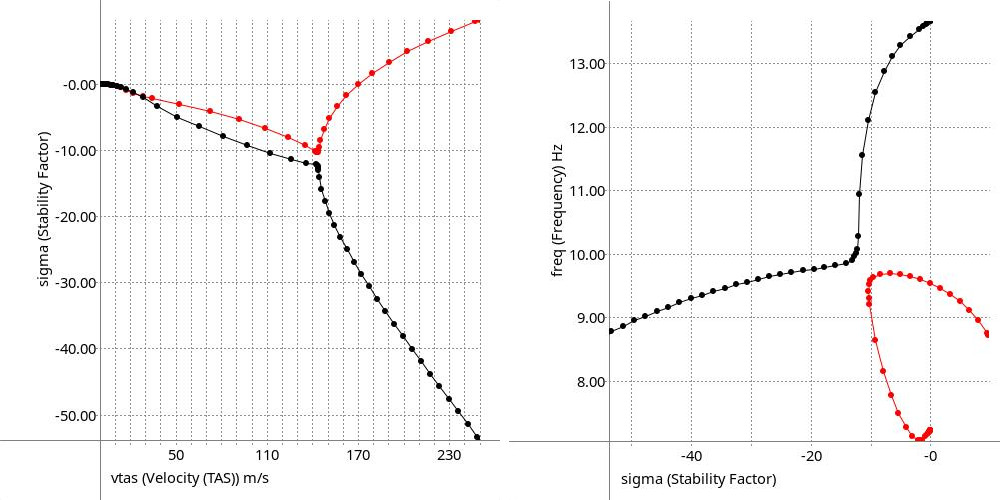
\includegraphics[height=5.5cm,width=12.5cm]{goland-vso.jpg}
	\centering
	\caption{Core flutter results} \label{fig:goland-vso}
\end{figure}

\subsection{Parameter variations}
The effects of certain parameters on the lowest flutter speed are then
studied by varying parameters of interest while holding $\sigma$ zero.
It is well known that 2 parameters that are important for wing flutter are
the position of the center of gravity of the wing and the position of
the aerodynamic center, relative to the elastic axis (\Figref{fig:goland-wing}).

\subsection{Contours}\label{ex:goland-contour}\index{contours}
A parameter, \Code{cg}, is created to give the distance from the elastic
axis to each concentrated mass; giving this name instead of a value
in the \Code{mass} section of \Cmd{fem} results in the output mass matrix
parametrized by a custom evaluation function, the source code for
which is on the current directory.
The second parameter, \Code{ac}, is created to give the distance in
the global x direction of the $3/4$ chord at the root of the doublet-lattice
grid; giving this name instead of a value in the \Code{ac} option of
the \Cmd{dlm} sub-command of the \Cmd{fem} command results in the output
unsteady aerodynamic matrix to have an interpolation parametrization
in (at least) \Code{rf} and \Code{ac}.
\par
In addition to the core flutter results, \Code{ac} and \Code{cg} are used
to demonstrate:
\begin{enumerate}
	\item variation of flutter speed with \Code{ac}
	\item variation of flutter speed with \Code{cg}
	\item continuation-optimization of \Code{vtas} with respect to \Code{ac}
	   and \Code{cg} to get start points for
		contours\index{numerical continuation!optimization}\index{optimization!continuation}
	\item contours of flutter speed with respect to \Code{ac} and \Code{cg}.
\end{enumerate}

\begin{figure}[ht]
		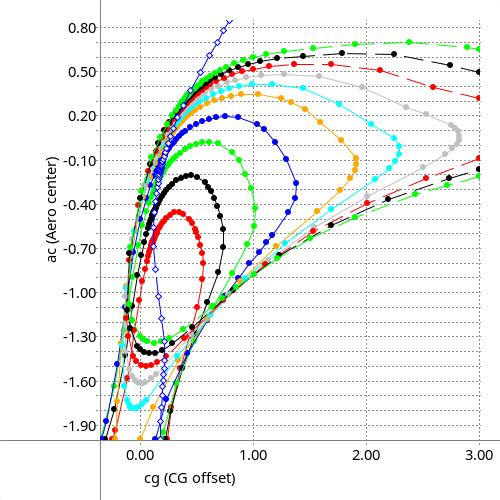
\includegraphics[height=2.5in,width=3.0in]{goland-contour.jpg}
	\centering
	\caption{Velocity contours and optimization}\label{fig:goland-contour}
\end{figure}

Plots of each of these are displayed and may be used to visualize animations
of the mode by right-clicking on the desired points.
Figure \ref{fig:goland-contour} shows the contours together with the optimization
curve used to start the contours.

\subsection{Modal reduction}\label{ex:reduction}
\index{examples!reduction.fp}
Example file reduction.cpp in the examples directory uses the Goland wing to
demonstrate reducing the model size with free vibration modes from 144
degrees-of-freedom to 10. As before, the model is built with the \Cmd{fem}
command, only with a finer grid. The mass, stiffness, and aero matrices
are fed to \Octlab along with a script that does an eigensolution and
triple products with the matrices. Two flutter solutions, one with the
full 144 dof model and the other with the reduced model show very little
difference in the 10 modes tracked.

\section{Formulation comparison}\label{ex:formulation-comp}
As pointed out in \Sectref{sect:formulations},
many different formulations of flutter equations have been proposed
over the past 50 years;
example problem \Code{methods.fp} compares the first 2 modes of the Goland
wing using various formulations of the flutter equation, and the \Fina
solver.
\begin{figure}[ht]
		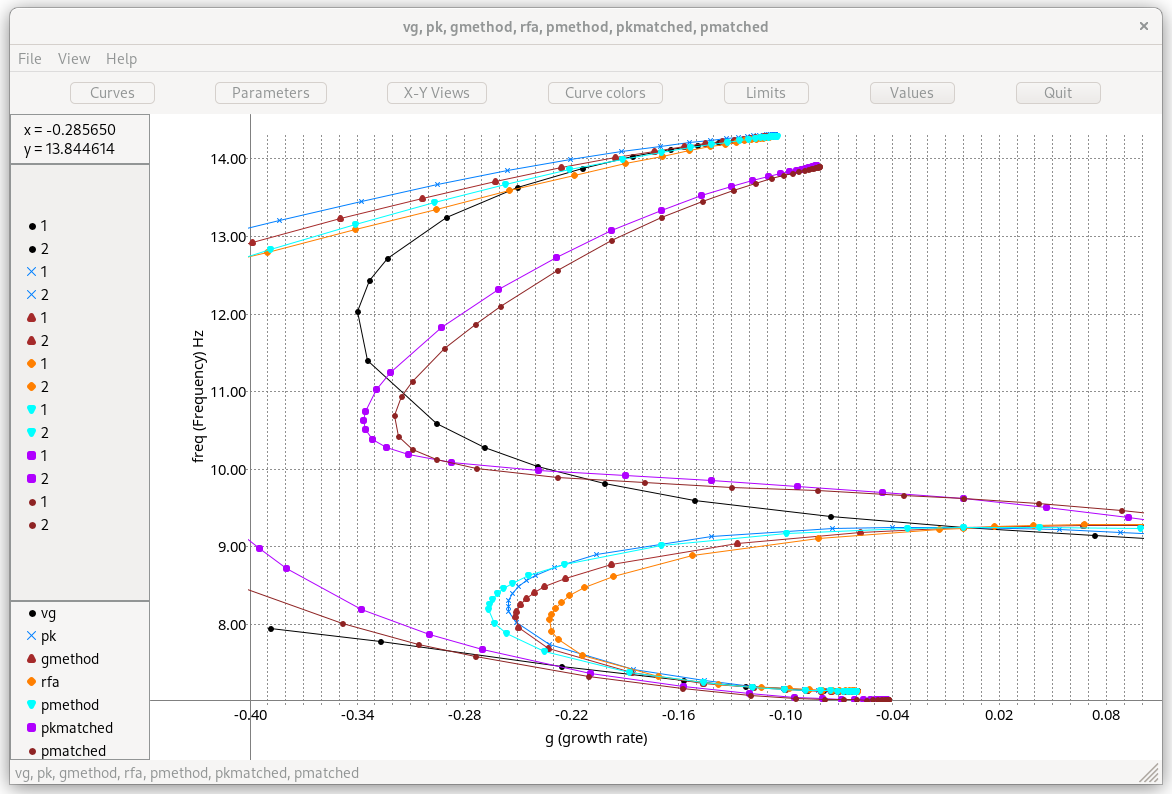
\includegraphics[height=8cm,width=12cm]{methods-g-freq.png}
	\centering
	\caption{2 modes tracked using various formulations: g-freq}
			\label{fig:methodsgf}
\end{figure}
\begin{figure}[ht]
		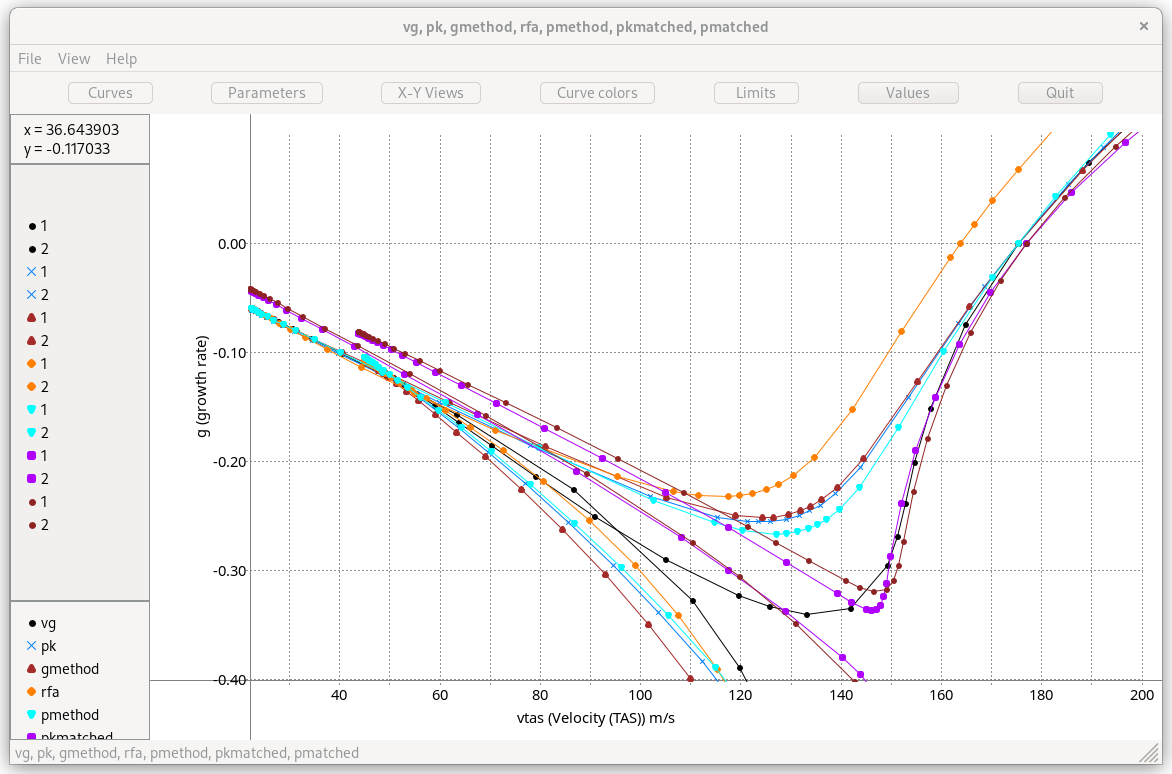
\includegraphics[height=8cm,width=12cm]{methods-v-g.png}
	\centering
	\caption{2 modes tracked using various formulations: vtas-g}
			\label{fig:methodsvg}
\end{figure}
Figures \ref{fig:methodsgf} and \ref{fig:methodsvg}
show this comparison. As expected,
the 2 formulations with matched Mach number give the same flutter speed;
with the exception of the RFA formulation, the other 4 flutter speeds are the
same but different from the matched-Mach curves. RFA, being an approximation,
not an interpolation, gives a slightly different flutter speed.
Besides giving a different flutter speeds, the matched-Mach (and V-g) curves
track differently: mode 1 is stable and mode 2 flutters, opposite from the other 4.

This example problem demonstrates the use of the \Code{process} sub-option
to the \Code{target} option in \Cmd{flut} by specifying a function that
writes some details of the flutter speeds to a local file called \Code{target}.
The source code for this function is at the bottom of \Code{methods.fp}.
\Tableref{table:methods-results} shows the output from this function.
\begin{table}[ht]  % table:methods-results
\centering
\begin{tabular}{|c|c|c|c|} \hline
{\bf id}  &  {\bf mode}      & {\bf vtas m/s}	& {\bf freq Hz}  \\ \hline
vg	&   2 & 175.293 & 58.1161 \\
pk &  1 & 175.293	&	58.1161	\\
gmethod &   1 & 175.29	&	 58.1161 \\
rfa &   1 & 163.81	&	 58.0502 \\
pmethod &   1 & 175.29	&	 58.1161 \\
pkmatched &   2 & 161.63	&	 60.2686 \\
pmatched &   2 & 161.63	&	 60.2686	\\ \hline
\end{tabular}
\caption{\Code{methods.fp} flutter speeds}\label{table:methods-results}\index{parameters!units}
\end{table}

\section{Flight envelope search}\label{ex:envelope-search}
A common task in flutter analysis is searching the flight envelope
for flutter. Example problem \Code{envelope.fp} demonstrates a few
techniques for efficiently searching the envelope.

The model used is the Goland wing with additional concentrated masses
representing fuel (\Figref{fig:goland-fuel}).
Assuming we have a mass matrix parametrized by fuel and possibly payload,
some possible scenarios, all starting with a core (\OSV) analysis at one
or more altitudes:
\begin{itemize}
	\item Any flutter points found are used to start fuel variations
		to see the effect of fuel on flutter speed at that altitude.
	\item Any flutter points found are used to start a
		continuation-optimization process \OPPSV where $p_1$ is fuel and
		$p_2$ is altitude. Anywhere along the optimization
		curve may be used to start a velocity contour. With enough of these
		contours a 3D surface of flutter speed as a function of altitude and
		fuel emerges.\index{contours}
	\item For modes that are stable in the core analyses, choose a few
		velocities and start an altitude-fuel-$\omega$-$\sigma$-$V$\: process,
		optimizing $\sigma$, searching for $\sigma=0$. With several altitudes
		and several stable modes in the core analyses, this type of search
		could involve track many curves but this could be a way to find
		flutter points missed by other techniques.
\end{itemize}

\begin{figure}[ht]
		\includegraphics[height=4cm,width=12cm]{goland-fuel.eps}
	\centering
	\caption{Goland wing with fuel}\label{fig:goland-fuel}
\end{figure}

\section{Substructuring}\label{ex:ss-examples}
Substructuring is also used to reduce the size of models, but more
importantly for flutter is the ability to isolate parts of a structure
to accommodate control systems, nonlinearities, and parameter variations
\Chapref{chap:substructuring}.
Example ss.cpp compares 2 types of dynamic substructuring: Branch Mode
Analysis (BMA) and Component Mode Synthesis (CMS).
Whirl.cpp and whirlnl.cpp demonstrate BMA used for parameter variations
and freeplay nonlinearities. \Figref{fig:ss-compare} is a comparison of the
substructured models and the nodal model.
\begin{figure}[ht]
		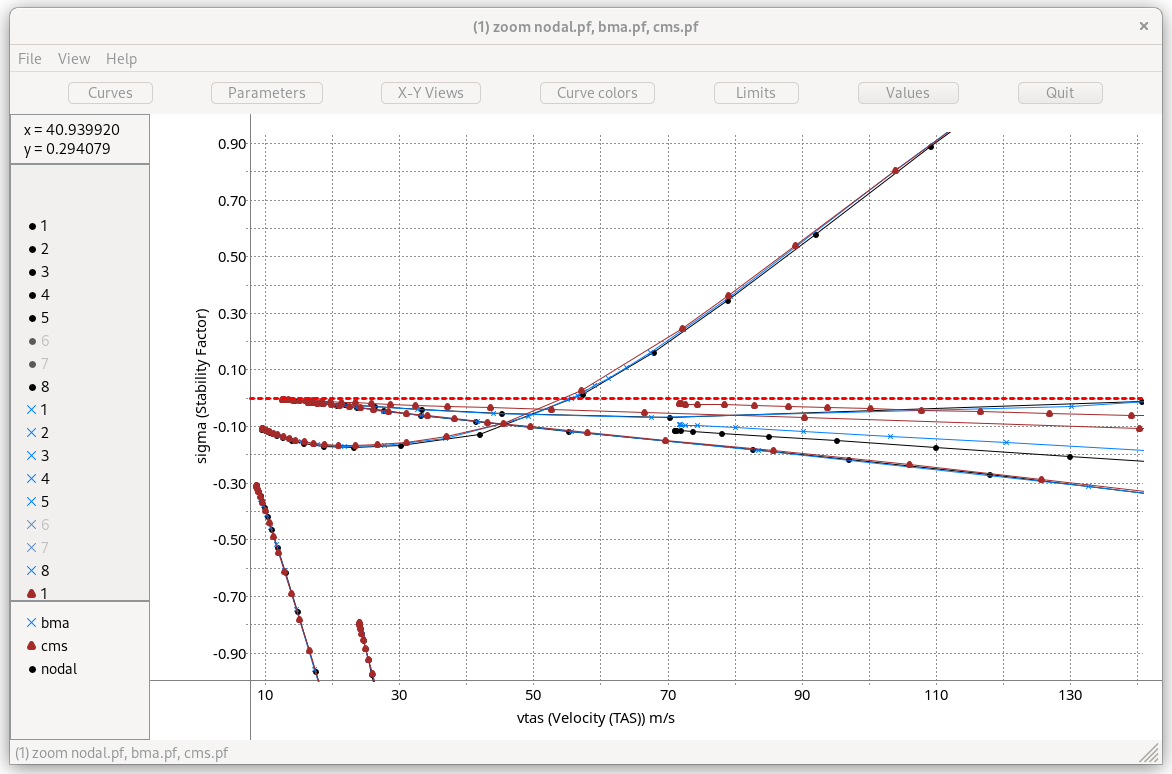
\includegraphics[height=8cm,width=12cm]{ss-compare.png}
	\centering
	\caption{Comparison of BMA, CMS, and nodal-dof models}\label{fig:ss-compare}
\end{figure}

\newpage
\section{Nonlinear flutter}\label{ex:nl1234}
\index{examples!nl[1234].fp}
\Fina offers several ways of creating nonlinear flutter equations,
that is, parametrizing matrices with generalized-coordinate amplitudes.
The first set of problems illustrate these techniques. Next an example
shows how latent LCO can be discovered using the continuation-optimization
technique discussed in \Sectref{sect:optim}.

\subsection{Creating nonlinear equations}
Four small problems demonstrate 4 different ways of including the
same nonlinearities.
These are all based on model HA145b from the MSC/\Nastran Handbook
for Aeroelastic Analysis \cite{rodden2009msc} (which is based on
Example 9-1, p. 565 in \cite{bisplinghoff1955aeroelasticity}),
built with 10 dof.
The first 4 dof have bilinear stiffnesses (\Eqn{eqn:bilinear})
with $\delta = 0.01$ and 3 different ratios: $r_1 = r_2 = 0.5$,
$r_3 = 2$, and $r_4 = 3.5$.

The 4 files implement the bilinear describing functions using 4
different methods, with increasing levels of knowledge of \Cpp
required, but also increasing flexibility:
\begin{description}
\item[nl1.fp] builtin functions are used in equations defined in
\Code{pz}, for example
\begin{lstlisting}
   [1,1] *= bilinear(0.01, 0.5, 1)
\end{lstlisting}
multiplies the [1,1] term by the bilinear describing function with
$\delta=0.01$, $r = 0.5$, and $|\hat{q}_1|$.

\item[nl2.fp] a custom function which does the same multiplication
calling builtin function \Code{df::freeplay}

\item[nl3.fp] uses custom functions to call local custom functions
called \Code{freeplay} and \Code{bilinear}

\item[nl4.fp] a custom function which uses describing functions
created automatically when 3 functions written in \Cpp are included as
a section in the \Fina input file. The 3 functions must have these names and
calling arguments:
	\begin{lstlisting}
vector<double> df_qs(const vector<double>& params)

double df_fq(double y, const vector<double>& params)

Interp* df_interp(const string& iid, const vector<double>& params,
    const vector<double>& qs, const vector<double>& fs)
	\end{lstlisting}
%%	returns a vector with the desired amplitudes
%%	returns the factor which when multiplied by $\Matrix{K}\Vector{y}$ gives the force at the nonlinearity
%% returns a pointer to a new Interp object containing one or more interpolants

\end{description}


\subsection{Latent limit cycles}\label{ex:latent}\index{limit cycle oscillation!latent}
Example problem \Code{latent.fp} shows the discovery of a limit-cycle
that does not go unstable when \Gc\ norm ($\eta$) is zero (latent LCO).
\index{nonlinear flutter}
The model is a simple model of a twin-engine airplane with several nonlinearities:
\begin{itemize}
	\item freeplay on elevator, rudder, and ailerons
	\item bilinear stiffness on nacelle struts
\end{itemize}
The study of limit-cycles involves these \Cmd{flut} processes:
\begin{description}
	\item[\Code{core}] a core flutter analysis: \OSV search for flutter speeds
		with $\eta=0$, i.e. linear flutter points.
	\item[\Code{conopt}] varies $\sigma$, $\omega$ $\eta$ and $V$,
			starting from a stable point on the core analysis and optimizing 
		$\sigma=0$ towards zero.
	\item[\Code{lco}] starting from a $\sigma=0$ point in \Code{conopt}
		traces an LCO curve
\end{description}
\Figref{fig:lco_screen} shows a few latent LCO boundaries discovered using
this set of \Cmd{flut} solutions. The stability of the LCO is indicated by
a change in the color of the curve. A red dot indicates a point that was
clicked on to bring up the animated mode.

\begin{figure}[ht]
		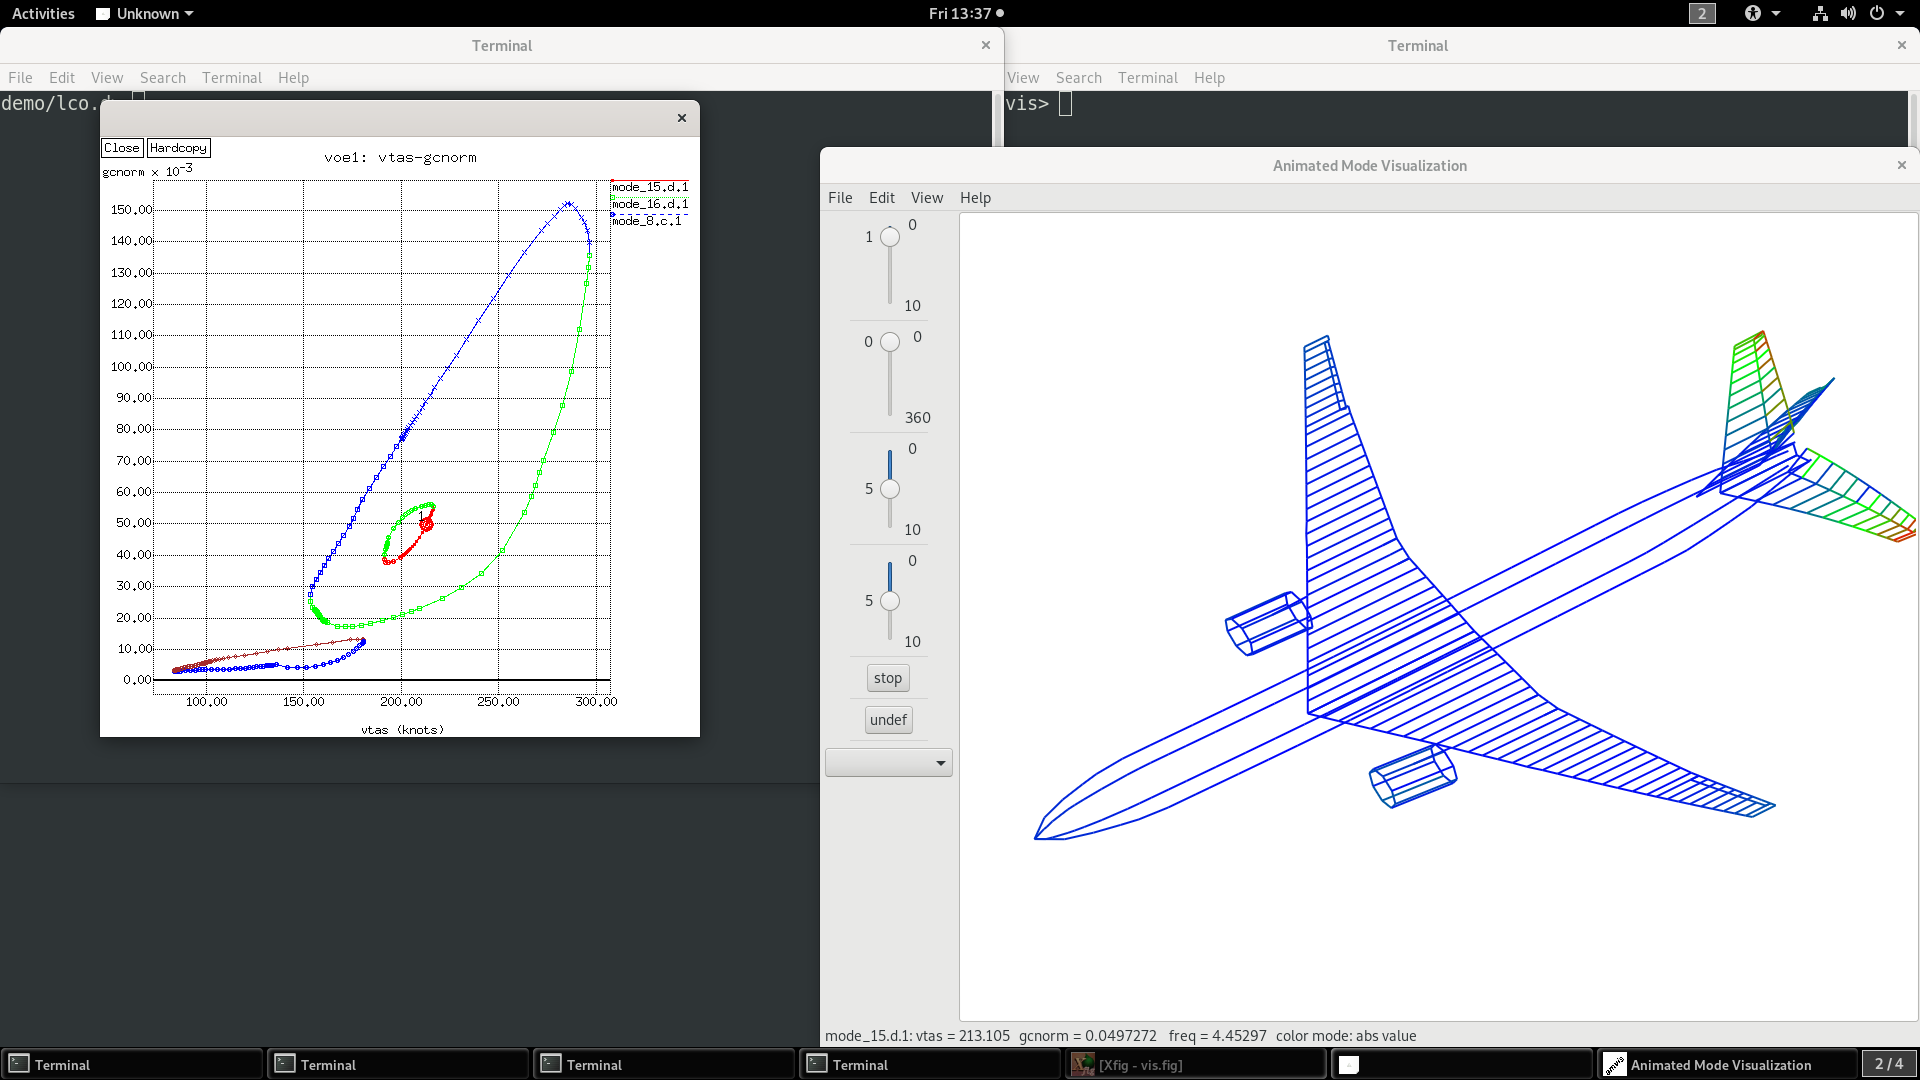
\includegraphics[height=3in,width=4.8in]{lco_screen.png}
	\centering
	\caption{Latent LCO}\label{fig:lco_screen}
\end{figure}

\newpage
\section{Controls Equations}\label{ex:controls}
Two ways of treating control systems in \Fina are shown in files
\Code{lti.fp} and \Code{controls.fp}.

\subsection{Linear-Time-Invariant}
A simple state-space control law (\Sectref{sect:ABCD-file}) is used in
\Code{lti.fp}\index{examples!lti.fp}
to demonstrate the use of \Cmd{octlab} to extract from the modes matrix, \Cmd{lti}
to read a description of the controls equations, and a flutter solution, gain
variation, and phase variation.

\subsection{Custom function}
\index{examples!controls.fp}
Using the same airplane model as in \Sectref{ex:latent}, \Code{controls.fp} uses
a custom function to describe a nonlinear control-system.
The nonlinearities are in the gain, phase, and sensors.
Capabilities demonstrated include
\begin{itemize}
	\item using \Cmd{octlab} to extract 2 rows of the \Code{gctransform}
	    matrix to use in sensor equations
	\item a section of \Cpp code describing the controls equations in
	   the $\Matrix{T}$ matrix.
	\item a \OSV analysis varying reduced-frequency instead of \Code{vtas}
	   so that every solution point produced is within the limits of
		reduced-frequency. The $\Matrix{T}$ matrix is included but with \Code{amp=0}
		it does not affect the solution.
	\item a \OSV analysis including the controls equations with \Code{amp=0}
	   but with a spec, \Code{linearize} which is passed to the
		controls function where the equations are linearized. With these
		linearized controls equations there is a small increase in flutter speed.
	\item a \EOSV analysis to see the effect of increasing the oscillation
	   amplitude on $\sigma$, that is, a search for LCO by driving $\sigma$
		towards zero by a continuation-optimization \index{numerical continuation!optimization}
		with \EOSV.
	\item gain and phase variations to see their influence on linear
	   flutter speed
	\item a gain-phase-frequency-velocity optimization to get start
	   points for velocity contours
	\item gain-phase variations at a few velocities start from the optimization,
	   giving velocity contours.\index{contours}
\end{itemize}

\begin{figure}[ht]
		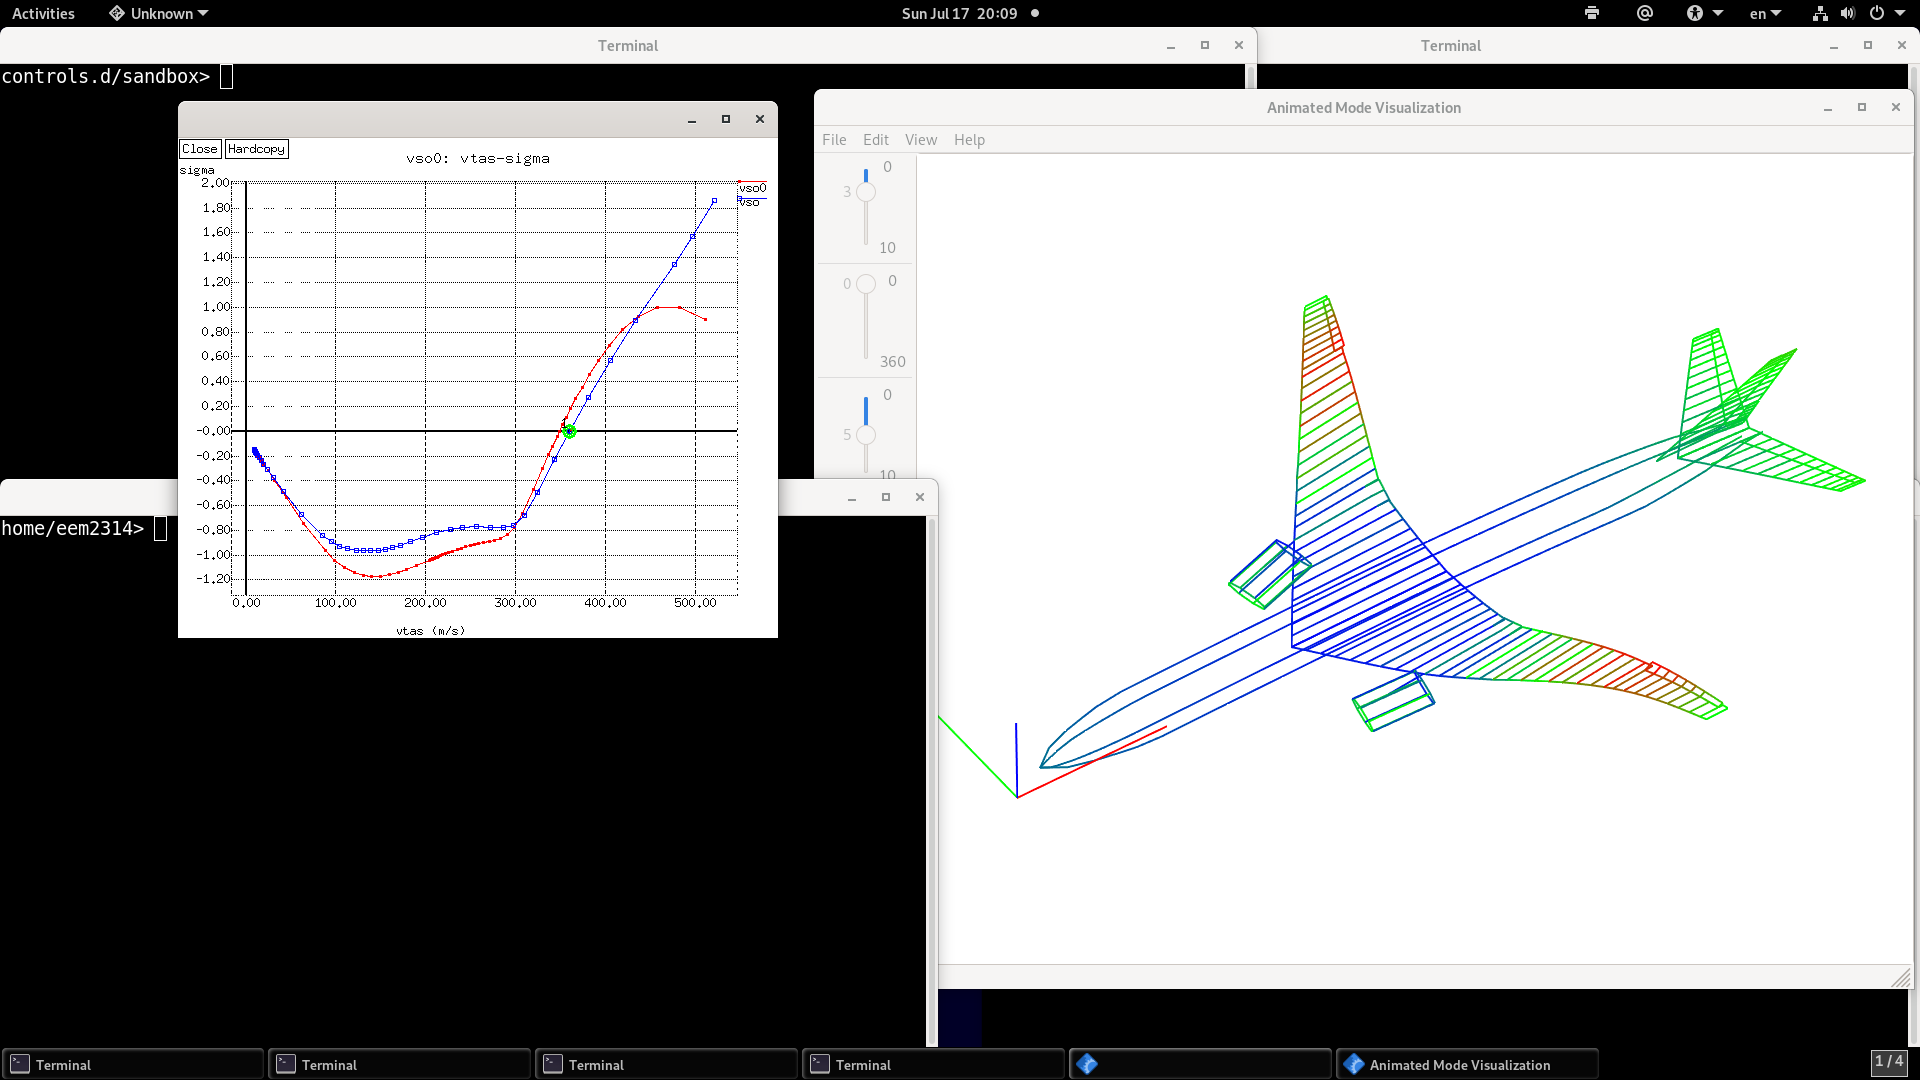
\includegraphics[height=2in,width=3.0in]{controls_vso.png}
	\centering
	\caption{\Code{controls.fp} closed- and open-loop flutter}\label{fig:controls_vso}
\end{figure}

\newpage
\section{Whirl flutter}\label{ex:whirl}\index{whirl flutter}\index{flutter!whirl}
\index{examples!reed.fp}
\index{examples!whirl.fp}
Three example problems illustrate whirl flutter:
\Code{reed.fp} demonstrates whirl flutter on a simple rigid propeller
to validate the \Fina implementation of \cite{reed1961analytical},
\Code{whirl.fp} is the Goland wing with 2
propellers attached, and \Code{whirlnl.fp} is the same but with freeplay
on the propeller mounts. For these a gyro matrix is created with the \Cmd{gyro}
option in \Cmd{fem}, and
unsteady propeller aerodynamics are from \cite{reed1961analytical},
summarized in \Sectref{sect:whirl-aero}, and are implemented
in a custom evaluation function created on the current working directory
(\Code{pgaffcn.cpp}).

The frequency in a whirl flutter analysis is the rate
at which the spinning shaft is precessing about the resting
axis; this precessional\index{precession!frequency} motion can be expressed in revolutions
per minute (rpm) instead of Hertz by changing the definition
of frequency:
\begin{lstlisting}
   parameter{freq(Precessional frequency)[0:10]<radps2rpm>}
\end{lstlisting}
where the builtin constant \Code{radps2rpm} is used here to
change the global definition to
\Code{freq[0:10](Precessional frequency)<9.5493 rpm/(rad/s)>}

Figures \ref{fig:whirl-vso}, \ref{fig:beta}, and \ref{fig:whirl-lbar}
show some results using this aerodynamic model on the simple rigid
propeller in \Code{reed.fp}.
\begin{figure}[hbt!]
	\includegraphics[height=8.0cm,width=8.0cm]{whirl-vso.eps}
%	\includegraphics[height=8.0cm,width=8.0cm]{whirl-vso.pdf}
	\centering
	\caption{V-$\sigma$ at 100 rpm}\label{fig:whirl-vso}
\end{figure}

\begin{figure}[hbt!]
	\includegraphics[height=8.0cm,width=8.0cm]{beta.eps}
\centering
\caption{Variation of flutter speed with blade angle}\label{fig:beta}
\end{figure}

\begin{figure}[hbt!]
	\includegraphics[height=13.0cm,width=8.0cm]{whirl-lbar.eps}
%	\includegraphics[height=13.0cm,width=8.0cm]{whirl-lbar.pdf}
\centering
\caption{Variation of flutter speed and frequency with $l/r$}\label{fig:whirl-lbar}
\end{figure}

\clearpage
\pagebreak

\section{Bifurcation}\label{ex:bifurcation}
\index{bifurcation!example}
Bifurcation, usually associated with nonlinear systems, can occur in
linear flutter analyses, a reminder that even though a flutter analysis
is termed linear because it is independent of generalized coordinate
amplitudes, it is still nonlinear in parameters such as velocity and frequency
\cite{meyer2015continuation}.

Example problem \Code{bif.fp} demonstrates bifurcation in the Goland wing
by changing the moment of inertia about the y axis slightly, causing a
mode to bifurcate, with one branch returning to zero velocity and the
other becoming neutrally stable, as shown in \Figref{fig:bifurcation}.

\begin{figure}[h!]
		\includegraphics[height=7.0cm,width=8.5cm]{bif.eps}
%		\includegraphics[height=7.0cm,width=8.5cm]{bif.pdf}
	\centering
	\caption{Bifurcation in the Goland wing}\label{fig:bifurcation}
\end{figure}

\newpage
% ------------------------------------------------------------------
% Appendices chapter
% ------------------------------------------------------------------
\chapter{Appendices}\label{chap:appendices}

\section{Obtaining the source}\label{sect:obtaining}
Currently the code for \Fina is only available by emailing me
at \Code{flapsconsulting@gmail.com}. I'm sorry for the inconvenience.

\section{Installation}\label{sect:installation}
To install \Fina from a distribution tar file, e.g.
fina-1.6.1.tar.gz

Assuming a Linux operating system
\footnote{there are dozens of Linux distributions; the important thing here is
the package manager used. The 3 main package managers used in Linux
distros are apt, dnf (yum), and pacman. The PACKAGE script used here
lists the packages for apt and dnf; it should be easy to modify them
to work with pacman, which is used in distros based on Arch Linux.
Likewise for the less-used package managers like portage, zypper, and xbps.}
and starting in the directory containing the tar file:
\begin{lstlisting}
>  tar zxf fina-XXX.tar.gz
\end{lstlisting}
will create a directory \Code{fina-XXX}, the \Fina root directory,
populated with the source files necessary to build \Fina.

If this is the first time installing \Fina it may be necessary to
install certain packages; the PACKAGES file in the \Fina root directory
can be run as a script like this:
\begin{lstlisting}
> yes | sudo PACKAGES
\end{lstlisting}
note that it is usually necessary to run it as superuser with sudo.
PACKAGES will try to determine if this Linux uses apt or rpm for
package management.

Once you have the necessary packages installed all you should have
to do is
\begin{lstlisting}
>  cd fina-XXX
>  ./configure --prefix=directory-where-to-install
>  make install
\end{lstlisting}

If this is successful you can run some tests:
\begin{lstlisting}
>  cd examples
>  run all
\end{lstlisting}

If the build is not successful it may be because some packages
were not installed, or it may be necessary to adjust environment
variables.

Or maybe it is time to text or email
\begin{lstlisting}
Ed Meyer
206-453-8778
flapsconsulting@gmail.com
\end{lstlisting}

% ------------------------------------------------------------------
\newpage
\section{Atmospheric properties}\label{sect:atmos}
\Tableref{table:atmos} list properties of the standard atmosphere
from \cite{united1976us}.

\begin{table}[h]  % table:atmos
\begin{tabular}{|c|c|c|c|c|c|c|c|c|c|} \hline
{\bf Altitude } & {\bf Temperature}  & {\bf Pressure} & {\bf Density} & {\bf Sonic Velocity} \\
$Km$            & $\deg K$           & $Pa$ ($N/m^2$)        & $kg/m^3$      & $m/s$ \\ \hline
  -2 & 301.2 & 127800 & 1.478 & 347.9 \\ \hline
   0 & 288.150 & 101325 & 1.225 & 340.3 \\ \hline
   2 & 275.2 & 79500 & 1.007 & 332.5 \\ \hline
   4 & 262.2 & 61660 & 0.8193 & 324.6 \\ \hline
   6 & 249.2 & 47220 & 0.6601 & 316.5 \\ \hline
   8 & 236.2 & 35650 & 0.5258 & 308.1 \\ \hline
  10 & 223.3 & 26500 & 0.4.135 & 299.5 \\ \hline
  12 & 216.6 & 19400 & 0.3119 & 295.1 \\ \hline
  14 & 216.6 & 14170 & 0.2279 & 295.1 \\ \hline
  16 & 216.6 & 10350 & 0.1665 & 295.1 \\ \hline
  18 & 216.6 & 7565 & 0.1216 & 295.1 \\ \hline
  20 & 216.6 & 5529 & 0.08891 & 295.1 \\ \hline
  22 & 218.6 & 4048 & 0.06451 & 296.4 \\ \hline
  24 & 220.6 & 2972 & 0.04694 & 297.7 \\ \hline
  26 & 222.5 & 2188 & 0.03426 & 299.1 \\ \hline
  28 & 224.5 & 1616 & 0.02508 & 300.4 \\ \hline
  30 & 226.5 & 1197 & 0.01841 & 301.7 \\ \hline
  40 & 250.3 & 287.1 & 0.003996 & 317.2 \\ \hline
  50 & 270.6 & 79.78 & 0.001027 & 329.8 \\ \hline
  60 & 247.0 & 21.96 & 0.0003097 & 315.1 \\ \hline
  70 & 219.6 & 5.221 & 8.283(-5) & 297.1 \\ \hline
  80 & 198.6 & 1.052 & 1.846(-5) & 282.5 \\ \hline
\end{tabular}
\caption{Atmospheric properties} \label{table:atmos}
\index{atmospheric properties}
\index{altitude}
\index{density}
\index{temperature}
\index{pressure!static}
\index{static pressure}
\index{sonic velocity}
\end{table}

\newpage
\section{Rational-Function Approximation (RFA)}\label{chap:RFA}
\index{s-plane approximation|see{rational-function approximation}}
\index{RFA|see{rational-function approximation}}
\index{rational-function approximation|textbf}
Unsteady aerodynamics used for flutter calculations are typically
functions of reduced frequency ($\bar{\omega}$). It is sometimes desirable
to improve the accuracy of growing or decaying amplitude ($\sigma \ne 0)$)
flutter solutions by extending the domain to complex reduced frequency
($\bar{s} = \frac{s}{V} = \bar{\sigma} + i\bar{\omega})$.
Two common ways to do this are with 2-way interpolation and
with a rational-function approximation. Differences between
these 2 approaches include
\begin{itemize}
	\item an interpolation matches the original set of matrices
		exactly; an approximation in general matches approximately.
			\index{aerodynamics!interpolation vs approximation}
	\item a ($\bar{\sigma}, \bar{\omega}$) interpolation requires
		an unsteady aerodynamics code capable of producing matrices
		at non-zero values of $\bar{\sigma}$ \cite{edwards2008flutter}
	\item an interpolation must have first-derivative continuity
		to satisfy the requirements of the continuation method; the
		approximation presented here meets that requirement.
	\item approximations require a measure of the error in the
		fit; least-squares is a very common measure.
\end{itemize}

The most commonly used RFA is due to Roger \cite{roger1977airplane}.
It comprises a quadratic polynomial in $\bar{s}$ and a set of rational
polynomials in $\bar{s}$ and real constants $\beta_i$, known as
lag roots. Details regarding the $\beta_i$ and their physical
significance can be found in \cite{demasi2024introduction}, along
with critera for selecting the number and values of them.

Assuming a set of $m$ unsteady aerodynamic matrices, functions of reduced frequency $\bar{\omega}$:
\begin{equation}
\Matrix{Q}_k = \Matrix{Q}(\bar{\omega}_k) = \left[Q_{ij,k}\right]
			\hspace{5mm} (k = 1, m) \; \; \in \mathbb{C}^{n \times n},
\end{equation}
Roger's method approximates them with a function of $\bar{s}$ 
and a set of $\ell$ positive, real \emph{lag roots} $\beta_i, i=1,\ell$:
\begin{equation}
  \Matrix{Q}(\bar{s}) \approx \Matrix{R}_0 + \bar{s}\Matrix{R}_1 + \bar{s}^2 \Matrix{R}_2 +  \sum_{l=1}^{\ell} \frac{\bar{s}}{\bar{s} + \beta_l} \Matrix{R}_{l+2}
\end{equation}
where the $\ell + 3$ matrices
$\Matrix{R}_0, \Matrix{R}_1, \ldots, \Matrix{R}_{\ell+2}$ are real.
Each element
\begin{displaymath}
R_{ij,0}, R_{ij,1}, \ldots, R_{ij,\ell+2}
\end{displaymath}
is determined by $2m$ equations, comprising the real and imaginary parts
of the $m$ $\Matrix{Q}$ matrices:
\begin{align}
	\Re(R_{ij,0} + \bar{s}_k R_{ij,1}
  		+ \bar{s}_k^2 R_{ij,2} +  \sum_{l=1}^{\ell} \frac{\bar{s}_k}{\bar{s}_k +
			\beta_l} R_{ij,l+2}) &= \Re(A_{ij,k}) \nonumber	\\
	\Im(R_{ij,0} + \bar{s}_k R_{ij,1}
  		+ \bar{s}_k^2 R_{ij,2} +  \sum_{l=1}^{\ell} \frac{\bar{s}_k}{\bar{s}_k +
			\beta_l} R_{ij,l+2}) &= \Im(A_{ij,k})	\nonumber
\end{align}
from which we can determine the $(i,j)$ elements of the $\Matrix{R}$ matrices:
$(\ell+3)$ unknowns. Provided $2m > \ell+3$ these equations are overdetermined
and can be solved by least-squares:
\begin{equation}
\Matrix{S}\Vector{x} = \Vector{b}
\end{equation}
where
\begin{displaymath}
\Matrix{S} = \left[
\begin{array}{cccccc}
1 & \Re(\bar{s}_1) & \Re(\bar{s}_1^2) & \Re(\frac{\bar{s}_1}{\bar{s}_1 + \beta_1}) & \ldots & \Re(\frac{\bar{s}_1}{\bar{s}_1 + \beta_{\ell}}) \\
0 & \Im(\bar{s}_1) & \Im(\bar{s}_1^2) & \Im(\frac{\bar{s}_1}{\bar{s}_1 + \beta_1}) & \ldots & \Im(\frac{\bar{s}_1}{\bar{s}_1 + \beta_{\ell}}) \\
1 & \Re(\bar{s}_2) & \Re(\bar{s}_2^2) & \Re(\frac{\bar{s}_2}{\bar{s}_2 + \beta_1}) & \ldots & \Re(\frac{\bar{s}_2}{\bar{s}_2 + \beta_{\ell}}) \\
0 & \Im(\bar{s}_2) & \Im(\bar{s}_2^2) & \Im(\frac{\bar{s}_2}{\bar{s}_2 + \beta_1}) & \ldots & \Im(\frac{\bar{s}_2}{\bar{s}_2 + \beta_{\ell}}) \\
  &          &            &                                & \ddots &                           \\
1 & \Re(\bar{s}_m) & \Re(\bar{s}_m^2) & \Re(\frac{\bar{s}_m}{\bar{s}_m + \beta_1}) & \ldots & \Re(\frac{\bar{s}_m}{\bar{s}_m + \beta_{\ell}}) \\
0 & \Im(\bar{s}_m) & \Im(\bar{s}_m^2) & \Im(\frac{\bar{s}_m}{\bar{s}_m + \beta_1}) & \ldots & \Im(\frac{\bar{s}_m}{\bar{s}_m + \beta_{\ell}}) \\
\end{array}
\right]	\hspace{3mm} \in \mathbb{R}^{2m\times \ell+3}
\end{displaymath}

\begin{displaymath}
\Matrix{x} = \left\{
\begin{array}{c}
R_{ij,0} \\
R_{ij,1}  \\
\ddots  \\
R_{ij,\ell+2}
\end{array}
\right\}		\hspace{3mm} \in \mathbb{R}^{\ell+3}
\end{displaymath}

\begin{displaymath}
 \Matrix{b} =
\left\{
\begin{array}{c}
\Re(Q_{ij,1}) \\
\Im(Q_{ij,1}) \\
\Re(Q_{ij,2}) \\
\Im(Q_{ij,2}) \\
\ddots \\
\Re(Q_{ij,m}) \\
\Im(Q_{ij,m})
\end{array}
\right\}		\hspace{3mm} \in \mathbb{R}^{2m}
\end{displaymath}
The coefficient matrix $\Matrix{S}$ is the same for all elements of the
$\Matrix{R}$ matrices so all $n^2$ elements can be computed simultaneously
with, for example Lapack routine \Code{DGELSS} \cite{anderson1999lapack}.

\newpage
\section{Concurrency}\label{sect:concurrency}
Concurrency in a computer program refers to the ability to do 2 or
more things simultaneously. Also known as \Newterm{parallel execution},
concurrency can speed up a program dramatically if it is run on a platform
which allows for multiple \Newterm{threads} of execution on multiple cores
\cite{williams2009c++}.
Each thread can share data with other threads, which can lead to errors that
are extremely hard to find if a thread modifies data which is then accessed by
other threads, since the timing of the modifications and accesses can lead
to different results. Concurrent program must be done carefully, always mindful
of this and other hazards
\cite{williams2009c++}.
\par
Solving the flutter equation with numerical continuation allows for
concurrent execution because each mode that is tracked is completely
independent of other modes, a situation that has been called
``embarrassingly parallelizable''.
\par
Two places in \Cmd{flut} are easily parallelized:\index{numerical continuation!parallelized}
the homotopy process for
finding start points, and the actual tracking of each mode. When run on a
computer with, e.g. an AMD Ryzen 7 with 8 cores and 16 threads, 16 modes
at a time are tracked, results are stored and fetched when all 16 threads have
finished for post-processing.
The only data that must be shared between threads are the matrices that
make up the problem. These are not modified by threads, only copied to form
the dynamic matrix.
\par
\Cpp supports concurrent program in the standard \Cpp library; very little extra
coding is necessary, and no extra libraries are needed.

% ------------------------------------------------------------------
\section{Extended convergence criteria}\label{sect:ecc}
\index{convergence!extended}
Continuation methods sometimes are given problems where the function
$\Vector{f(x)}$
has elements that differ by many orders of magnitude. The usual criterium
for determining convergence of an iterative scheme like Newton's method,
\begin{equation}
\label{eqn:tradcc}
\| \Vector{f} \| < \epsilon_{a} \hspace{0.2in} \text{and} \hspace{0.2in} \| \Vector{h} \| < \epsilon_{a} + \epsilon_{r}\| \Vector{x} \|
\end{equation}
does not account for this variation, and may result in convergence being
declared prematurely. Here an attempt is made to account for these variations.

Given an $\Vector{x}$ that is near a solution, assume it is contained
within a small interval of the exact
solution $(\Vector{\tilde{x}})$
\begin{align}
\Vector{x} &\in \tilde{\Vector{x}} \pm \Vector{r} \nonumber \\
|x_i - \tilde{x}_i| &\le r_i = \epsilon |x_i|
\end{align}
where $\epsilon$ is a multiple of the machine roundoff error.
The corresponding interval in $\Vector{f}$ is approximately
\begin{equation}
\Vector{\tilde{f}} \approx \Vector{f(\tilde{x})} \pm \Vector{f}' \Vector{r}
	= \pm \Matrix{J}\Vector{r}
\end{equation}
so the extended convergence criteria is
\begin{equation}
f_i \le \epsilon \sum_{j=1}^{n} |J_{ij} x_i| = \epsilon_i
\end{equation}
This same method can be used to compute $\epsilon_a$ in \Eqn{eqn:tradcc} as
\begin{equation}
\epsilon_a = \sqrt{\sum_{i=1}^{m} \epsilon_i} = \|\{\epsilon_i\}\|_2
\end{equation}
provided the ratio of the smallest to largest $\epsilon_i$ is not too small.


\section{File Formats}
This section documents a few of the file formats used in \Fina; they
are ASCII file so you may edit, modify or create them.

\subsection{ASCII plot file (.apf) format}\label{sect:apf-file}
This section describes the format of ASCII plot files produced by
\Cmd{flut} to allow the user to create his own files or modify ones
from \Cmd{flut}.
Because they are ASCII files
you can edit them and move them across platforms.
\index{apf plot files!file format}

Comment lines start with a number sign (\#) and
are ignored.
The format is free-field: numbers do not need to
appear in specific columns of a line.

The file consists of blocks of data terminated by a line with
only the characters \Code{*EOF} starting in column 1. Each block
contains data for \Code{npar} parameters at \Code{npt} points.
\begin{description}
	\item[1 line] (optional) a line starting with a dollar sign and
		the rest of the line a title for the plot 
	\item[parameter descriptions] (optional) lines beginning with '+' and the parameter number
			followed by a description of the parameter for the plot axes
	\item[1 line] (required) a single word to identify the following
			data, e.g. in the plot legend
	\item[1 line] (required) \Code{npar} words separated by spaces naming each
			parameter
	\item[\Code{npt} lines] (\Code{npar} floating point numbers per line)
			each line contains the parameter values at one point
	\item[1 line] (required) \Code{*EOF}
\end{description}

\subsubsection{Example} A simple example with 2 blocks of data and
3 parameters in each.
\begin{lstlisting}
$ mode_1
+1 Dynamic Pressure
+2 Frequency
+3 Stability Factor
mode_1
 dpress freq sigma
 5.498228387430155 1.304760601942483 -0.01365279838940575
 5.503767664540073 1.304765132272082 -0.01365876439469717
*EOF
$ mode_2
+1 Dynamic Pressure
+2 Frequency
+3 Stability Factor
mode_2
 dpress freq sigma
 6.4e+2 2.3 -2.01e-03
 6.5e+2 2.4 -2.03e-03
*EOF
\end{lstlisting}

\subsection{Universal File Formats}\label{sect:universal-file}
\index{universal-file!format}
Universal files are used to import data used to visualize animated
flutter modes.
The ASCII file formats described here are considered obsolete by the
developers, the University of Cincinnati Structural Dynamics Research Lab,
but they are still documented at \cite{UniversalFile}. Documentation for
the formats used in \Fina (Datasets 15, 55, and 82) are included here
for convenience. Only the relevant items are shown. Datasets are enclosed
by lines containing only -1 beginning in column 5.
\par
\begin{verbatim}

Universal Dataset Number 15
Name:   Nodes
Status: Obsolete
Owner:  Simulation
Revision Date: 30-Aug-1987
Additional Comments: This dataset is written by I-DEAS Test.
-----------------------------------------------------------------------

             Record 1: FORMAT(4I10,1P3E13.5)
                       Field 1 -    node label
                       Field 2 -    definition coordinate system number
                       Field 3 -    displacement coordinate system number
                       Field 4 -    color
                       Field 5-7 -  3 - Dimensional coordinates of node
                                    in the definition system

             NOTE:  Repeat record for each node

------------------------------------------------------------------------------

Universal Dataset Number 55
Name:   Data at Nodes
Status: Obsolete
Owner:  Simulation
Revision Date: 07-Mar-1997
Additional Comments: This dataset is written and read by I-DEAS Test.
-----------------------------------------------------------------------

          RECORDS 1-5:      Format (40A2)
               FIELD 1:          ID Line

          RECORD 6:      Format (6I10)

          Data Definition Parameters

               FIELD 1: Model Type
                           1:   Structural

               FIELD 2:  Analysis Type
                           3:   Complex eigenvalue first order

               FIELD 3:  Data Characteristic
                           2:   3 DOF Global Translation
                                Vector

               FIELD 4: Specific Data Type
                           8:   Displacement

               FIELD 5:  Data Type
                           2:   Real
                           5:   Complex

               FIELD 6:  Number Of Data Values Per Node (NDV)


          Records 7 And 8 Are Analysis Type Specific

          General Form

          RECORD 7:      Format (8I10)

               FIELD 1:          Number Of Integer Data Values
                           1 < Or = Nint < Or = 10
               FIELD 2:          Number Of Real Data Values
                           1 < Or = Nrval < Or = 12
               FIELDS 3-N:       Type Specific Integer Parameters


          RECORD 8:      Format (6E13.5)
               FIELDS 1-N:       Type Specific Real Parameters


          For Analysis Type = 3, Complex Eigenvalue

          RECORD 7:
               FIELD 1:    2
               FIELD 2:    6
               FIELD 3:    Load Case Number
               FIELD 4:    Mode Number

          RECORD 8:

               FIELD 1:    Real Part Eigenvalue
               FIELD 2:    Imaginary Part Eigenvalue
               FIELD 3:    Real Part Of Modal A
               FIELD 4:    Imaginary Part Of Modal A
               FIELD 5:    Real Part Of Modal B
               FIELD 6:    Imaginary Part Of Modal B


          RECORD 9:      Format (I10)

               FIELD 1:          Node Number

          RECORD 10:     Format (6E13.5)
               FIELDS 1-N:       Data At This Node (NDV Real Or
                         Complex Values)

          Records 9 And 10 Are Repeated For Each Node.


          Notes:
          1        Id Lines May Not Be Blank.  If No Information Is
                      Required, The Word "None" Must Appear  Columns 1-4.

          2        For Complex Data There Will Be 2*Ndv Data Items At Each
                      Node. The Order Is Real Part For Value 1,  Imaginary
                      Part For Value 1, Etc.
          3        The Order Of Values For Various Data  Characteristics
                      Is:
                          3 DOF Global Vector:
                                  X, Y, Z

          4        Id Line 1 Always Appears On Plots In Output Display.
          5        If Specific Data Type Is "Unknown," ID Line 2 Is
                      Displayed As Data Type In Output Display.

          7        Data Characteristic Values Imply The Following Values
                      Of Ndv:
                                      3 DOF Global Vector: 3

          9        Any Record With All 0.0 Data Entries Need Not (But
                      May) Appear.

          10       A Direct Result Of 9 Is That If No Records 9 And 10
                      Appear, All Data For The Data Set Is 0.0.

          12       Dataloaders Use The Following ID Line Convention:

                              1.   (80A1) Model
                                  Identification
                              2.   (80A1) Run
                                  Identification
                              3.   (80A1) Run
                                  Date/Time
                              4.   (80A1) Load Case
                                  Name

          13       No Maximum Value For Ndv .

----------------------------------------------------------------------

Universal Dataset Number 82
Name:   Tracelines
Status: Obsolete
Owner:  Simulation
Revision Date: 27-Aug-1987
Additional Comments:  This dataset is written by I-DEAS Test.
-----------------------------------------------------------------------

             Record 1: FORMAT(3I10)
                       Field 1 -    trace line number
                       Field 2 -    number of nodes defining trace line
                                    (maximum of 250)
                       Field 3 -    color

             Record 2: FORMAT(80A1)
                       Field 1 -    Identification line

             Record 3: FORMAT(8I10)
                       Field 1 -    nodes defining trace line
                               =    > 0 draw line to node
                               =    0 move to node (a move to the first
                                    node is implied)
             Notes: 1) MODAL-PLUS node numbers must not exceed 8000.
                    2) Identification line may not be blank.
                    3) Systan only uses the first 60 characters of the
                       identification text.
                    4) MODAL-PLUS does not support trace lines longer than
                       125 nodes.
                    5) Supertab only uses the first 40 characters of the
                       identification line for a name.
                    6) Repeat Datasets for each Trace_Line

\end{verbatim}

\subsection{LTI File Format}\label{sect:ABCD-file}
This section describes the format of ASCII file produced by SIMULINK
to represent an LTI control system.
Because they are ASCII files
you can edit them and move them across platforms.
\index{LTI control system!file format}

Comment lines start with a number sign (\#) and
are ignored.
The format is free-field: numbers do not need to
appear in specific columns of a line.
\par
In the following description of the file format a
number of variables are used:
\begin{description}
	\item[$ns$] the number of rows and columns in the A matrix,
                the number of rows in B and the number of columns in C
	\item[$ni$] the number of inputs; the number of columns in B and D.
	\item[$no$] the number of outputs; the number of rows in C and D.
	\item[$nb$] the number of breakpoints in the A matrix interpolant.
	\item[$nix$] the number of elements of A which are interpolated
	\item[$nin$] the number of elements of A which are constant
	\item[$ntd$] the number of internal time delays
	\item[$ntdi$] the number of elements of A effected by the
						$i^{th}$ internal time delay
\end{description}
\par
The file consists of blocks of data:
\begin{description}
	\item[1 line] 6 integers: $ns\; ni\; no\; nb\; nix\; nin$
	\item[1 line] (string) Name of the parameter used to interpolate the
		A matrix (e.g. alt or vcas)
	\item[$nb$ lines] (1 float per line) values of the variable used
                to interpolate A at the breakpoints
	\item[$nix$ lines] (2 integers per line) row and column indices of the elements
                of A which are interpolated
	\item[$nin$ lines] (2 integers per line) row and column indices of the elements
                of A which are constant (seems redundant).
	\item[$ni$ lines] (1 float per line) input time delays
	\item[$no$ lines] (1 float per line) output time delays
	\item[$ni$ lines] (1 float per line) exponents of s in the S matrix
                (see \Eqn{eqn:abcd-ui}).
   \item[$ns*ns$ lines] (1 float per line) elements of the A matrix by rows
	\item[$ns*ni$ lines] (1 float per line) elements of the (ns,ni) B matrix by rows
   \item[$no*ns$ lines] (1 float per line) elements of the (no,ns) C matrix by rows
	\item[$no*ni$ lines] (1 float per line) elements of the (no,ni) D matrix by rows
	\item[$(nb-1)*4*nix$ lines] (1 float per line) coefficients for interpolating
                the A matrix: a (nb-1, 4, nix) array stored as
			\nopagebreak
			{\scriptsize \ttfamily
			\begin{verbatim}
			(((coef(i,j,k), j=1,4), i=1,nb-1), k=1,nix)
			\end{verbatim}
			}
			\nopagebreak
	\item[1 line] (1 integer) number of internal time delays ($ntd$). Following
				this line will be ntd repetitions of the next 2 blocks
	\begin{description}
		\item[1 line] (1 integer) number of elements of A affected by this
				time delay ($ntdi$)
		\item[$ntdi$ lines] (2 integers per line) row and column indices of the elements
                of A which are affected by this time delay.
	\end{description}
	\item[$ntd$ lines] (1 float per line) time delays
\end{description}

% ------------------------------------------------------------------

\newpage

\printbibliography[heading=bibintoc]

\newpage
\phantomsection
\printindex

\end{document}
